\documentclass[a4paper,10pt, twocolumn, twoside, titlepage]{article}
\usepackage{fullpage}
%\usepackage[scaled=0.85]{helvet}
\renewcommand{\familydefault}{\sfdefault}
\usepackage{ucs}
\usepackage[utf8x]{inputenc}
\usepackage[brazil]{babel}
\usepackage[T1]{fontenc}
\usepackage{lmodern}
\usepackage[pdftex]{graphicx}
\usepackage{url,color,float}
\usepackage{multirow}
\usepackage{hyperref}
\hypersetup{
    colorlinks=false,
    pdfborder=0 0 0
}
\usepackage{multicol}
\usepackage{fancyhdr}
\usepackage{wallpaper}

%%%%% Headers and Footers
\pagestyle{fancy}
\fancyhf{}
\fancyhead[LE, RO]{Manual do Bixo}
\fancyhead[RE, LO]{\leftmark}
\fancyfoot[EL, OR]{\thepage}
\fancyfoot[RE, LO]{CACo - Centro Acadêmico da Computação}
\renewcommand{\headrulewidth}{0.2pt}
\renewcommand{\footrulewidth}{0.2pt}
\renewcommand{\headsep}{15pt}
\renewcommand{\footskip}{30pt}
\renewcommand{\textheight}{642pt}
\renewcommand{\voffset}{0pt}


\begin{document}

%%%% Capa
\thispagestyle{empty}
\ThisTileWallPaper{\paperwidth}{\paperheight}{img/capa.png}

\pagebreak{4}

%%%% Final da capa

\onecolumn

\begin{figure}
    \centering
    
\includegraphics[scale=0.50,keepaspectratio=true]{img/caco-logo-grande.png}
\end{figure}

\paragraph{}
Bem vindo!

\paragraph{}
Este é o Manual do Bixo do CACo, o Centro Acadêmico da Computação.
Ele foi elaborado por seus veteranos e inclui diversas dicas para auxiliar a sua
sobrevivência neste primeiro ano na Unicamp =).
Você provavelmente recebeu a versão impressa nas primeiras semanas de aula(se
não, passe na salinha do CACo/AAACEC para pegar).

\paragraph{}
Aproveite!

\vfill % o vfill é pra jogar o texto na licença pro final da página

\begin{figure}[H]
    \centering
    
\includegraphics[scale=0.70,keepaspectratio=true]{img/cc_logo.png}
\end{figure}

\paragraph{}
Este trabalho está licençiado sob a Licença Attribution-ShareAlike 2.5 Brazil
da Creative Commons. Para ver uma cópia desta licença,
visite \url{http://creativecommons.org/licenses/by-sa/2.5/br/} ou envie uma
carta para Creative Commons, 444 Castro Street, Suite 900, Mountain View,
California, 94041, USA.

\begin{figure}[H]
    \centering
    
\includegraphics[scale=0.50,keepaspectratio=true]{img/by-sa.png}
\end{figure}

\begin{center}
    Copyright \copyright  2011 Centro Acadêmico da Computação
\end{center}

\clearpage

\tableofcontents
\clearpage
\onecolumn

%%%%% Bem vindo
% Este arquivo tex vai ser incluído no arquivo tex principal, não pe preciso
% declarar nenhum cabeçalho

\section{Bem-vindo a um mundo novo!}

Olá, bixo! Seja bem-vindo! Agora que você está na faculdade, pode ser que aprenda que aquele estereótipo de nerd
da escola não lhe garante boas notas, e que o lugar onde você mais vai aprender não
é a sala de aula. É verdade, calouro, a faculdade é diferente, e quase tudo
dependerá de você, desde quais matérias quer cursar até quando vai estudar para
as provas. Portanto, leia isto com atenção.

Os professores, salvo raras exceções, dificilmente saberão seu nome ou quem é você; provavelmente, eles só verão
no final do semestre se o RA 127654  passou ou não passou. Mas não se sinta
desamparado, afinal, você também vai logo esquecer a matéria deles! O quanto você
estuda não é diretamente proporcional à sua nota, portanto aprenda a estudar
melhor. Atividades em grupo, resolução de exercícios e monitorias são boas pedidas.

Mas a Universidade não se resume a estudo. Você vai conhecer muita gente nova e
descobrir que a vida acadêmica vai muito além.
Cada graduando tem uma cultura própria, e tem gente do
Brasil inteiro na Unicamp, então não se surpreenda se te chamarem de
pessoa, piá, meu, mano, jovem, moleque, guri, moço, rapaz,
brou. Essas pessoas são bem legais quando você se acostuma com essa
diversidade.

O campus é essa doideira toda mesmo. Você pode estar andando e se perguntando
como as TVs sabiam para onde você apontava a pistola do Dynavision (ou do
Master System) e cruzar com alguém tocando gaita de fole, alguém parecendo uma
estátua em plena praça, ou então um grupo na grama lendo a Bíblia, treinando
Wushu ou Taijiquan. Não se sinta sozinho, afinal todos seus colegas estão assim
também e depois de um mês você estará adorando isso e perceberá porque todos
dizem que a época de faculdade é a melhor da vida.

Este manual foi organizado pelo CACo (Centro Acadêmico da Computação -- o seu
CA), para ajudá-lo nesse começo de vida universitária! Onde comer? Onde estudar?
Onde morar? Tudo isso são dúvidas comuns, que aqui tentamos ajudar a resolver.
Não há respostas prontas, cada um tem suas preferências, mas a gente dá uma mão.

O que é CA? E Atlética? E DCE? E Bandejão? E Moradia? E essas siglas e códigos
malucos? Como eu faço para pegar uma bolsa? A gente também tenta responder a todas
essas perguntas. E também damos algumas dicas de onde comprar coisas, onde se
divertir e alguns telefones úteis!

Parabéns pela aprovação! Seja bem-vindo e aproveite a vida acadêmica!

\begin{figure}[hb!]
    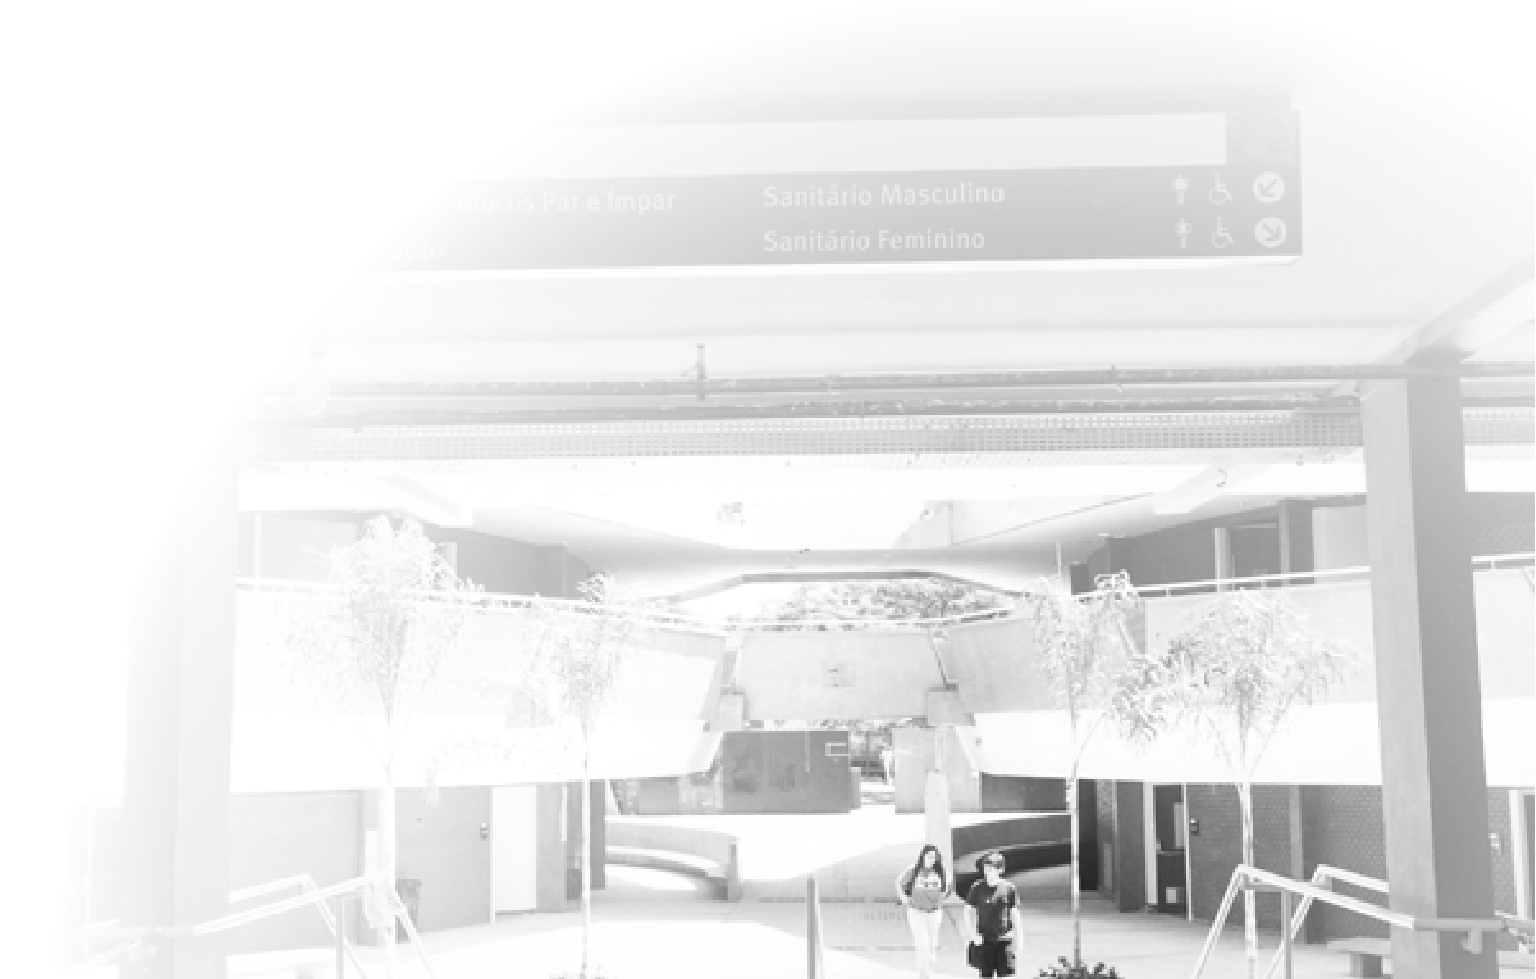
\includegraphics[scale=0.68, keepaspectratio=true]{img/imgs/1-boas_vindas/-007.jpg}
\end{figure}




\clearpage

\onecolumn

%%%%% Mensagem do diretor da FEEC
% Este arquivo .tex será incluído no arquivo .tex principal. Não é preciso
% declarar nenhum cabeçalho

\section{Mensagem do Diretor da FEEC}

Caros calouros de Engenharia de Computação,

É com grande satisfação que os recebemos na Unicamp e, em especial, na FEEC.
Nossa faculdade traz em sua denominação duas Engenharias de imensa importância:
Engenharia de Computação e Engenharia Elétrica.  O mundo moderno está assentado
sobre alguns pilares, dois destes são a Informação e a Energia.  E é exatamente
sobre nesses temas que a FEEC realiza suas atividades de ensino, pesquisa e
extensão há mais de 40 anos.  Ter os melhores cursos do Brasil é uma grande
responsabilidade. temos clareza de que isso foi construído por, principalmente,
contarmos com os melhores estudantes, ao que se associam excelentes professores
e uma infraestrutura que procura se manter renovada e atualizada.

Como vocês
experimentarão, Engenharia de Computação é um curso exigente, que requer
empenho e espera desempenho dos estudantes. Em contrapartida, vocês terão
oportunidade de participar da grande aventura do conhecimento, com descobertas,
talvez invenções, certamente com método.  Mas a Universidade é muito mais do
que o curso no qual vocês estão ingressando. É um mundo em si, com todas as
áreas do conhecimento, com convivência com pessoas dos mais diferentes lugares,
com arte e cultura, com debates e comemorações.  Aproveitem tudo isso, ao
máximo, sem esquecer que vocês estão em uma escola pública e gratuita, que sua
permanência aqui se deve ao trabalho de milhões de cidadãos do Brasil e, em
particular, de São Paulo. Honrem o trabalho de todas essas pessoas, dando o
melhor de si, com ética e dedicação, seja durante o curso, seja daqui a pouco,
quando já forem profissionais.

Bem-vindos à FEEC e a diretoria e as
coordenações de curso estarão sempre à disposição apra ajudar no que for
possível.


José Antenor Pomilio - Diretor da FEEC


\clearpage

%%%%% Mensagem do diretor do IC
% Este arquivo .tex será incluído no arquivo .tex principal. Não é preciso
% declarar nenhum cabeçalho

\section{Mensagem do IC}

Caros Alunos,

Sejam bem-vindos à Unicamp e ao Instituto de Computação (IC). 

Parabenizo a todos vocês pela conquista em estarem nesta instituição. No ano de
2014, o IC celebrou os 45 anos da Computação na Unicamp, um dos cursos mais
antigos do Brasil. Vale destacar que, desde sempre em sua trajetória, os nossos
cursos são reconhecidos dentre os melhores.  Trata-se de cursos de excelência
que reúnem com muita frequência os melhores alunos de várias escolas do Brasil e
que contam com professores com significativa atuação acadêmica e científica.

Neste momento se inicia uma nova etapa na vida de cada um: novo ambiente, novos
amigos, novos desafios, novas possibilidades; tudo isso acompanhado de mais
liberdade, independência e responsabilidade.  O ambiente universitário, vocês
verão, é extremamente fértil; oferece não apenas oportunidades acadêmicas de
qualidade (como aulas, palestras, mini-cursos, visitas técnicas e científicas,
estágios e atividades de iniciação científica), como também um universo de
experiências extracurriculares (Atlética, Centro Acadêmico, Bateria Valorosa,
Empresa Júnior, feiras de recrutamento, olimpíadas e maratonas de programação,
etc.) que possibilitam momentos inspiradores para aquisição de conhecimento,
maturidade e aperfeiçoamentos pessoal e profissional. Muitas destas atividades
extracurriculares são oferecidas ao mesmo tempo e não são raras as situações em
que conflitam com as atividades acadêmicas regulares. O principal desafio é
aprender a escolher e planejar, a gerenciar o tempo e os interesses, a cuidar
das relações pessoais, a considerar os prós e contras. Estejam atentos...

O que tenho para dizer a vocês, de ainda maior relevância, é algo que
erroneamente deixamos para o final da trajetória acadêmica quando, na verdade,
deveria ser a motivação de todas as nossas ações e que deveria permear todas as
nossas escolhas:

\begin{enumerate}
\item Sejam autores de suas próprias histórias;

\item Deixem vir à superfície a melhor versão de vocês mesmos;

\item Guiem-se pelos preceitos do Bem e do Belo e os defendam com a convicção de
  estarem colaborando pela alegria de se viver;

\item Não se acostumem nunca com aquilo que gostariam de mudar, com o que
  gostariam de romper, com o que lhes conduz para fora de seus caminhos no
  encontro consigo mesmos.
\end{enumerate}

Isso é o que devemos dizer para vocês, caros alunos, a todo instante durante
seus percursos nesses anos de universidade; é isso o que devemos dizer sempre a
nós mesmos enquanto docentes, orientadores, pesquisadores, cidadãos, enfim, como
pessoas. Proponho um desafio: que todos nós nos engajemos em perseguir e
converter em atos essas palavras; proponho que cada um de nós nos compromissamos
a transpor a preguiça, a desesperança, o medo, a incompreensão, a rivalidade sem
sentido, etc..., e busquemos realizar com responsabilidade o que nos faz
felizes, simplesmente. E que esse estado de contentamento irradie.

Parabéns a todos pela trajetória que se segue a partir daqui.

Ricardo da Silva Torres

Diretor,

Instituto de Computação,

Unicamp

\clearpage

\twocolumn

%%%%% Para pensar
% Este arquivo tex vai ser incluído no arquivo tex principal, não pe preciso
% declarar nenhum cabeçalho

\section{Para pensar}

O objetivo desse tópico não é responder grandes questões, nem doutrinar ninguém,
apenas expor alguns assuntos que achamos importante que você, bixo, analise
neste momento em que você está iniciando sua vida na universidade.

\subsection{UNICAMP, uma Universidade Pública?}

À primeira vista, um título como esse pode parecer estranho. "Mas como? Acabei
de entrar na UNICAMP, uma universidade estadual e não vou pagar mensalidades
para estudar nela. É óbvio que ela é uma Universidade Pública". Será?

Público, no sentido do dicionário, refere-se a "todos", ao "povo", mas também no
sentido popular quando nos referimos a algo público, logo lembramos de acesso
irrestrito e gratuito, sem distinção alguma a todos os cidadãos e cidadãs, um
lugar que todos tem direitos de usufruir. Mais ainda, público significa que
todos pagam, que é gerido e que foi construído com o dinheiro de todas as
pessoas através dos impostos arrecadados pelos mecanismos do Estado. É isso que
acontece por exemplo com os hospitais, creches e escolas públicas que, embora
possuam atendimento muitas vezes precário, atendem a todos.

Mas e uma universidade, de que forma ela se encaixa dentro do "público"?

Para responder melhor essa questão, devemos analisar a universidade com base em
seu tripé essencial: ensino, pesquisa e extensão. Comecemos por analisar
o acesso ao ensino. Por um lado, o processo seletivo da universidades públicas
paulistas, o vestibular, é uma forma virtualmente imparcial de seleção, que deve
analisar apenas o nível de conhecimento do candidato (que muitas vezes está
ligado ao valor de sua renda), sem levar em conta a religião, o sexo, ou
a classe social do vestibulando. Logo, exceto por pontos extras no vestibular
(para negros, índios e estudantes de escola pública), para ingressar em uma
universidade como a UNICAMP não há nenhuma distinção entre os cidadãos. Por
outro lado, só no Estado de São Paulo há cerca de 2 milhões de jovens com idade
para estar na universidade, enquanto isso as três universidades estaduais
paulistas (USP, UNESP e UNICAMP) não chegam a oferecer 100 mil vagas de
graduação e pós. Portanto, nem 5\% dos jovens paulistas tem acesso ao ensino
público superior, sendo que a grande maioria dos ingressantes na universidade
pública pertence às classes média ou alta. Existem iniciativas pontuais que
buscam mudar este quadro: Cursinhos comunitários (como a Cooperativa do Saber,
Cursinho do Sindicato, dentre outros) tem obtido um bom nível de aprovação de
seus alunos, porém em cursos com baixa concorrência, sendo que cursos como
medicina e computação continuam praticamente restritos às classe mais altas.

Agora, tendo em mente a pesquisa, podemos dizer que a UNICAMP se destaca nesse
ponto: Ela é responsável por 15\% de toda a pesquisa brasileira, desenvolve
vários estudos sobre a sociedade brasileira (tendo publicado recentemente um
atlas social), projetou equipamentos de segurança para carros, está trabalhando
em sistemas computacionais para saúde, entre tantas outras pesquisas voltadas
para o progresso da ciência e tecnologia nacional. Isso, sem contar que
a UNICAMP foi responsável por 35\% das patentes registradas na década de 90 aqui
no Brasil. Mas grande parte dessas patentes são vendidas a grandes empresas,
muitas vezes multinacionais. Outro ponto crítico existente são as pesquisas
particulares desenvolvidas na UNICAMP (a sala .NET, no IC, é um exemplo disso,
onde as patentes são divididas entre universidade, pesquisador e Microsoft).

Finalmente, falaremos sobre a extensão. Na nossa universidade o principal
projeto de extensão é a administração de hospitais da região, como o HC, que
é o maior hospital público do interior paulista, e atende pessoas de toda
a região e até de fora do Estado. Fora ele, a universidade não desenvolve nenhum
projeto de extensão gratuito que tenha grande destaque. No Instituto de
Computação, por exemplo, os cursos de extensão custam mais de R\$ 2000,00 por
aluno, o que não pode realmente ser chamado de extensão universitária, uma vez
que não está distribuindo à comunidade o conhecimento produzido aqui dentro.
Além disso a UNICAMP também restringe o acesso a diversos espaços da
universidade, como por exemplo o controle do acesso noturno ao campus,
a coibição de festas, e a dificuldade de acesso aos espaços da Faculdade de
Educação Física. Outras universidades como a UNESP e a USP Leste tem uma
política bem melhor de extensão. Na UNICAMP alguns alunos tem se dedicado
a desenvolver projetos de extensão que busquem a inclusão da comunidade na
universidade, através de cursinhos pré-vestibulares, reforço escolar,
e atividades com a população carente. A Computação historicamente tem pouco
engajamento, sendo que um dos únicos projetos com destaque é o GPSL, que
desenvolve a integração digital através do Software Livre, mas atualmente está
meio parado.

Resgatar o sentido do público tanto conceitual quanto materialmente se faz
sempre necessário. Assim, desde já, participe das discussões do centro acadêmico
para questionar as deficiências e produzir novos caminhos para formarmos com
a colaboração de todos uma universidade cada vez mais pública.

\subsection{Eu, um estudante público?}

Você já parou para pensar o que está começando ocorrer em sua vida? A partir de
agora você estuda em uma universidade pública, ou, como já foi dito, a partir de
agora o povo está pagando para você estudar. E o que você fará com esse
privilégio?

Se você for perguntar, encontrará milhares de maneiras de encarar o fato de ser
um estudante público, e provavelmente algumas das respostas provavelmente
incluiriam um pouco das visões a seguir:

Alguns veem a aprovação como o último passo do desafio de entrar na
universidade, uma conquista pessoal, e, desta maneira, a única pessoa a quem
estes tem de prestar contas sobre o que fizeram de seus estudos na UNICAMP
seriam eles mesmos. Outros acreditam que estudar em uma universidade pública
traz uma responsabilidade direta: estudar corretamente. Um aluno da UNICAMP
teria de aproveitar a universidade ao máximo, buscando sempre aprender, para que
saia daqui como um profissional competente para auxiliar o progresso tecnológico
da nossa sociedade, de modo a cumprir com o papel que lhe foi atribuído. Também
existem algumas pessoas que acreditam que assim que entramos na universidade nos
tornamos agentes públicos. Sendo assim, além de estudar também seria papel do
aluno interagir constantemente com a comunidade passando a ela os conhecimentos
que a universidade lhe proporcionou, buscando criar um elo
universidade-comunidade.

Afinal, qual dessas visões seria a mais correta sobre o que é um estudante
público? Essa é uma resposta que não daremos aqui (até porque, como foi dito no
início, respostas não fazem parte do objetivo deste tópico), ela é algo
individual. Mas seria bom que você pensasse qual a razão pela qual você está na
UNICAMP e qual o objetivo da sociedade quando ela paga para que você tenha essa
oportunidade.

E, bixo, nunca é demais desejar: Que você faça o melhor proveito do seu tempo
aqui na UNICAMP!


%%%%% Lugares para morar
% Este arquivo .tex será incluído no arquivo .tex principal. Não é preciso
% declarar nenhum cabeçalho

\section{Lugares para morar}

O preço de uma casa é a área do paralelepípedo formado pelos seguintes valores
nos eixos: proximidade da Unicamp, tamanho da casa (quantidade de quartos)
e qualidade da casa (acabamento, quantidade de banheiros, etc.) Quanto
à distância, a avenida 1 (avenida Dr. Romeu Tórtima) e avenida 2 (avenida Prof.
Atílio Martini) são bem caras por serem próximas da Unicamp, as ruas entre elas
muitas vezes também são. A região que vai do centro de Barão até a moradia
geralmente é boa e barata para se morar: Tem bastantes serviços e ainda é perto
da Unicamp (mais ou menos 10 minutos de bicicleta).

Uma boa dica para se informar a respeito de lugares para morar (repúblicas,
kitnets, pensões) é o site Morar Unicamp
(\url{www.morarunicamp.com.br}), criado por alunos da Unicamp e que
contém informações como endereço, preço, contato e detalhamento do lugar. E mais
lugares podem ser adicionados ao site.

\subsection{Moradia Estudantil}

A moradia estudantil é um exemplo de conquista de todos os estudantes.
O processo de reivindicação de uma moradia estudantil para a Unicamp começou com
o movimento TABA. Durante muito tempo, alunos ficaram acampados no CB (Ciclo
Básico) para reivindicar seu direito a estudar. Hoje em dia, graças à moradia,
várias pessoas que possivelmente não teriam condições de se manter em Campinas
pagando aluguel, tem como estudar na Unicamp. A moradia existe desde 1989
e durante esse período a Unicamp ampliou muito suas vagas. Isto fez as vagas na
moradias tornarem-se insuficientes para todos que querem. Alguns anos atrás
houve grandes movimentações pela ampliação e reforma da moradia, pois algumas
casas estavam caindo.

Cada "casa" (que normalmente é dividida entre quatro pessoas) se constitui de um
quarto, uma cozinha, um banheiro e uma sala. Ainda tem o Circular da Moradia, um
ônibus da Unicamp que transporta a galera durante o dia todo da moradia até
a Unicamp e vice-versa.

A moradia está localizada na Avenida Santa Isabel, 1125. Aproximadamente a uns
3 km do campus da Unicamp.

Para saber mais sobre o processo seletivo entre no site da Moradia Estudantil
(\url{www.pme.unicamp.br}). Muito provavelmente você
será abordado por um assistente social na matrícula.

\subsection{Repúblicas}

Geralmente a melhor escolha, se você tiver condições de pagar por uma moradia.
Você pode levar quem quiser para sua casa (dependendo da aprovação dos
moradores), chegar no horário que quiser, e conhecerá muita gente nova. Tente,
se possível, morar em uma república de cursos mistos, pois assim você terá
contatos diversos. O custo de uma vaga em uma república é muito variável
(depende do nível de conforto que você quer). Gira em torno de
R\$350,00 o aluguel para dividir quarto e R\$450,00 para pegar
um quarto sozinho, além das contas adicionais (água, luz, etc.), que costumam
totalizar R\$150,00, em média. Procure bem as pessoas com quem você vai morar para não ter
problemas com diferentes estilos de vida (tem gente que gosta de lavar louça
a cada 5 minutos e tem gente que gostaria de morar junto com porcos, veja com
quem você se dá melhor).

\subsection{Kitnets}

Tomem cuidado com elas, pois a especulação imobiliária em Barão Geraldo chega
a ser imbecil. E nos últimos anos ficou fora de controle. As kitnets mobiliadas,
normalmente um quarto-sala-cozinha-área de serviço e banheiro, estão com valores
da ordem de R\$ 1000,00 para mais. Sim, mil reais por um microespaço. Só porque
é perto da Unicamp. Fique de olho e tome cuidado com os contratos.

As melhores relações custo-benefício de kitnets são aquelas próximas ao centro
de Barão Geraldo ou no espaço entre as avenidas. E lembre-se não é só de Unicamp
que se vive. Não adianta pagar mais caro para estar do lado da Unicamp, se você
fica muito longe dos mercados, farmácias etc.

\subsection{Pensões}

Dependendo da pensão que você conseguir pode tornar-se uma grande roubada.
Algumas pensões não deixam você levar pessoas para sua casa, reclamam se você
chegar tarde e não liberam festas, já outras não; então procure bem. O preço
também não é muito bom, mas costuma ser mais barato que kitnets. É bom se você
quer um esquema casa-comida-roupa-lavada. É muito importante que você saiba que
contratos de um ano (ou qualquer período) em pensionatos são ilegais e você não
precisa cumpri-los.

\subsection{Dicas de Segurança}

Além de um novo ambiente de estudos, conhecerá novos lugares e pessoas. E,
provavelmente, em breve estará planejando sua mudança para Campinas.

Muitos dos estudantes moram em Barão Geraldo, por ser mais perto da Unicamp,
possibilitando que sua bicicleta se torne seu meio de transporte principal, por
ser o lugar com maior número de repúblicas e pensionatos e também por ser onde
a maior parte das festas acontece!

No entanto, por ser constituído em sua maioria por casas de famílias com muitas
posses e casas de estudantes (em geral desatentos), Barão Geraldo peca pela
falta de segurança.

Não é raro ouvir de alguém que foi assaltado enquanto voltava para casa à noite
sozinho ou que a casa foi saqueada durante um feriado prolongado. Portanto,
é importante zelar pela sua integridade e de seus pertences -- assim como seus
pais fazem em sua casa, não importa onde eles morem.

Se sua pensão ou república paga o segurança da rua, faça uso dele, seja pedindo
escolta ao chegar em casa ou telefonando caso ouça algum barulho suspeito. Ao
voltar para sua cidade em feriados prolongados, deixando a casa vazia, não se
esqueça de trancar todas as portas e janelas de casa, verificar se não há nada
no quintal que possa ser levado facilmente (colocar as bicicletas e aparelhos de
som na sala pode ser uma boa ideia), e trancar os objetos de valor
(computadores, televisões) nos quartos.

\subsection{Imobiliárias}

\begin{itemize}
\item  \textbf{Imobiliária Barão Housing}
\begin{itemize}
\item  Telefone: (19)3289-4113.
\item  Endereço: Rua Tranquilo Prosperi, 383 -- Jd. Sta. Genebra II.
\item  E-mail: atendimento [@] baraohousing [.] com[.] br.
\item  Site: \url{www.baraohousing.com.br}
\end{itemize}
\end{itemize}

\begin{itemize}
\item  \textbf{Imobiliária Home Hunters}
\begin{itemize}
\item  Endereço: Rua Benedito Alves Aranha, 55.
\item  Telefone: (19) 3289-0044.
\item  E-mail: bgeraldo [@] homehunters [.] com [.] br.
\item  Site: \url{www.homehunters.com.br}
\end{itemize}
\end{itemize}

\begin{itemize}
\item  \textbf{Imobiliária Barão Geraldo}
\begin{itemize}
\item  Endereço: Aavenida Dr. Romeu Tórtima, 183.
\item  Telefone: (19) 3289-2315.
\item  E-mail: atendimento [@] imobiliariabaraogeraldo [.] com [.] br.
\item  Site: \url{www.imobiliariabaraogeraldo.com.br}
\end{itemize}
\end{itemize}

\begin{itemize}
\item  \textbf{Imobiliária Lanza}
\begin{itemize}
\item  Endereço: Rua Benedito Alves Aranha, 104.
\item  Telefone: (19) 3289-1717.
\item  E-mail: lanza [@] lanzaimoveis [.] com [.] br.
\item  Site: \url{www.lanzaimoveis.com.br}
\end{itemize}
\end{itemize}

\begin{itemize}
\item  \textbf{Imobiliária Professor Sebastião}
\begin{itemize}
\item  Endereço: Avenida Dr. Romeu Tórtima, 344.
\item  Telefone: (19) 3289-2317.
\item  E-mail: ipsimoveis [@] ipsimoveis[.] com [.] br.
\item  Site: \url{www.ipsimoveis.com.br}
\end{itemize}
\end{itemize}

\begin{itemize}
\item  \textbf{Amaral Imóveis}
\begin{itemize}
\item  Endereço: Avenida Dr. Luiz de Tella, 864.
\item  Telefone: (19) 3287-5255.
\item  E-mail: amaral [@] amaralimoveis [.] net.
\item  Site: \url{www.amaralimoveis.net/}
\end{itemize}
\end{itemize}

\begin{itemize}
\item  \textbf{Zaine Conquista Imóveis}
\begin{itemize}
\item  Endereço: Avenida Santa Izabel, 84.
\item  Telefone: (19)3289-4050.
\item  E-mail: zaine [@] correionet [.] com [.] br.
\item  Site: \url{www.zaineconquista.com.br}
\end{itemize}
\end{itemize}

\begin{itemize}
\item  \textbf{W. Post Imóveis}
\begin{itemize}
\item  Endereço: Avenida Dr. Romeu Tórtima, 1140.
\item  Telefone: (19) 3289-2155.
\item  E-mail: w.post [@] ig [.] com [.] br.
\item  Site: \url{www.wpostimoveis.com.br}
\end{itemize}
\end{itemize}

\begin{itemize}
\item  \textbf{Ismê Assessoria Imobiliária}
\begin{itemize}
\item  Endereço: Rua Christina G. Miguel, 250.
\item  Telefone: (19) 3289-4325.
\item  E-mail: isme [@] isme [.] com [.] br.
\item  Site: \url{www.isme.com.br}
\end{itemize}
\end{itemize}

\begin{itemize}
\item  \textbf{Rute Svartman Imóveis}
\begin{itemize}
\item  Telefone: (19) 3287-4641
\item  E-mail: imoveis [@] rutesvartman [.] com[.] br
\item  Site: \url{www.rutesvartman.com.br}
\end{itemize}
\end{itemize}

\begin{itemize}
\item  \textbf{Imobiliária Ávila \& Ferraris}
\begin{itemize}
\item  Endereço: Avenida Dr. Romeu Tortima, 714
\item  Telefone: (19) 3289-4468
\item  E-mail: dcaavila [@] terra [.] com [.] br
\item  Site: \url{www.avilaeferrarisimoveis.com.br}
\end{itemize}
\end{itemize}

\begin{itemize}
\item  \textbf{Imobiliária Cidade Universitária}
\begin{itemize}
\item  Endereço: Avenida Dr. Romeu Tortima, 624.
\item  Telefone: (19) 3289-3322.
\item  E-mail: contato [@] cidadeuniversitariaimoveis [.] com [.] br.
\item  Site: \url{www.cidadeuniversitariaimoveis.com.br}
\end{itemize}
\end{itemize}

\begin{itemize}
\item  \textbf{Denilson Imóveis}
\begin{itemize}
\item  Endereço: Avenida Dr. Luís de Tella, 55.
\item  Telefone: (19) 3289-1444.
\item  E-mail: denilsonimoveis [@] terra [.] com [.] br.
\end{itemize}
\end{itemize}

\begin{itemize}
\item  \textbf{Mega Barão Imóveis}.
\begin{itemize}
\item  Endereço: Rua Francisca Resende Merciai, 103.
\item  Telefone: (19) 3289-7101.
\item  E-mail: megabarao [@] megabaraoimoveis [.] com [.] br.
\item  Site: \url{www.megabaraoimoveis.com.br}
\end{itemize}
\end{itemize}

\begin{itemize}
\item  \textbf{Libano Imóveis}
\begin{itemize}
\item  Endereço: Rua Francisca Resende Merciai, 112.
\item  Telefone: (19) 3289-0441.
\item  E-mail: contato [@] libanoimoveis [.] com [.] br.
\item  Site: \url{www.libanoimoveis.com.br}
\end{itemize}
\end{itemize}

\begin{itemize}
\item  \textbf{Marco Imóveis}.
\begin{itemize}
\item  Endereço: Rua José Pugliesi Filho, 420 -- Guará.
\item  Site: \url{www.marcoimovel.com.br}
\end{itemize}
\end{itemize}

\begin{itemize}
\item  \textbf{Imobiliária Canal}
\begin{itemize}
\item  Endereço: Avenida Professora Ana Maria Silvestre Adade, 555.
\item  Telefone: (19) 3256-2622.
\end{itemize}
\end{itemize}

\begin{itemize}
\item  \textbf{Lokal Imóveis}
\begin{itemize}
\item  Endereço: Rua José Próspero Jacobucci, 290.
\item  Telefone: (19) 3256-4616.
\end{itemize}
\end{itemize}

\begin{itemize}
\item  \textbf{Esparta Empreendimentos Imobiliários}
\begin{itemize}
\item  Endereço: Avenida Albino José Barbosa de Oliveira, 830.
\item  Telefone: (19) 3289-5353.
\end{itemize}
\end{itemize}

\begin{itemize}
\item  \textbf{Cássio Carvalho Imóveis}
\begin{itemize}
\item  Endereço: Avenida Santa Isabel, 750.
\item  Telefone: (19) 3288-0144.
\item  E-mail: cassio [@] cassioimoveis [.] com [.] br.
\item  Site: \url{www.cassioimoveis.com.br}
\end{itemize}
\end{itemize}

\begin{itemize}
\item  \textbf{Roma Imóveis}
\begin{itemize}
\item  Endereço: Rua Agostinho Pattaro, 222.
\item  Telefone: (19) 3289-0441.
\end{itemize}
\end{itemize}

\begin{itemize}
\item  \textbf{Valter Imóveis}
\begin{itemize}
\item  Endereço: Rua Maria Ferreira Antunes, 22.
\item  Telefone: (19) 3289-6088.
\end{itemize}
\end{itemize}

\begin{itemize}
\item  \textbf{Imobiliária Marco Antônio}
\begin{itemize}
\item  Endereço: Avenida Dr. Romeu Tórtima, 1522.
\item  Telefone: (19) 3289-2417.
\end{itemize}
\end{itemize}

\begin{itemize}
\item  \textbf{André Imóveis}
\begin{itemize}
\item  Endereço: Rua Maria Nassif Mokarzel, 42.
\item  Telefone: (19) 3289-6607.
\end{itemize}
\end{itemize}

\begin{itemize}
\item  \textbf{VPR Imóveis}
\begin{itemize}
\item  Endereço: Av. Professor Mário Werneck, 2011.
\item  Telefone: (19) 3289-6607.
\item  Site: \url{www.vprimoveis.com.br}
\end{itemize}
\end{itemize}


%%%%% Comida
% Este arquivo tex vai ser incluído no arquivo tex principal, não pe preciso
% declarar nenhum cabeçalho

\section{Comida}
\subsection{Bandejão}

Um dos momentos de glória do dia de um futuro engenheiro, cientista ou bacharel
é o bandejão. É a hora de intensas e indiscutíveis emoções. Caso sua salada
corra sobre a mesa, mantenha-se calmo. Evite discussões, jamais tente descobrir
o sabor do suco pelo paladar (limão ou pêssego?) é mais cômodo ler no cardápio
do dia. Uma dica: para cortar o bife faça muita força e quando começar
a amolecer pare, você chegou na bandeja.

Falando sério agora: O bandejão (Restaurante Universitário), Bandex, ou Bandeco,
fica ao lado da Biblioteca Central, bem em frente ao PB (Prédio Básico, ou Ciclo
Básico II) e, a menos que você não queira economizar uma boa grana com comida,
vai ser o lugar onde você vai estar na maioria dos seus horários de almoço. Com
o tempo, você vai ver que o Bandex é o "coração da UNICAMP": É o local de você
se encontrar com os amigos (combinando ou não antes), contar os micos nas aulas,
jogar conversa fora, e falar mal da comida, que nem é tão ruim assim como muitos
dizem. Sem dúvida, é o melhor custo-benefício da UNICAMP: Por R\$2,00, você tem
direito a arroz, feijão, salada, proteína de soja, suco, chá e café à vontade,
a carne e a sobremesa tem que dar uma choradinha para a tiazinha para poder
repetir, mas geralmente dá certo.

Existe também o RA (Restaurante Administrativo), também conhecido como Pratex,
pelo fato da comida ser servida em pratos e não em bandejas. Fica atrás da
Faculdade de Engenharia Elétrica e de Computação (FEEC), perto do prédio da Engenharia Básica. Tem algumas diferenças em
relação ao Bandex: O espaço físico é bem menor, por exemplo. No RA você mesmo se
serve, apesar da carne às vezes ser servida pela tia que trabalha lá. Se você
for com um amigo, vá com paciência para esperar, porque é difícil pra arrumar
lugar, além ser ultra apertado. Dependendo de onde você vai ter aula antes ou
depois do almoço, é mais negócio almoçar no Pratex. Para poder usar o Bandex
e o RA, você deve estar com o seu cartão (C.U.) carregado.

Nota: se vocês derem sorte, pode ser que o novo Pratex já esteja pronto e tenha
sido aberto. Ele é localizado próximo ao IC3 e ao prédio azul da Civil.

\subsubsection{Como funciona o esquema de carregar o cartão?}

Simples. Você vai ao guichê ao lado esquerdo da entrada do Bandex, e faz, por
exemplo, um depósito de R\$20,00 para 10 créditos. Outra maneira de colocar
créditos no C.U. é fazer um depósito na conta do Bandex no Banespa (Ag.: 207
/ Conta: 43.010.009-2) ou no Banco do Brasil (Ag.: 4203-X / Conta: 66.315-8)
e depois carregar o seu cartão, no guichê do Bandex ou na Prefeitura do Campus
(próximo à Reitoria). Fique esperto para não ir ao RA sem créditos, porque lá
não dá pra carregar o cartão e você terá que andar até o Bandeco.

Os bandejões funcionam de segunda a sexta, nos seguintes horários:

\begin{itemize}
\item  RU, das 10h30 às 14h00 (almoço) e das 17h30 às 19h40 (jantar).
\item  RA, das 11h30 às 14h00 (almoço) e das 17h30 às 19h00 (jantar).
\end{itemize}
Para saber previamente o cardápio do Bandejão, acesse o site do CACo (\url{http://www.caco.ic.unicamp.br}).

Uma opção para consultar o cardápio do bandejão é o bandecowap. Ele foi feito
pensando na possibilidade de consultar o cardápio através do telefone celular,
mesmo aqueles mais simples que oferecem acesso à internet mais básico, na forma
de WAP. Há também a possibilidade de instalar um gadget na página inicial do
Google, a iGoogle. Acesse pelo \url{www.tinyurl.com/bandecowap} ou, se preferir
adicionar aos favoritos, use o \url{www.students.ic.unicamp.br/~ra092856/bandecowap}
- o acesso por este é ligeiramente mais rápido, pois não há o redirecionamento.

\subsection{Outros lugares para as refeições}

Lugares que servem pratos feitos são a Física (um os melhores da UNICAMP, serve
também meio-prato), o IFCH (a comida lá é bem barata) e a Química (bem parecido
com o da Física).

A cantina do DCE tem self-service barato e com variedade no almoço. Outros
lugares que tem self-service são a Artes, a Educação, a Física e a Mecânica.

Se você é vegetariano, uma boa dica é o Gatti (que fica do lado do IC-2, na
Cênicas/Dança).

Fora da Unicamp: próximo ao balão da Av. 1, temos também o Terraço, que vende
marmitex e tem self-service a um preço bom, além de churrasco às terças, quintas
e sábados. Um pouco mais acima na Av. 1, tem o Bardana (um com a fachada toda
verde), que está na mesma faixa de preço do Terraço, e costuma ser considerado
bem melhor; tem churrasco de carne bovina meio que dia-sim-dia-não, e nos outros
dias é de frango. Próximo ao Bardana, tem o Pepe Loco, que serve comida mexicana
no estilo fast-food. Na frente da reitoria há o Del Sol, o Ginza e o Moriá.
O Del Sol serve comida por quilo, sendo parecido (em preço e pratos) com
o Bardana, enquanto que o Ginza serve a la carte com preços bons (uma dica
é a feijoada completa às quartas, que sai por R\$10,00 e inclui uma
mini-capirinha!) e o Moriá serve pratos feitos a preços mais baratos. Próximo ao
Ginza, em frente à guarita do HC, há o Campus Grill, com comida boa a um preço
um tanto alto (um pouco mais caro que a cantina da Física). Tem o Aulus, na Av.
2, próximo ao balão, que é o mais caro dos citados aqui, mas é muito bom (e
bonito).

\subsection{Lanches e sucos}

Tá de tarde, bateu fome, quer comer um lanche (hamburger, pão-na-chapa, queijo
quente, x-salada, croissant, qualquer coisa do gênero)? Quase todas as cantinas
da UNICAMP servem lanche. Algumas muito boas são o IFCH, a Física, a lanchonete
do IEL e a lanchonete da Economia.

Quase todas as cantinas servem salgados prontos, lanches naturais, doces
e demais coisas do gênero.

Para sucos, tem dois lugares muito bons: a cantina da Física e a famosíssima
banca de sucos do CB, que tem milhões de sucos, vende frutas e também salgados.
Se você precisa almoçar rápido, provavelmente sua escolha será salgado
+ vitamina na banca de sucos do CB. Todo dia a banca de sucos do CB tem um sabor
na oferta, que é ótimo pra sair do tradicional suco de laranja.

Açaí: a cantina da física tem um açaí na tigela, caro, mas bom. Se por algum
motivo você tiver de andar até o quarteirão de salas de aula da medicina,
estiver cansado, e quiser um açaí, o da cantina de lá é caro
e inacreditavelmente zoado.

Nas quartas-feiras há uma feira no centro da praça do CB, na qual há opções bem
variadas, desde pastéis a comida japonesa, embora geralmente mais caras que as
cantinas. Algumas das barracas abrem também na quinta-feira.

\subsection{Padarias e café da manhã}

Cinco cantinas da UNICAMP abrem bem cedo e servem o bom pingado + pão na chapa
matinal. São elas a Mecânica, a cantina do IFCH, a cantina do DCE, a da Química
e a da Física.

A Padaria Alemã serve uma bandeja de café da manhã com suco,
café-com-leite/chocolate, croissant, mamão, bolo, pão francês, torradas,
manteiga e geléia. Ainda há a possibilidade de fazer trocas como: suco por
chocolate, croissant por dois pães-na-chapa, mamão por banana, coisas do gênero.
Também são servidos lanches gigantescos, com muitas opções de recheio, por um
preço relativamente barato, então tenha alguém para dividir (acredite, meio
lanche já serve como um almoço completo). Dependendo do recheio, a pizza é muito
barata, também, embora eles não façam delivery. A Alemã fica na Avenida 1 (a da
saída da FEEC). É bom lembrar que eles servem café-da-manhã das 7h até às 13h
(mas a padaria só fecha às 22h), então é uma boa pedida para se você não quiser
almoçar ou para sábado e domingo, acordar tarde e tomar um café da manhã para
valer pelo almoço.

Na Estrada da Rhodia, próximo à entrada da Cidade Universitária II, há
a Paneteria Di Capri, que tem um pão francês muito bom (a um preço legal)
e também muita variedade (incluindo tortas e lanches). Além disso você também
pode tomar seu café da manhã lá, pois como quase toda padaria eles também
oferecem um cardápio bom para logo cedo. Se você estiver com bastante apetite,
de sexta a domingo eles servem um buffet de café-da-manhã com muitas opções
e a um preço fixo (em torno de R\$10). Na hora do almoço também são preparados
alguns pratos (para comer no local e para levar) e também há um esquema onde
você pede um grelhado e tem acesso livre a um balcão com saladas e outras
coisas, como petiscos. À noite eles servem pizzas e também há o esquema do
grelhado, exceto no inverno, quando eles servem um buffet de sopas.

Já se você está na Unicamp e quer uma padaria, a dica é a Padaria da FEA (fica
próxima à Cantina da Mecânica). Lá eles tem pães, doces e bolos. Com uma
diferença: há produtos especiais, como pão de queijo com linhaça ou alho e pão
francês com soja. Mas não se assuste: por mais estranho que pareçam, os produtos
de lá são muito bons! E não deixe para ir lá depois das aulas, pois a Padaria da
FEA fecha às 17h.

\subsection{E no fim de semana?}

Nos fins de semana, nem o Bandex nem quase nenhuma cantina da Unicamp abrem (e
as que abrem só o fazem no sábado). Você vai ter que se virar fora da Unicamp.
Na Av. 1 e proximidades tem o Terraço, o Bardana e a Padaria Alemã já citados,
o Lilly (que assim como o Terraço e o Bardana não abre de domingo), além de
vários restaurantes próximos à Alemã. Na Av. 2 tem o Aulus (mais caro no sábado
que durante a semana; domingo, então, mais ainda, mas costuma ter camarão
à milanesa), o Clos Vert (também é caro), um pouco mais pra cima na avenida e,
pouco depois, há o Yaki-Ten, que serve comida chinesa por quilo e japonesa por
pessoa. Logo mais abaixo há o Ilha do Barão. No centro de Barão não faltam
opções. Tem (indo da entrada de Barão pela Estrada da Rhodia) o Estância Grill,
o Barão da Picanha, o Gordão Burguers, o Solar dos Pampas, o Universo Massas,
o Vila Santo Antonio, o Ki-Pizza, o restaurante Baroneza, o Salsinha
e Cebolinha, o Pão de Açúcar e vários restaurantes no Tilli Center (a dica
é o Subway, por menos de 10 reais você come bem). Na Av. Santa Isabel
e adjacências tem o Cronópio (numa rua paralela à Santa Isabel), o Frangonete
(próximo ao Banespa), o HotDog Central e as Pizzarias Sapore Pizza e Pizza
Fiori. Perto da moradia tem a Tonha (Canto do Acarajé), o Kalunga Lanches
e o famoso dogão da moradia. Por fim, próximo à padaria Di Capri, há alguns
restaurantes mais caros, como a Romana (serviço parecido com o da Di Capri,
porém um bocado mais cara), Pizzaria Gregória, o TBONE (eles também tem
marmitex), o Greg Burgers (o hambúrguer e o milk-shake são excelentes), o Tábua
dos Mares e o Morena-flor.

\subsubsection{Alguns telefones:}

\begin{itemize}
\item  \textbf{Restaurante Baroneza}
\\\underline{Telefone:} (19) 3289-9087.
\\\underline{Endereço:} Rua Benedito Alves Aranha, 44 -- Centro de Barão Geraldo.
\\\underline{Site:} \url{http://www.restaurantebaronesa.embarao.com/}
\end{itemize}

\begin{itemize}
\item  \textbf{China In Box} (Faz entrega em Barão)
\\\underline{Telefone:} (19) 3254-5601
\\\underline{Endereço:} Rua Romualdo Andreazzi, 333 -- Jd. Trevo.
\end{itemize}

\begin{itemize}
\item  \textbf{TBONE Steak Bar}
\\\underline{Telefone:} (19) 3289-0485.
\\\underline{Endereço:} Rua Maria Tereza Dias da Silva, 700.
\end{itemize}
\end{itemize}

\begin{itemize}
\item  \textbf{Habibs} (Não está mais entregando em Barão)
\\\underline{Telefone:} 0800-778-2828
\end{itemize}

\begin{itemize}
\item  \textbf{Ginza Bar}
\\\underline{Telefone:} (19)3289-9281
\\\underline{Endereço:} Rua Roxo Moreira, 1768.
\end{itemize}
\end{itemize}

\begin{itemize}
\item  \textbf{Bardana}
\\\underline{Telefone:} (19)3289-9073.
\\\underline{Endereço:} Avenida Dr. Romeu Tórtima, 1500.
\end{itemize}

\begin{itemize}
\item  \textbf{Terraço}
\\\underline{Telefone:} (19) 3289-7920
\\\underline{Endereço:} Rua Roxo Moreira, 1344
\end{itemize}

\begin{itemize}
\item  \textbf{Pastelaria Oba-Oba}
\\\underline{Telefone:} (19) 3249-1908
\\\underline{Endereço:} Rua Benedito Alves Aranha, 115
\end{itemize}

\begin{itemize}
\item  \textbf{Estância Grill}
\\\underline{Telefone:} (19) 3289-6055
\\\underline{Endereço:} Avenida Albino José Barbosa de Oliveira, 271
\end{itemize}

\begin{itemize}
\item  \textbf{Pizzaria Borda de Ouro.}
\\\underline{Telefone:} (19) 3289-0867.
\\\underline{Endereço:} Luiz Vicentin Sobrinho, 457.
\end{itemize}

\begin{itemize}
\item  \textbf{Barão das Pizzas.}
\\\underline{Telefone:} (19) 3249-1630.
\\\underline{Endereço:} Rua Agostinho Pattaro, 187.
\end{itemize}

\begin{itemize}
\item  \textbf{Pizza Fiori.}
\\\underline{Telefone:} (19) 3289-3514.
\\\underline{Endereço:} Avenida Santa Isabel, 405.
\end{itemize}

\begin{itemize}
\item  \textbf{Ki-Pizza.}
\\\underline{Telefone:} (19) 3289-0863.
\\\underline{Endereço:} Rua Horácio Leonardi, 76.
\end{itemize}

\begin{itemize}
\item  \textbf{Bella Pizza.}
\\\underline{Telefone:} (19) 3289-7777.
\end{itemize}

\begin{itemize}
\item  \textbf{Pizza Show}
\\\underline{Telefone:} (19) 3324-7480
\end{itemize}

\begin{itemize}
\item  \textbf{Quero Mais.}
\\\underline{Telefone:} (19) 3289-4072.
\end{itemize}

\begin{itemize}
\item  \textbf{Estação Santa Fe Pizza.}
\\\underline{Telefone:} (19) 3289-4800.
\end{itemize}

\begin{itemize}
\item  \textbf{Pizza Gigante (Mega Pizza).}
\\\underline{Telefone:} (19) 3289-0320.
\end{itemize}

\begin{itemize}
\item  \textbf{Vila Ré Pizza.}
\\\underline{Telefone:} (19) 3289-0321.
\end{itemize}

\begin{itemize}
\item  \textbf{NADOG'S -- HOT DOG DO NADO}
\\\underline{Telefone:} (19) 3029-2270.
\end{itemize}

\begin{itemize}
\item  \textbf{Casa da Moqueca} (prato mais caro, mas serve duas pessoas)
\\\underline{Telefone:} (19) 3289-3131.
\end{itemize}

\subsection{E de madrugada?}
\begin{itemize}
\item  \textbf{Rob's Burgers:} (entregas até as 23:30).
\begin{itemize}
\item  Telefone: (19)3289-6541.
\item  Endereço: Avenida Santa Isabel 1510 (em frente ao portao 2 da moradia da UNICAMP).
\item  Tem vários tipos de lanches, não cobram taxa de entrega e é aberto das 18:30 as 23:30. E para quem estiver com muita fome tem o x-especial que é grande e muito bom.
\end{itemize}
\end{itemize}

\begin{itemize}
\item  \textbf{Hot-dog Independência:}
\begin{itemize}
\item  Telefone: (19)3289-8805
\item  Endereço: Rua Angela Signol Grigol, 742
\item  Tem vários tipos de hot-dogs (com catupiry, com cheddar, com frango{\dots}) e tem preços menores que os do Rod Burguers. O único problema é que eles cobram taxa de entrega para um lanche e fecham à meia-noite.
\end{itemize}
\end{itemize}

\begin{itemize}
\item  \textbf{Kalunga Lanches:}
\begin{itemize}
\item  Telefone: (19)3289-5236
\item  Endereço: Rua Sebastião Bonomi, 40
\item  Perto da moradia, eles não entregam, mas ficam abertos até altas horas. Destaque para o caldinho de feijão. Obs: o lugar é limpo e bom.
\end{itemize}
\end{itemize}

\begin{itemize}
\item  \textbf{Ponto Final:}
\begin{itemize}
\item  Telefone: (19) 3288-0204.
\item  Endereço: Avenida Albino José Barbosa de Oliveira, 2287
\item  Lanchonete localizada na estrada da Rhodia e entrega lanches até a meia noite. Tem tradição de ter preços caros, por isso não se estranhe. Muitos gostam bastante dessa lanchonete pela famosa maionese temperada que eles servem, não se esqueça de pedir quando for comprar lanches.
\end{itemize}
\end{itemize}

\begin{itemize}
\item  \textbf{Gordão:}
\begin{itemize}
\item  Telefone: (19)3289-9753
\item  Endereço: Avenida Albino José Barbosa de Oliveira, 476
\item  Rua Localizada na entrada de Barão Geraldo servem lanches parecidos com o do Ponto Final, lá eles dão outro tipo de maionese e em geral os preços são tão caros quanto do Ponto Final. Também entregam até meia noite.
\end{itemize}
\end{itemize}

\begin{itemize}
\item  \textbf{Lanchão \& Cia:}
\begin{itemize}
\item  Telefone: (19)3289-3665
\item  Endereço: Avenida Albino José Barbosa de Oliveira, 1214
\item  Site: \url{http://www.lanchaoecia.com.br/}
\item  (Fechou, abriu um novo barzinho no lugar em Barão). Um dos melhores lanches de Campinas (quiçá o melhor). Os lanches geralmente são grandes e muito bons, e os preços são compatíveis com a qualidade e quantidade. Eles servem no carro se você preferir, com uma bandeja que fica presa no vidro. Fica no centro de Barão Geraldo, proximo ao Banespa e Pão de Açucar. Destaque para a batata frita, feita de uma forma muito diferente, extremamente crocante e quase cremosa por dentro. Há outras duas lojas próximas da avenida Norte-Sul. Uma na Rua Oriente, e outra na Orozimbo Maia. O Art Lanches (antigo Lanchão 2), que fica no Taquaral, serve lanches parecidos.
\end{itemize}
\end{itemize}

\begin{itemize}
\item  \textbf{Ponto 1:}
\begin{itemize}
\item  Telefone: (19)3289-2378.
\item  Rua Eduardo Modesto, 54
\end{itemize}
\end{itemize}

\begin{itemize}
\item  \textbf{Sapore Pizza:}
\begin{itemize}
\item  Telefone: (19)3289-0228
\item  Endereço: Avenida Santa Isabel, 326
\item  Para quando você estiver com pelo menos mais um amigo para rachar a pizza, acaba sendo uma boa pedida. Geralmente as pizzas de mussarela e de calabreza estão com preços bem acessíveis. Também entregam até meia-noite.
\end{itemize}
\end{itemize}

\begin{itemize}
\item  \textbf{Barraquinhas:}
\begin{itemize}
\item  Há várias barraquinhas de hot-dog no centro de Barão e perto da moradia. Destaque para o dog do terminal, o Hot Dog Central, o Pedrogue e o dogão da moradia. Se você quiser um lanche, uma boa pedida é o Star Trash (Raimundão ou Guarujá, chame como você quiser), que fica perto do balão da avenida 2 e costuma ficar aberto até altas horas. Perto da UNICAMP, ao lado do posto Ipiranga que fica na avenida 1 também tem um dog prensado muito bom e barato.
\end{itemize}
\end{itemize}

\subsection{Marmitex}

Entrega em casa. Bom e barato.

\begin{itemize}
\item  \textbf{Tia Rita.}
\begin{itemize}
\item  Telefone: (19) 3249-2899.
\end{itemize}
\end{itemize}

\begin{itemize}
\item  \textbf{Hailton}
\begin{itemize}
\item  Telefone: (19) 3249-0153.
\end{itemize}
\end{itemize}

\begin{itemize}
\item  \textbf{Copa e Cozinha}
\begin{itemize}
\item  Telefone: (19) 3249-0153.
\end{itemize}
\end{itemize}

\begin{itemize}
\item  \textbf{Império do Barão}
\begin{itemize}
\item  Telefones: (19) 3289-8054 e (19) 3289-2170.
\end{itemize}
\end{itemize}

Obs: A Sapore Pizza também entrega Marmitex.

\subsection{Bares, lanchonetes e restaurantes}
\begin{itemize}
\item  \textbf{Açaizeiro Brasil:} Serve um açaí muito bom e vários tipos de comidas mais leves, como lanches naturais, crepes e saladas, além de vários sucos. O preço não é caro e a comida é boa. Endereço: Avenida Santa Isabel, 518. Telefone: (19) 3365-6555. Site: \url{http://www.portalbaraogeraldo.com.br/anunciantes/acaizeiro-brasil/}
\end{itemize}

\begin{itemize}
\item  \textbf{Alkobar:} Comida árabe e pizzas no início da Santa Isabel. Bom atendimento, comida legal e preço razoável. Telefone: 3289-2755.
\end{itemize}

\begin{itemize}
\item  \textbf{Aulus VideoBar \& Restaurant:} A comida lá é muito boa, só que é muito caro também (especialmente no final de semana), exceto pelo marmitex. Um ambiente diferente, com bicicletas e ferroramas no teto, por exemplo.
\end{itemize}

\begin{itemize}
\item  \textbf{Bagdá Café -- Bar \& Esfiharia:} Esfihas boas, mas um pouco caras. Entregam em Barão (cardápio no site), mas em horários de pico costumam demorar um pouco. A música ambiente inclui música ao vivo e ritmos variados, desde a MPB ao Blues. Endereço: Av. Santa Isabel, 246. Telefones: (19)3289-0541 e (19)3289-1842. Site: \url{http://www.carlinoamaral.com.br/bagda/}
\end{itemize}

\begin{itemize}
\item  \textbf{Bar do Coxinha:} Famoso pela coxinha (realmente boa), vale a pena ir lá, mas é relativamente caro. Localiza-se perto da avenida Santa Isabel, na rua da Sapore Pizza.
\end{itemize}

\begin{itemize}
\item  \textbf{Bar do Jair:} Outro lugar famoso pela coxinha: só que esta é de carne seca. Fica na Rua Eduardo Modesto, 212, relativamente perto da Moradia.
\end{itemize}

\begin{itemize}
\item  \textbf{Barão da picanha:} Churrascaria rodízio localizada na avenida Albino José Barbosa de Oliveira, logo na entrada de Barão.
\end{itemize}

\begin{itemize}
\item  \textbf{Batataria Suiça:} Do lado do Ponto Final, serve batatas recheadas bem diferentes. É um pouco caro, mas vale a pena conferir. Uma dica é que às terças-feiras você compra uma batata, mas recebe duas. Endereço: Estrada da Rhodia -- Praça José Geraldi, a 50m do posto Esso. Telefone: (19) 3201-1174. Site: \url{http://www.battataria.com.br}
\end{itemize}

\begin{itemize}
\item  \textbf{Boi Falô:} O restaurante é uma rancho, com comida típica do interior. É excelente, mas um pouco caro (cerca de R\$30,00 por pessoa), um lugar perfeito para levar seus pais quando eles vêm te visitar (e pagam o almoço!). Abre apenas nos almoços de sábado e domingo. Endereço: Rua do Sol, 600. Telefone: (19) 3289-6671 e (19) 3287-6342. Site: \url{http://www.boifalo.com.br/}
\end{itemize}

\begin{itemize}
\item  \textbf{Cachaçaria Água Doce:} Localizada na avenida 1, é um lugar frequentado por pessoas mais velhas, ótimo para comida e bebida (pinga, especialmente), mas é bem caro.
\end{itemize}

\begin{itemize}
\item  \textbf{Casa São Jorge:} Música ao vivo todas as noites, com boa variedade. Localiza-se na rua Santa Isabel, mais ou menos perto da moradia.
\end{itemize}

\begin{itemize}
\item  \textbf{Empório Nono:} Caro, tem um chopp muito bem tirado e os melhores petiscos de Campinas. Localiza-se na avenida Albino José Barbosa de Oliveira, quase em frente ao terminal.
\end{itemize}

\begin{itemize}
\item  \textbf{Estância Grill:} Logo na entrada de Barão. Tem rodízios de carne e de pizza à noite. Endereço: Avenida Albino José Barbosa Oliveira, 271. Telefone: (19) 3289-8697/3289-6055/3289-1511
\end{itemize}

\begin{itemize}
\item  \textbf{Fernando's:} No centro de Barão, perto do Banespa, serve cerveja e lanches baratos e muito bons principalmente porque vêm acompanhados de uma porção pequena de fritas! Um lugar simples mas muito limpo e agradável principalmente em relação ao atendimento. Fecha as 23h se segunda a quinta e sábado, tem música ao vivo na sexta e por enquando ainda não abre nos domingos.
\end{itemize}

\begin{itemize}
\item  \textbf{Fran's Café:} Cafeteria. Vende lanches, cafés, doces, salgados e bebidas (quentes ou geladas). Fazem também cafés da manhã. Mas é um pouco caro. Localizado na avenida Albino José Barbosa de Oliveira, 1600.
\end{itemize}

\begin{itemize}
\item  \textbf{Greg Burguers:} Uma lanchenete muito boa, mas também muito cara. Uma das especialidades lá é o milk-shake (realmente muito bom). Fica na estrada da Rhodia (na esquina da Paneteria Di Capri). Só funciona à noite, de terça a domingo. Endereço: Rua Maria Tereza Dias da Silva 664, Barão Geraldo, 13083-820 Campinas. Telefone: (19) 3289-6400. Site: \url{http://www.gregburgers.com.br}
\end{itemize}

\begin{itemize}
\item  \textbf{Ilha do Barão:} Lá eles fazem entrega de marmita de graça, a 5,00, e a comida é boa. Também tem cerveja barata. Fica na avenida 2, perto do Texaco e do Mc Donalds.
\end{itemize}

\begin{itemize}
\item  \textbf{La Salamandra:} Restaurante mexicano, localizado ao lado do Makis Place. Comida boa e preço compatível, ele tem uma barraquinha na feirinha do CB, às quartas. Endereço: Avenida Albino José Barbosa de Oliveira, 998. Telefone: (19) 3289-2011/(19) 9277-4340/(19)3365-0354. Site: \url{http://www.portalbaraogeraldo.com.br/anunciantes/la-salamandra-culinaria-mexicana-/}
\end{itemize}

\begin{itemize}
\item  \textbf{Makis Place:} Temakeria próxima ao terminal. Endereço: Avenida Albino José Barbosa de Oliveira, 976. Telefone: (19) 3367-3077. Site: \url{http://www.makis.com.br/}
\end{itemize}

\begin{itemize}
\item  \textbf{Ponto Final:} Já comentado acima, fica aberto até altas horas. Mas à noite serve cerveja também a um bom preço. Localiza-se na estrada da Rhodia (continuação da avenida Albino José de Oliveira). Endereço: Av. Albino J. B. Oliveira, 2287. Telefone: (19)3288-0204.
\end{itemize}

\begin{itemize}
\item  \textbf{Quintal do Neto:} No alto da avenida 1, perto do balão de entrada em Barão Geraldo, tem cerveja a preços razoáveis, salgados (coxinha e quibe) grandes, e mesas de sinuca (de ficha e por hora).
\end{itemize}

\begin{itemize}
\item  \textbf{Rudá:} Localizado na Santa Isabel, é um bar novo, com música ambiente.
\end{itemize}

\begin{itemize}
\item  \textbf{Santa Fé Pizza Bar:} Local um pouco caro, mas normalmente com música ao vivo de ótima qualidade. A melhor pizza de Barão (também cara mas mais barata que a Pizzaria Vila Ré). Próximo ao Pão de Açúcar.
\end{itemize}

\begin{itemize}
\item  \textbf{Seu Pimenta:} Muito caro, mais caro até que o Santa Fé e o Nono. Bom atendimento, porções de boteco, e às vezes música ao vivo. Em frente ao Zé Espaço e Bar.
\end{itemize}

\begin{itemize}
\item  \textbf{Solar dos Pampas:} Fazem um esquema no aniversário das pessoas que sai por R\$ 18,00 com rodízio, cerveja, refrigerante, buffet, sorvete e pinga a vontade. Ao lado do Universo Massas. Endereço: Av. Romeu Tórtima, 165. Telefones: (19)3289-1484 e (19)3289-7869.
\end{itemize}

\begin{itemize}
\item  \textbf{Star Clean:} É o bar mais próximo à UNICAMP, e por isso está sempre cheio. Principal ponto de encontro depois da aula e tem um bom preço.
\end{itemize}

\begin{itemize}
\item  \textbf{Star Trash:} Do lado do Star Clean, conhecido como Star Trash, Raimundo Raimundão, ou ainda, Star Trailer, é um trailer que serve cerveja e lanches baratos.
\end{itemize}

\begin{itemize}
\item  \textbf{Subway:} Lanchonete. Vende dos mais variados tipos de lanches. Lanches muito bons, mas caros. Localiza-se no Tilli Center (avenida Albino José Barbosa de Oliveira, 1556, esquina com a avenida 2). Do lado do Subway tem um caixa 24 horas que trabalha com os principais bancos.
\end{itemize}

\begin{itemize}
\item  \textbf{Temakeria:} Lugar relativamente novo, meio caro. Vende só temaki e bebidas. O horário de funcionamento é bastante conveniente. Endereço: Av. Romeu Tórtima, 1259 (relativamente próximo à Unicamp, um pouco pra cima do Bardana). Telefone: (19) 3289-0802. Horário de funcionamento: domingo a terça das 11h30 às 0h, quarta a sábado das 11h30 às 6h. Site: \url{http://www.tmkr.com.br/}
\end{itemize}

\begin{itemize}
\item  \textbf{Universo Massas:} Rodízio de massas perto do terminal. Bom e não é caro. De domingo à noite é o horário mais barato e dá pra encher bem o bucho de massa. Depois de ir até lá, você não vai querer saber de comer massas por um bom tempo. Endereço: Avenida Albino José Barbosa de Oliveira, 576. Telefone: (19) 3289-5369.
\end{itemize}

\begin{itemize}
\item  \textbf{Vila Ré -- Pizza:} Pizzaria próxima do terminal e do supermercado Dalben. Tem alguns sabores diferentes, as pizzas são boas e o preço não é alto. Possui serviço de entrega das 18h às 23h. Endereço: Avenida Albino José Barbosa de Oliveira, 658. Telefone: (19) 3289-0319
\end{itemize}

\begin{itemize}
\item  \textbf{Zé Espaço e Bar:} Barato, mas bem pequeno. Vende chopp Heineken por R\$2,50 de terça a sexta, até às 20h. Localiza-se também na avenida Albino José de Oliveira, bem em frente ao Pão de Açúcar.
\end{itemize}


%%%%% Diversão
% Este arquivo .tex será incluído no arquivo .tex principal. Não é preciso
% declarar nenhum cabeçalho

\section{Diversão}
\subsection{Espaços culturais}


\begin{itemize}
\item  \textbf{Casa do Lago:} Dentro da Unicamp, mantém uma programação quase diária de cinema e exposições. Este ano estão viabilizando a instalação de café e revistaria. A página da casa do lago é: \url{www.preac.rei.unicamp.brcasadolago/}.
\end{itemize}

\begin{itemize}
\item  \textbf{Semente:} Fica no fim da avenida Santa Isabel, depois da moradia. Sempre tem apresentações artísticas, como teatros e espetáculos musicais.
\end{itemize}

\subsection{Cinemas}

\begin{itemize}
\item  \textbf{Kinoplex (15 salas).}
\begin{itemize}
\item  Endereço: Shopping D. Pedro (Rodovia Dom Pedro I, Km 137 -- Jd. Sta. Genebra).
\item  Telefone: (19) 3131-2800.
\item  Site: \url{www.kinoplex.com.br}
\end{itemize}
\end{itemize}

\begin{itemize}
\item  \textbf{Cinemark Iguatemi (8 salas).}
\begin{itemize}
\item  Endereço: Shopping Center Iguatemi (Avenida Iguatemi, 777 -- Vila Brandina).
\item  Telefone: (19) 3251-1122.
\item  Site: \url{www.cinemark.com.br}
\end{itemize}
\end{itemize}

\begin{itemize}
\item  \textbf{Cine Jaraguá (2 salas).}
\begin{itemize}
\item  Endereço: Shopping Prado (Bairro Parque Prado).
\item  Telefone: (19) 3243-6537.
\item  Site: \url{www.cinejaragua.com.br}
\end{itemize}
\end{itemize}

\begin{itemize}
\item  \textbf{Box Cinemas (10 salas).}
\begin{itemize}
\item  Endereço: Campinas Shopping (Rua Jacy T. de Camargo, 940 -- Jardim do Lago).
\item  Telefone: (19) 4003-7097.
\item  Site: \url{www.boxcinemas.com.br}
\end{itemize}
\end{itemize}

\begin{itemize}
\item  \textbf{Cine Galleria (7 salas).}
\begin{itemize}
\item  Endereço: Galleria Shopping (Rod. Dom Pedro I, Km, 131,5 -- Jd. Nilópolis).
\item  Telefones: (19) 3207-0982.
\item  Site: \url{www.galleria.com.br/page/cinema.asp}
\end{itemize}
\end{itemize}

\begin{itemize}
\item  \textbf{Cine Moviecom Unimart (4 salas).}
\begin{itemize}
\item  Endereço: Shopping Unimart (Avenida John Boyd Dunlop, 350 -- Chácara da República).
\item  Telefone: (19) 3243-5206.
\item  Site: \url{www.moviecom.com.br/index.php?id=CAM}
\end{itemize}
\end{itemize}

\begin{itemize}
\item  \textbf{Sala Cine Paradiso.}
\begin{itemize}
\item  Endereço: Galeria Barão Velha (Rua Barão de Jaguara, 936 -- Centro).
\item  Telefone: (19) 3234-4741.
\end{itemize}
\end{itemize}

\begin{itemize}
\item  \textbf{Cine Evolução/MIS (1 sala)}
\begin{itemize}
\item  Endereço: Rua Regente Feijó, 1087 -- Centro
\item  Telefone: (19) 3232-9959
\end{itemize}
\end{itemize}

\subsection{Teatros}

\begin{itemize}
\item  \textbf{Lume Teatro}
    \begin{itemize}
        \item  Endereço:  Rua Carlos Diniz Leitão, 150 Vila Santa Isabel -- Barão Geraldo
        \item  Telefone: (19) 3289-9869
        \item  Site: \url{www.lumeteatro.com.br}
    \end{itemize}

\item  \textbf{Teatro Interno Luiz Otávio Burnier}
    \begin{itemize}
        \item  Endereço: Centro de Convivência Cultural (Praça Imprensa Fluminense s/nº -- Cambuí)
        \item  Telefone: (19) 3252-5977
    \end{itemize}

\item  \textbf{Teatro de Arena}
    \begin{itemize}
        \item  Endereço: Centro de Convivência Cultural (Praça Imprensa Fluminense s/nº -- Cambuí)
        \item  Telefone: (19) 3252-5977
    \end{itemize}

\item  \textbf{Teatro Carlos Maia}
    \begin{itemize}
        \item  Endereço: Rua Cel. Quirino, 2 -- Bosque dos Jequitibás
        \item  Telefone: (19) 3231-8795
    \end{itemize}

\item  \textbf{Teatro José de Castro Mendes}
    \begin{itemize}
        \item  Endereço: Praça Corrêa de Lemos, s/nº -- Vila Industrial
        \item  Telefone: (19) 3272-9359
    \end{itemize}

\item  \textbf{Auditório Beethoven (Concha Acústica)}
    \begin{itemize}
        \item  Endereço: Avenida Heitor Penteado, s/nº -- Portão 2 -- Lagoa do Taquaral
        \item  Telefone: (19) 3256-9959
    \end{itemize}

\item  \textbf{Teatro de Arte e Ofício}
    \begin{itemize}
        \item  Endereço: Rua Conselheiro Antônio Prado, 529 -- Vila Nova
        \item  Telefone: (19) 3241-7217
    \end{itemize}

\item  \textbf{Teatro Dom Nery (Externato São João)}
    \begin{itemize}
        \item  Endereço: Rua José de Alencar, 360  Centro
        \item  Telefone: (19) 3231-2644
    \end{itemize}

\item  \textbf{Teatro Teresa Aguiar (Conservatório)}
    \begin{itemize}
        \item  Endereço: Rua José de Alencar, 701 -- Centro
        \item  Telefone: (19) 3232-9345
    \end{itemize}

\item  \textbf{Teatro da Vila Padre Anchieta}
    \begin{itemize}
        \item  Endereço: Avenida Cardeal Dom Agnelo Rossi, s/nº -- Vila Padre Anchieta
        \item  Telefone: (19) 3781-0382
    \end{itemize}

\item  \textbf{Centro Cultural Evolução}
    \begin{itemize}
        \item  Endereço: Rua Regente Feijó, 1087 -- Centro
        \item  Telefone: (19) 3232-9959
    \end{itemize}

\item  \textbf{Teatro TIM}
    \begin{itemize}
        \item  Endereço: Shopping D. Pedro, Entrada das flores
        \item  Telefones: (19) 3756-9890 e (19) 3756-9891
    \end{itemize}

\end{itemize}

\subsection{Boates e baladas}

\begin{figure}[hb!]
    \centering
    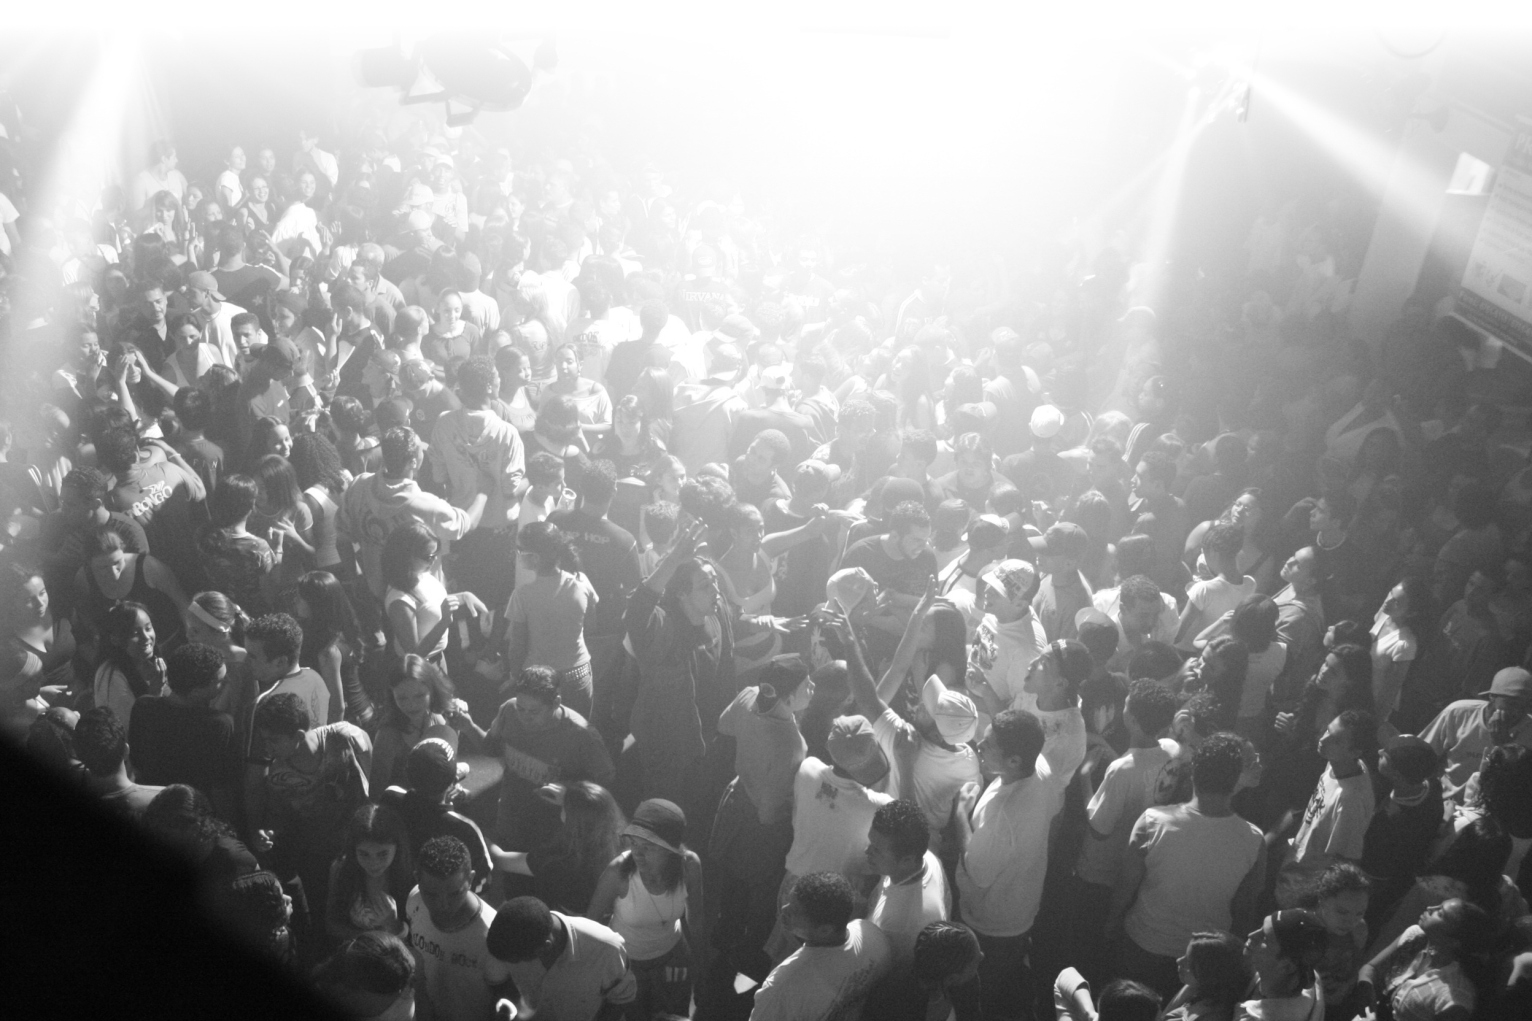
\includegraphics[scale=0.15,keepaspectratio=true]{img/imgs/7-diversao/-053.jpg}
\end{figure}

\begin{itemize}
\item  \textbf{Cooperativa Brasil:} Para quem gosta de um bom forró, sempre com
    shows diversos. A galera gosta muito da quarta-universitária. Maiores
    informações, acesse o site: \url{www.cooperativabrasil.com.br}.

\item  \textbf{Campinas Hall:} Muitas das festas mais legais da Unicamp
    acontecem lá (como a Festa Brega e a Festa do Contrário), perto da PUCC.
    É bem grande.

\item  \textbf{Delta Blues Bar:} O melhor do Blues \& Rock 'n Roll de Campinas
    \url{www.deltabluesbar.com.br}.

\item  \textbf{Barril da Máfia:} \url{www.barrildamafia.com.br}.

\item  \textbf{Swingers:} Tem bebidas caras e cada noite tem um tema, mas
    é melhor às quartas e quintas-feiras. Só homens maiores de 21 e mulheres com
    mais de 18 anos podem entrar.
    \url{www.grupohappynews.com.br/novo/swingers_campinas/index.php}

\item  \textbf{Golden:} Assim como a Swingers fica no Shopping D. Pedro. Balada
    cara, frequentada geralmente por gente mais velha.
    \url{www.goldstreetbar.com.br}

\item  \textbf{Camaleão Show:} Antigo Club Diesel. Primeira casa noturna de
    micareta e pagode de Campinas. \url{www.camaleaoshow.com.br}

\item  \textbf{Kraft:} Localizada próxima ao Taquaral (na Avenida Imperatriz
    Leopoldina), toca musica psi a noite toda e fica aberta até quase
    o amanhecer. Mulher entra de graça até a meia-noite.
    \url{www.clubekraft.com/}

\item  \textbf{Cambuí:} Neste bairro existem diversos barzinhos, a maioria
    é temático, alguns são um pouco caros e cobram covert. É um ótima escolha
    para quem tiver carro pois fica um pouco longe de Barão.

\end{itemize}

\subsection{Shopping Centers}

\begin{figure}[h!]
    \centering
    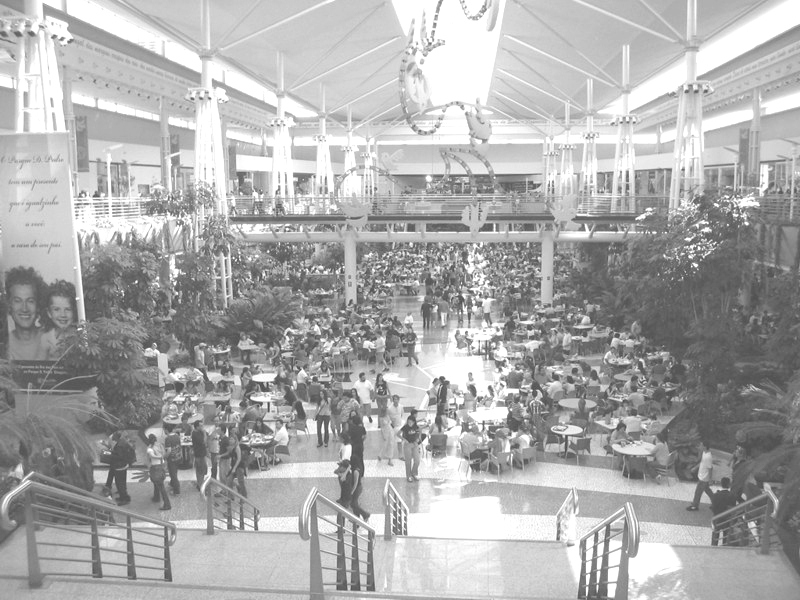
\includegraphics[scale=0.28,keepaspectratio=true]{img/imgs/7-diversao/-057.jpg}
\end{figure}

\begin{itemize}

\item  \textbf{Shopping Parque D. Pedro:} Foi considerado o maior shopping da
    América Latina até pouco tempo atrás. Localiza-se na Rodovia Dom Pedro, km
    137 (razoavelmente próximo a Unicamp). O ônibus 3.38 sai do terminal Barão
    vai para lá e para o Iguatemi. Página do shopping:
    \url{www.parquedpedro.com.br}.

\item  \textbf{Shopping Iguatemi:} Shopping normal, o mais antigo e o segundo
    maior de Campinas. Localiza-se na Avenida Iguatemi, 777. O 3.38 demora uns
    40 minutos para chegar lá. Frequentado por pela galera mais nova e pelo
    pessoal com um pouco mais de dinheiro. Página do shopping:
    \url{www.iguatemicampinas.com.br}.

\item  \textbf{Shopping Jaraguá:} Shopping pequeno e que possui duas unidades:
    Uma delas fica na Rua Conceiçao (Jaraguá Conceição); e a outra unidade fica
    na avenida Brasil (Jaraguá Brasil). Nesse segundo há duas salas de cinema
    que passam filmes "cult". O ônibus 3.30, no sentido terminal central --
    Unicamp para razoavelmente próximo ao Jaraguá Conceição, um ponto antes do
    ponto da prefeitura; e os ônibus 3.30, 3.31, 3.32 e 3.33 passam em frente ao
    Jaraguá Brasil.

\item  \textbf{Campinas Shopping:} Longe a dar com pau, mas as lojas não são
    muito caras. Localiza-se às margens das rodovias Anhanguera e Santos Dumont.
    Provavelmente você nunca irá lá. Página do shopping:
    \url{www.campinasshopping.com.br}.

\item  \textbf{Shopping Prado:} Shopping bem pequeno, as lojas não são muito
    caras, mas muito longe. Localiza-se na Avenida Washington Luís, 2480.
    Provavelmente você também nunca irá lá.

\item  \textbf{Galleria Shopping:} Muito bonito, mas lojas muito caras. Também
    localizado na Rodovia Dom Pedro, mas no km 131,5. O ônibus 3.00 sai do
    terminal de Barão Geraldo e passa lá. Página do shopping:
    \url{www.galleria.com.br}.

\item  \textbf{Shopping Unimart:} Shopping pequeno, as lojas não são muito
    caras. Localiza-se na Avenida John Boyd Dunlop, 350. O ônibus 1.34 sai do
    terminal de Barão Geraldo e passa próximo. Página do shopping:
    \url{www.unimart.com.br}.

\end{itemize}


%%%%% Transporte
% Não é preciso declarar nenhum cabeçalho

\section{Transporte}
\subsection{Voltar para casa}

Para os calouros de fora de Campinas, além de escolher a nova morada é
importante reunir informações sobre como realizar o trajeto entre sua cidade e
Campinas.

A forma usual é ir de ônibus, mas tenha em mente que a rodoviária é longe e os
trajetos de ônibus até lá são demorados. O endereço da rodoviária é: Rua Pereira
Lima, s/n. Há duas linhas que passam por lá: o 332 (que passa dentro da Unicamp)
para dentro da rodoviária, mas demora mais pra chegar que o 331, que sai do
terminal e para do lado de fora da rodoviária. Em horários de pico, o trajeto
pode demorar quase uma hora, então cuidado para não perder o horário do ônibus
para sua cidade. Também não se esqueça de portar algum cartão para andar nos
ônibus de Campinas, seja o Bilhete Único ou um dos dois cartões avulsos (Bilhete
1 Viagem e Bilhete 2 Viagens). Caso contrário, não será possível embarcar em um
ônibus.

Os que vêm de mais longe certamente farão uso do aeroporto de Viracopos, cujo
telefone é 3725-5000. Para chegar ao aeroporto existe a linha 193 que sai da
rodoviária e vai para o aeroporto, e também faz o trajeto de volta. Porém, ir
com ônibus circular pode ser um transtorno quando estiver com muita bagagem. Uma
outra alternativa é a Lirabus que também faz o traslado da rodoviária para o
aeroporto. A passagem da Lirabus custa R\$9,00 (R\$9,80 se sair da Rodoviária,
pois paga taxa de embarque) e os horários podem ser conferidos no site
\url{www.lirabus.com.br/}.

Para quem for usar os aeroportos da Grande São Paulo (Congonhas e Guarulhos),
existem os serviços de traslado, também oferecidos pela Lirabus. A tarifa para
Guarulhos sai R\$28,30 (R\$33,70 com taxa de embarque da Rodoviária), e para
Congonhas sai R\$24,45 (R\$29,90 com taxa de embarque da Rodoviária).

Para não pagar a taxa de embarque nos traslados da Lirabus, basta embarcar na
Sala VIP da Lirabus, localizada na Avenida Francisco Glicério, 435, em frente ao
Largo do Pará.

\subsubsection*{Caronas}

Uma forma barata e divertida de viajar, além de minimizar o tempo e dinheiro
gastos na viagem, é juntando alguns estudantes no mesmo carro e dividir as
despesas.
\begin{figure}[h!]  \centering
    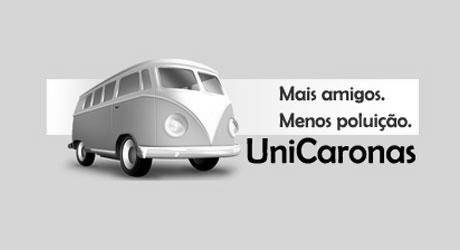
\includegraphics[width=.45\textwidth]{img/barao/unicaronas.jpg}
\end{figure}

O site UniCaronas (\url{unicaronas.com.br}) foi desenvolvido por dois
engenheiros de computação da Unicamp, com o intuito de facilitar o deslocamento
dos alunos entre cidades. Criado em 2007 como Caronas Unicamp e disponível
apenas para alunos da Unicamp, O site chegou a possuir mais de 20 mil usuários e
mediar caronas entre alunos de diversas universidades para várias cidades de
vários estados. Em 2014, o site se uniu ao Tripda (\url{tripda.com.br}),
aumentando imensamente a quantidade de destinos, mas mantendo as funcionalidades
básicas. No entanto, o site serve apenas para colocar os motoristas e caronistas
em contato, não assumindo responsabilidades sobre nenhuma das partes.

Recentemente foi criado o Mural de Caronas\\(\url{muraldecaronas.org}), que
igualmente ao UniCaronas exige um email institucional para realização do
cadastro no site. Entretanto, por enquanto só há opção de carona entre Barão
Geraldo e São Paulo. Além disso, há varios grupos de carona no Facebook, vale a
pena checá-los.

\subsection{Carro}

Para aqueles que tenham seu próprio veículo, é bom saber que a Unicamp tem
poucas vagas próximas aos locais de aulas. E o número de fiscais de trânsito tem
aumentado muito dentro do Campus.

\subsubsection*{Autoescolas}

Se você ainda não tem CNH e pretende obtê-la em Campinas, existem três opções de
autoescola em Barão Geraldo:

\begin{itemize}
    \item \textbf{Auto Escola Avenida} \\Endereço: Av. Albino J. B. De Oliveira,
658 \\Telefone: (19) 3288-0588

    \item \textbf{Auto Escola Advanced} \\Endereço: Av. Santa Isabel, 80
\\Telefone: (19) 3289-9499

    \item \textbf{CFC Brasil} \\Endereço: Av. Santa Isabel, 513
\\Telefone: (19) 3388-0513 / (19) 3289-2614
\end{itemize}

Porém recomendamos fortemente que você tire em sua cidade de origem se isso for
possível; os CFCs de Barão Geraldo são muito caros e muitas vezes você tem que
esperar meses para conseguir marcar aulas.

\subsubsection*{Recorrer de Multas}

Documentos:
\begin{itemize}
    \item Notificação e Fotocopia.
    \item CNH e Fotocopia.
    \item Documento do Carro e Fotocopia.
    \item Formulário:
      \url{bit.ly/1xW5E9z}.
    \item e anexos, se desejar.
\end{itemize}

E levá-los a:
\begin{itemize}
    \item \textbf{EMDEC} \\Horário: De segunda a sexta-feira, das 8h as 17h.
\\Endereço: Rua Dr. Salles Oliveira, 1028 -- Vila Industrial -- CEP 13035-270.
    \item \textbf{Poupatempo (Centro)} \\Horário: Das 8h às 18h, de segunda a
sexta-feira; e aos sábados, das 7h às 13h.  \\Endereço: Av. Francisco Glicério,
935.
    \item \textbf{Poupatempo (Campinas Shopping)} \\Horário: Das 9h às 19h, de
segunda a sexta-feira; e aos sábados, das 8h às 14h.  \\Endereço: Rua Jacy
Teixeira de Camargo, 940.
\end{itemize}

Fonte:
\url{bit.ly/1zntVk4}

\subsection{Ciclovias e ciclofaixas}

Campinas possui cerca de 27 quilômetros de ciclovias e de ciclofaixas. Algumas
dessas vias para bicicletas estão no distrito de Barão Geraldo. Uma delas é a
ciclovia que liga o campus da Unicamp a Av. Albino J. B. de Oliveira. A outra é
a ciclofaixa que liga a Av. Albino J. B. de Oliveira à moradia (Av. Santa
Isabel).

Nos domingos e feriados, das 7 até as 12 horas, as ciclofaixas ficam abertas
para os ciclistas.

\subsection{Ônibus}

Se não tem condução própria, ou carona, pode utilizar o transporte coletivo de
Campinas.

\begin{figure}[h!]  \centering
    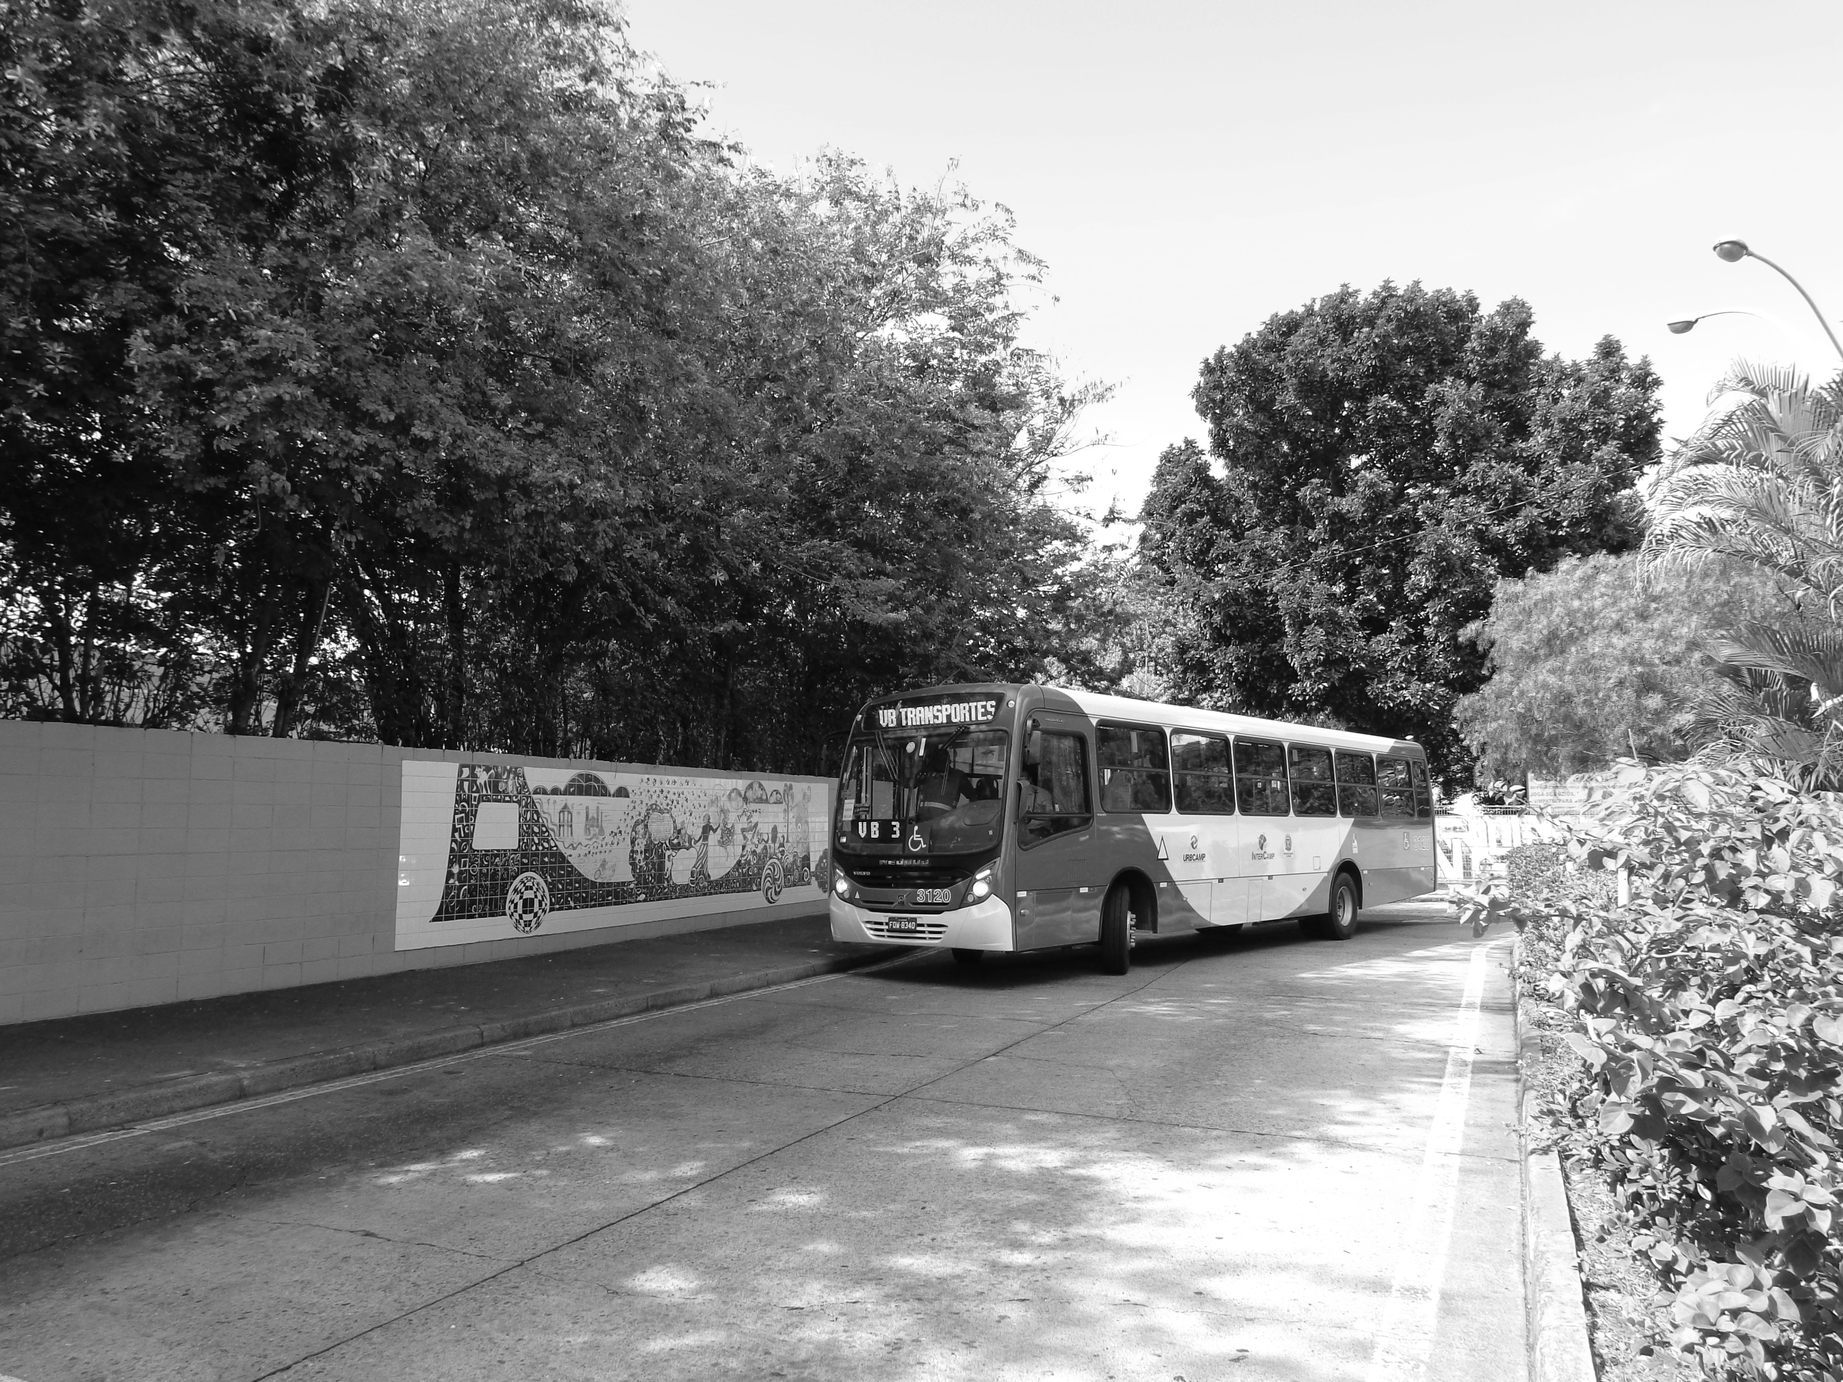
\includegraphics[width=.45\textwidth]{img/barao/onibus.jpg}
\end{figure}

O sistema de transporte público em Campinas é composto apenas por ônibus, e
chama-se InterCamp. O órgão municipal que organiza, gerencia e fiscaliza o
transporte público é a EMDEC (Empresa Municipal de Desenvolvimento de Campinas).
A bilhetagem eletrônica é organizada pela Transurc, a associação das empresas de
ônibus do transporte coletivo urbano de Campinas. Além das empresas, operam no
InterCamp cooperativas de transporte, originadas dos antigos perueiros.

Os ônibus em Campinas são identificados por um número de três dígitos, uma cor
(azul claro, azul escuro, vermelho ou verde), uma figura geométrica (círculo,
quadrado, triângulo ou tetragrama, para que os portadores de daltonismo possam
identificar os ônibus) e um nome.

A tarifa foi reajustada em junho de 2013 e custa R\$3,30. Apesar de existir
passe de estudante, universitários não tinham ao desconto, apenas estudantes de
ensino fundamental e médio. Em dezembro de 2014, o prefeito Jonas Donizete
sancionou lei que concede o desconto da passagem para estudantes universitários
de cursos presenciais.

Todo mês, em dois domingos, os usuários do transporte público de Campinas podem
usar os ônibus pagando metade da tarifa (o que dá R\$ 1,65). É o Passe Lazer. O
benefício vale apenas para os cartões avulsos e para o Bilhete Único Comum.

Existe quatorze linhas de ônibus que ligam o centro, alguns distritos, bairros e
terminais de Campinas ao distrito de Barão Geraldo. Algumas linhas desembarcam
os passageiros no terminal de Barão Geraldo, de onde seguem em outros ônibus
para a universidade. Já outras linhas vão direto para o campus. As trocas de
ônibus dentro do Terminal de Barão Geraldo são gratuitas, o que não ocorre em
outros terminais (no Terminal Mercado, por exemplo).

Em 2008 foi construída a nova e moderna rodoviária de Campinas, o terminal
multimodal Ramos de Azevedo. Além de transporte interestadual e municipal, o
espaço agrega um terminal metropolitano com o intuito de ligar as cidades da
Região Metropilitana de Campinas. Algumas linhas de ônibus internos de Campinas
também passam neste Terminal, como a linha 332.

Para consultar linhas de ônibus, há duas opções:
\begin{itemize}
  \item o sistema da EMDEC, que também possui um roteirizador bastante
interessante (\url{www.emdec.com.br/ABusInf/})
  \item o site Ônibus de Campinas, do Portal InterBuss, criado por entusiastas
de ônibus, dentre eles, um veterano da Computação
(\url{www.portalinterbuss.com.br/campinas/})\ldots
\end{itemize}

Outra ferramenta interessante para quem pretende usar o transporte público em
Campinas é o aplicativo Moovit, disponível para iOS, Android e Windows
Phone. Com ele, é possível visualizar os pontos de ônibus ao seu redor e as
linhas que passam neles. Além disso, também funciona como roteirizador,
indicando as linhas que você pode pegar para chegar a um lugar da cidade.

Para reclamações do transporte público, é necessário utilizar o canal 156 da
Prefeitura de Campinas. Ele pode ser acessado através do telefone 156, através
do site da Prefeitura (\url{www.campinas.sp.gov.br/servico-ao-cidadao/156.php}),
e através do aplicativo 156 Mobile Campinas, disponível para Android. As
reclamações são respondidas pelos órgãos de fiscalização da EMDEC, e todo o
processo pode levar até seis meses. Entretanto, é o único meio que pode resultar
em ações efetivas, como multas e advertências. Além disso, a reclamação entra
nas estatísticas da EMDEC, que são utilizadas para direcionar agentes de
fiscalização e, caso haja algum problema operacional de itinerário ou de
horário, também podem ser feitas alterações para otimização do serviço.

\subsubsection*{Bilhete Único}

O Bilhete Único foi implantado com o objetivo de facilitar o transporte daqueles
que se utilizam de ônibus. No prazo de 2 horas, o usuário pode usar até três
ônibus pagando apenas uma passagem. Além disso, agora o usuário tem dois
créditos negativos para utilizar caso o saldo seja zerado. O cadastro é rápido e
o cartão sai na hora.

O Bilhete Único Comum pode ser feito nos seguintes locais:
\begin{itemize}
  \item sede da Transurc, na Rua Onze de Agosto, 757
  \item nos terminais de ônibus (guichês da Transurc, sempre próximos à entrada)
  \item na Loja do Bilhete Único, na Av. Anchieta, 55
  \item no posto da Transurc do Poupatempo Centro (Av. Francisco Glicério, 935,
térreo)
  \item na Drogaria Sidarta do Balão do Londres (Av. John Boyd Dunlop) \ldots
\end{itemize}

Para a primeira recarga, exige-se o pagamento de uma tarifa (o que atualmente
fica em R\$ 3,30).

Para recarregar o cartão, além dos terminais, também tem diversos
estabelecimentos comerciais credenciados a fazer a recarga do cartão, que podem
ser vistos na página:
\url{bit.ly/13Aav2C}.

\subsubsection*{Como embarcar sem Bilhete Único}

Campinas vem extinguindo a função do cobrador, substituindo-o pela bilhetagem
eletrônica. Várias linhas já rodam sem cobrador, e provavelmente muitos lerão
este texto quando já estiverem completamente extintos do sistema.

A partir de 1º de fevereiro de 2015, o pagamento não poderá mais ser feito em
dinheiro dentro dos ônibus. Com isso, os usuários deverão entrar nos veículos
portando o Bilhete Único (vide sub-seção acima para mais informações) ou um
cartão avulso, chamado Bilhete Viagem.

São dois Bilhetes Viagem: o Bilhete 1 Viagem e o Bilhete 2 Viagens.

O Bilhete 1 Viagem é adquirido pelo valor de R\$ 5,30, e pode ser usado apenas
uma vez, pois não dá direito a integração. Também não pode ser recarregado.  Por
isso, é ideal apenas para quem for utilizar ônibus uma única vez.

O Bilhete 2 Viagens é adquirido pelo valor de R\$ 8,60, pode ser usado por duas
vezes, e depois ainda pode ser recarregado em qualquer posto de recarga do
Bilhete Único. É o cartão ideal para quem pretende utilizar ônibus mais de uma
vez, mas não pretende fazer o Bilhete Único.

Os R\$ 2,00 acima da tarifa vigente pagos na aquisição de ambos os Bilhetes
Viagem se referem ao custo de casco do cartão, que são devolvidos ao usuário se
ele entregar o cartão vazio em um dos postos da Transurc (sede da Transurc,
terminais, Loja do Bilhete Único ou posto da Transurc do Poupatempo Centro).

Ambos os Bilhetes Viagem podem ser adquiridos nos postos da Transurc ou na rede
credenciada
(\url{bit.ly/13Aav2C}).


%%%%% Outras necessidades
% Este arquivo .tex será incluído no arquivo .tex principal. Não é preciso
% declarar nenhum cabeçalho

\section{Outras necessidades}
\subsection{Supermercados}

No centro de Barão há três supermercados: o Pague Menos (antigo Super Barão ou
Super Ladrão) o Pão-de-Açúcar e o Dalben. Ambos Pague Menos e Pão-de-Açúcar são
muito caros, mas o Page menos tem boas promoções de segunda e terça-feiras. Cada
um é melhor/mais barato para alguma coisa. Só indo bastante em cada um é que
você pega o jeito.

\begin{figure}[h!]
    \centering
    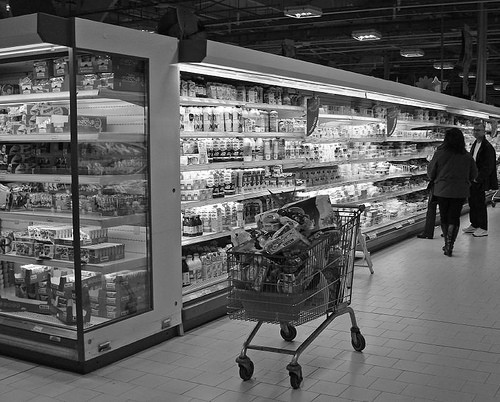
\includegraphics[scale=0.42,keepaspectratio=true]{img/imgs/9-outras_necessidades/supermercado.jpg}
\end{figure}

O Dalben é maior e geralmente tem coisas mais baratas que o Pão-de-Açúcar. Às
segundas e terças (no Dalben e no Pague Menos) e às terças (no Pão de Açúcar) há
preço promocional de frutas e verduras. O Dalben localiza-se no alto da Avenida
1, na entrada de Barão Geraldo. O Barão funciona de segunda a sábado das 7h às
22h e domingos das 8h às 20h e o Pão de Açúcar funciona de domingo
a quinta-feiradas 7h às 23h, sextas e sábados das 7h às 24h. Na moradia, há
outro Pague Menos e o Benatti, e no Real Parque outra loja do Pague Menos.

Há também lojas de conveniência (como as AM/PM em frente à Unicamp na Av. 1,
e no Rio das Pedras e a da Shell no fim da avenida 2 e em frente ao terminal,
a mais barata das 4) que embora mais caras que os supermercados, podem funcionar
em horários que esses não ou serem mais perto de onde você mora.

Em frente ao terminal Barão há o Recanto Bela Fruta, que não é exatamente um
supermercado, mas é o melhor lugar de Barão para comprar frutas, verduras
e legumes. Vende também algumas coisas de supermercado como pão, leite, iogurte,
mupy etc. Neste mesmo esquema funciona o varejão Oba, que fica na avenida Santa
Isabel, perto da pizzaria Sapore. Na estrada da Rhodia, depois da Padaria Di
Capri, há a frutaria Rio das Pedras, que tem preços no nível do Pão de Açúcar
e do Pague Menos, mas é mais próximo pra quem vive na Cidade Universitária 2,
por exemplo.

Se você tiver carro, ou conhecer alguém que tenha, junte um pessoal e faça suas
compras no Tenda Atacado ou no Atacadão. Os dois são muito mais baratos que
qualquer supermercado e têm muita variedade. Ah, e nem tudo é atacado, vende
umas coisas a varejo lá também. Para chegar aos dois, saindo de Barão pelo
Tapetão, pegue a D. Pedro sentido Anhanguera. Assim que você entrar na D. Pedro,
você já vai enxergar o Atacadão, à direita. Para ir ao Tenda siga mais um pouco
na D.  Pedro e saia logo depois do CEASA à direita.

Outras opções para quem tem carro são: O Carrefour, localizado na Rodovia D.
Pedro e o Wal-Mart, que fica no Shopping Parque D. Pedro.

\subsection{Utilidades em geral}

\begin{itemize}
\item  \textbf{Ki-Água}
\begin{itemize}
\item  Telefone: (19) 3289-4659
\item  Endereço: Rua Eduardo Modesto, 240
\end{itemize}

\item  \textbf{Circuito das Águas}
\begin{itemize}
\item  Telefone: (19) 3289-4930
\item  Endereço: Rua Júlia Leite de Barros, 182
\end{itemize}

\item  \textbf{Água Mineral Serrana}
\begin{itemize}
\item  Telefone: (19) 3289-4602
\item  Endereço: Rua Albino José Barbosa de Oliveira, 658
\end{itemize}

\item  \textbf{Real Gás}
\begin{itemize}
\item  Telefone: (19) 3289-1786
\item  Endereço: Rua Eduardo Pereira de Almeida, 570
\end{itemize}

\item  \textbf{Genebra Gás}
\begin{itemize}
\item  Telefone: (19) 3289-3622
\item  Endereço: Avenida Santa Isabel
\end{itemize}

\item  \textbf{Drogaria Vitória}
\begin{itemize}
\item  Telefone: (19) 3289-9926
\item  Endereço: Avenida Ruberley Bueretto da Silva, 1015
\end{itemize}

\item  \textbf{Drogaria Nova Barão}
\begin{itemize}
\item  Telefone: (19) 3289-6191
\end{itemize}

\item  \textbf{Rede Farmaxima}
\begin{itemize}
\item  Telefone: (19) 3289-2824 / (19)3289-4054
\item  Endereço: Avenida Dr. Romeu Tórtima, 255
\end{itemize}

\item  \textbf{Drogaria Sidarta}
\begin{itemize}
\item  Telefone: (19) 3289-1999
\item  Endereço: Avenida Prof. Atílio Martini, 190
\end{itemize}

\item  \textbf{New Laundry Lavanderia}
\begin{itemize}
\item  Telefone: (19) 3289-3922
\item  Endereço: Rua Francisca Resende Merciai, 54
\end{itemize}

\item  \textbf{Desentupimento 24 horas}
\begin{itemize}
\item  Telefone: (19) 3242-1249
\end{itemize}

\item  \textbf{Carpintaria São Jorge de Barão}
\begin{itemize}
\item  Telefone: (19) 3289-3399
\item  Endereço: Avenida Santa Isabel, 1882
\end{itemize}

\item  \textbf{CPFL (companhia de luz)}
\begin{itemize}
\item  Telefone: 0800-010-1010
\end{itemize}

\item  \textbf{Sanasa (companhia de água)}
\begin{itemize}
\item  Telefone: 0800-772-1195
\end{itemize}

\item  \textbf{Luigi Cabelereiro}
\begin{itemize}
\item  Telefone: (19) 3288-0198
\end{itemize}

\item  \textbf{João Cabelereiros}
\begin{itemize}
\item  Telefone: (19) 3289-3084
\item  Endereço: Rua Orácio Leonardi, 92
\end{itemize}

\item  \textbf{Armazém da Foto}
\begin{itemize}
\item  Telefone: (19) 3289-0975
\end{itemize}

\item  \textbf{Empresa de Correios e Telégrafos (Correios)}
\begin{itemize}
\item  Endereço 1: Avenida Santa Isabel, 218 -- Centro de Barão.
\item  Telefone 1: (19) 3288-0244.
\item  Endereço 2: Rua Carlos Gomes, 241 -- Campus da Unicamp (próximo ao
       ginásio e Instituto de Artes).
\item  Telefone 2: (19) 3289-7288 e (19) 3521-7642.
\end{itemize}
\end{itemize}

\subsection{Bancos}

\begin{figure}[h!]
    \centering
    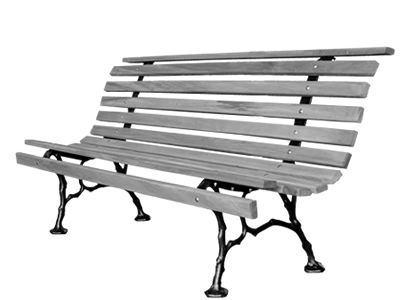
\includegraphics[scale=2.28,keepaspectratio=true]{img/imgs/9-outras_necessidades/raizmadeira.png}
\end{figure}

\begin{itemize}
    \item  \textbf{Banco do Brasil:} Com a compra da Nossa Caixa pelo BB, há
    3 agências: Uma localizada perto da Reitoria, outra no centro de Barão,
    perto do Santander, e outra no centro de Barão perto do Pague Menos. Há
    caixa eletrônico onde antigamente era a agência do BB perto dos Correios.

    \item  \textbf{Bradesco:} Agência no centro de Barão, do lado do Banco do
    Brasil e em frente do Santander. Próxima ao Terminal Barão.

    \item  \textbf{Caixa Econômica Federal:} Localizada na frente do Pão de
    Açúcar.
    
    \item  \textbf{Citibank:} Localizado no alto da avenida 2, próximo ao posto
    Shell.

    \item  \textbf{Itaú:} Possui uma agência na Unicamp, próximo à Reitoria
    e à agência do Santander, e outra na avenida Santa Isabel, do lado da
    sorveteria. Existe também o Itaú Personnalité, próximo ao Pão de Açuar e ao
    McDonalds.

    \item  \textbf{Santander:} Há quatro agêncais em Barão: duas localizadas ao
    lado da Reitoria, outra na praça do Ciclo Básico e a outra próxima ao
    Terminal Barão.
\end{itemize}

\subsection{Sebos e livrarias}

Em Barão há três sebos: O Curupira, o Cronópio e o Galpão. Geralmente você não
encontra muita coisa boa de computação neles, mas não custa procurar. O Curupira
fica na rua do Terminal, bem em frente a ele. Não é difícil achar. O Galpão fica
perto do Terminal. Saindo do terminal pela avenida marginal à Albino de
Oliveira, vire a primeira à esquerda e a segunda à direita. Funciona de segunda
à sexta até às 18h. O Cronópio fica na mesma rua do Galpão, só que bem longe,
próximo à padaria Fiori. Seguindo a Santa Isabel, vindo do Centro de Barão, vire
à esquerda na esquina que tem uma pizzaria (antes da Fiori). Vire na primeira
à esquerda e você está no Cronópio (Lá também é um restaurante barato
e gostoso).

Na Unicamp há a livraria Toledo, que fica na Faculdade de Educação (Pedago), tem
pouca coisa de Computação lá mas alguma coisa de Matemática. Também há
a livraria da Unicamp (no IEL), tem preços bons mas não tem quase nada de
Exatas. Já a Livraria da Química tem livros de exatas, e geralmente eles
conseguem importar a um preço bom. Outras livrarias são a Fnac (no Shopping D.
Pedro), a Saraiva e a Cultura (no Shopping Iguatemi) e a Siciliano (no Shopping
Galeria).

Mais uma dica: Antes de comprar um livro, veja se você vai usar muito ele, se
não tem bastante na biblioteca, se algum veterano legal não pode te emprestar ou
te vender, ou se não rola tirar xerox. Você compra livro só se você precisar
e/ou quiser muito. Caso vá comprar, atente para livrarias virtuais, que podem
ter preços muito menores (pesquise sempre no Buscapé
(\url{www.buscape.com.br})) e emitem boletos para você pagar no banco.
Em alguns casos, a livraria da Editora (localizada no piso térreo da BC) pode
trazê-lo por um preço menor ainda -- consulte sempre!

Uma última dica: Não compre o livro de G.A. (MA141). Estude pelo Stewart II
(livro de Cálculo II), pelo Steinbruch ou pelo livro do Paulo
Boulos. Os três são muito melhores que ele. Se você quiser os exercícios para
estudar para os testes pegue na internet ou tire xerox. Use os outros livros
para estudar.

\begin{figure}[h!]
    \centering
    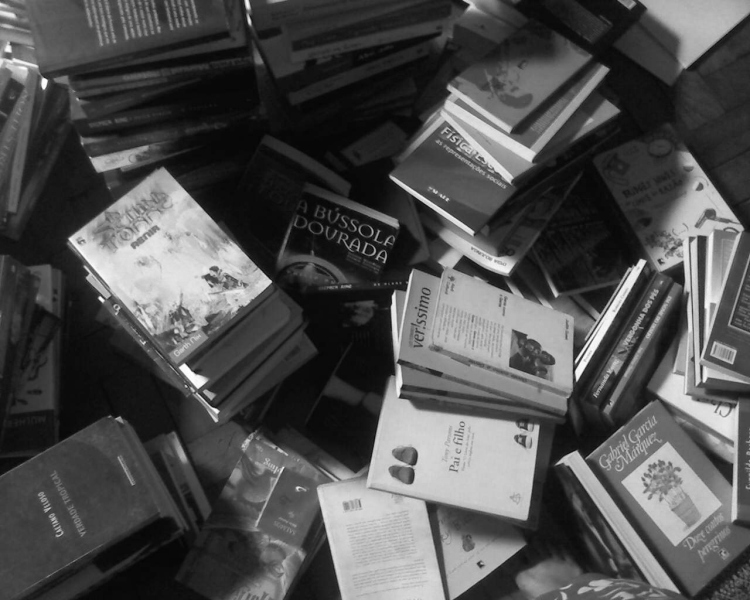
\includegraphics[scale=0.29, keepaspectratio=true]{./img/imgs/9-outras_necessidades/-068.jpg}
\end{figure}


\begin{itemize}
\item  \textbf{Sebo Curupira}
\begin{itemize}
\item  Endereço: Avenida Albino José B. de Oliveira, 980
\item  Telefone: (19) 3289-7522
\end{itemize}

\item  \textbf{Sebo Galpão}
\begin{itemize}
\item  Endereço: Rua Francisco Barros Filho, 16
\item  Telefone: (19) 3289-2044
\end{itemize}

\item  \textbf{Sebo Valise de Cronópio}
\begin{itemize}
\item  Endereço: Rua Francisco de Barros Filho, 426
\item  Telefone: (19) 3289-0028
\end{itemize}
\end{itemize}

\subsection{Bicicletarias}

\begin{itemize}
\item  \textbf{Bicicletaria Barão}
\begin{itemize}
\item  Endereço: Avenida Santa Isabel, 446.
\item  Telefone: (19) 3249-0449.
\end{itemize}

\item  \textbf{Rei do Pedal}
\begin{itemize}
\item  Endereço: Avenida Santa Isabel, 74.
\item  Fone: (19) 3289-9258.
\end{itemize}

\item  \textbf{Via Bike}
\begin{itemize}
\item  Endereço: Avenida Albino José Barbosa de Oliveira, 1074.
\item  Telefone: (19) 3289-9888.
\end{itemize}
\end{itemize}

\subsection{Escolas de idiomas}

\begin{itemize}
\item  \textbf{CCAA}
\begin{itemize}
\item  Endereço: Rua Professor Luciano Venere Decourt, 290.
\item  Telefone: (19) 3249-0202.
\item  E-mail: barao [@] ccaa [.] com [.] br
\item  Site: \url{www.ccaa.com.brbarao}
\end{itemize}

\item  \textbf{CCBEUC -- Centro Cultural Brasil Estados Unidos -- Campinas}
\begin{itemize}
\item  Endereço: Avenida Romeu Tórtima, 531.
\item  Telefone: (19) 3249-0275.
\item  E-mail: admbg [@] ccbeuc [.] com [.] br
\item  Site: \url{www.ccbeuc.com.br}
\end{itemize}

\item  \textbf{CNA}
\begin{itemize}
\item  Endereço: Avenida Dr. Romeu Tortima, 553.
\item  Telefone: (19) 3289-4700.
\item  Fax: (19) 3289-4700.
\item  E-mail: baraogeraldo [@] cna [.] com [.] br
\item  Site: \url{www.cna.com.brbaraogeraldo}
\end{itemize}

\item  \textbf{HAVAD}
\begin{itemize}
\item  Endereço: Avenida Romeu Tórtima, 522.
\item  Telefone: (19) 3288-0012.
\item  Fax: (19) 3249-0488.
\item  Email: havad [@] havad [.] com [.] br
\item  Site: \url{www.havad.com.br}
\end{itemize}

\item  \textbf{In Touch}
\begin{itemize}
\item  Endereço: Rua Antônio Augusto de Almeida, 517 -- Cidade Universitária.
\item  Telefone: (19) 3289-3481.
\item  E-mail: secretaria [@] intouch [.] art [.] br
\item  Site: \url{www.intouch.art.br}
\end{itemize}

\item  \textbf{INOVA -- Escola de Inglês}
\begin{itemize}
\item  Endereço: Avenida Romeu Tórtima, 391.
\item  Telefone: (19) 3288-0071.
\item  E-mail: fale [@] inovalinguas [.] com [.] br
\item  Site: \url{www.inovalinguas.com.br}
\end{itemize}

\item  \textbf{Real Time}
\begin{itemize}
\item  Endereço: Rua Agostinho Páttaro, 47 (esquina com a do praça do coco).
\item  Telefone: (19) 3289-6240.
\item  E-mail: barao [@] rtidiomas [.] com [.] br
\item  Site: \url{www.realtimeenglish.com.br}
\end{itemize}

\item  \textbf{Wizard}
\begin{itemize}
\item  Endereço: Rua João Batista Antonioli, 90.
\item  Telefone: (19) 3289-6199.
\end{itemize}

\item  \textbf{Yazigi}
\begin{itemize}
\item  Endereço: Avenida Dr. Romeu Tórtima, 500.
\item  Telefone: (19) 3249-2375.
\item  Site: \url{www.yazigi.com.br}
\end{itemize}
\end{itemize}

\subsection{Igrejas}

\begin{itemize}
\item  \textbf{IBCU -- Igreja Batista da Cidade Universitária}
\begin{itemize}
\item  Endereço: Rua Tenente Alberto Mendes Jr., 5.
\item  Telefone: (19) 3289-4501.
\item  Site: \url{www.ibcu.org.br}
\item  E-mail: jovens [@] ibcu [.] org [.] br
\end{itemize}

\item  \textbf{IBBG -- Igreja Batista de Barão Geraldo}
\begin{itemize}
\item  Endereço: Rua Luiz Vicentim, 284.
\item  Telefone: (19) 3289-1793.
\end{itemize}

\item  \textbf{IPBG -- Igreja Presbiteriana de Barão Geraldo}
\begin{itemize}
\item  Endereço: Rua Francisco Andreo Aledo, 141 (próximo à praça do coco e moradia).
\item  Telefone: (19) 3289-3239.
\end{itemize}

\item  \textbf{Igreja do Nazareno Betânia}
\begin{itemize}
\item  Endereço: Rua Manoel Antunes Novo, 98.
\item  Telefone: (19) 3289-7379.
\end{itemize}

\item  \textbf{Assembleia de Deus -- Ministério de Belém}
\begin{itemize}
\item  Endereço: Rua Júlia Leite de Barros, 54 (próximo à moradia da Unicamp).
\item  Telefone: (19) 3249-0035.
\item  Site: \url{www.adbarao.com.br}
\end{itemize}

\item  \textbf{Paróquia Santa Isabel}
\begin{itemize}
\item  Endereço: Rua Benedito Alves Aranha, 226.
\item  Telefones: (19) 3289-1101 e (19) 3289-2323
\item  Site: \url{www.paroquiasantaisabel.org.br}
\end{itemize}

\item  \textbf{Comunidade do Estudante Universitário}
\begin{itemize}
\item  Endereço: Rua Dr. Ruberlei Boaretto da Silva, 785.
\item  E-mail: ceu.campinas@gmail.com
\end{itemize}
\end{itemize}

\subsection{Postos de combustível}

\begin{itemize}
\item  \textbf{Auto Posto Campineira}
\begin{itemize}
\item  Endereço: Avenida Albino Jose Barbosa de Oliveira, 1480.
\item  Telefone: (19) 3289-5991.
\end{itemize}

\item  \textbf{Auto Posto Barbieri de Barão Geraldo}
\begin{itemize}
\item  Endereço: Avenida Albino Jose Barbosa de Oliveira, 1001 (próximo ao terminal).
\item  Telefone: (19) 3289-1917 e (19) 9768-6713.
\end{itemize}

\item  \textbf{Centro Automotivo Cidade Universitária LTDA}
\begin{itemize}
\item  Endereço: Avenida Doutor Romeu Tortima, 1541.
\item  Telefones: (19) 3289-8457, (19) 3289-9934 e (19) 3289-9199.
\end{itemize}

\item  \textbf{Transo Combustíveis LTDA}
\begin{itemize}
\item  Endereço: Avenida Santa Izabel, 1030 (próximo à moradia).
\item  Telefone: (19) 3289-1012.
\end{itemize}

\item  \textbf{Esso Auto Posto Futuro}
\begin{itemize}
\item  Endereço: Avenida Albino Jose Barbosa Oliveira, 360 (logo na entrada do distrito de Barão).
\item  Telefone: (19) 3289-4332.
\end{itemize}

\item  \textbf{Posto Vô João}
\begin{itemize}
\item  Endereço: Avenida Albino José Barbosa de Oliveira, 2151.
\item  Telefones: (19) 3289-3388 e (19) 3289-6594.
\item  Site: \url{www.vojoao.com/}
\end{itemize}
\end{itemize}

OBS: Dentro do campus há um posto de combustível (próximo à descida da FEAGRI),
mas atende apenas veículos oficiais.

\twocolumn
\section{SIGLAS malucas}

Nesta sessão serão dadas algumas explicações sobre algumas siglas, códigos
e outros termos muito usados dentro da Unicamp. Aí vão eles:

\begin{itemize}
    \item  \textbf{CCG (Comissão Central de Graduação):} Órgão colegiado da
    Unicamp, é encarregada da orientação, supervisão e revisão periódica do
    ensino na Universidade. Cabe recurso à CCG de quaisquer decisões das
    Unidades afetando o ensino.

    \item  \textbf{CCPG (Comissão Central de Pós-Graduação):} Órgão colegiado da
    Unicamp, é encarregada da orientação, supervisão e revisão periódica da
    pós-graduação na Universidade. Cabe recurso à CCPG de quaisquer decisões das
    Unidades afetando o ensino.

    \item  \textbf{Consu (Conselho Universitário):} O Consu é o órgão máximo da
    Universidade, acima do reitor, embora o ele faça parte e influencie
    fortemente suas decisões.  Existe representação discente no Consu, eleita
    juntamente com a Coordenadoria do DCE.

    \item  \textbf{Congregação:} É o órgão colegiado do Instituto ou Faculdade.
    Cabe recurso à Congregação da Unidade de Ensino de quaisquer decisões dos
    Departamentos e das Coordenações de Curso.

    \item  \textbf{Departamento:} É administrado por um professor-chefe e um
    Conselho Departamental, é a menor unidade administrativa, didática
    e científica da Universidade, sendo responsável pelo desenvolvimento dos
    programas de ensino, pesquisa e extensão dos serviços à comunidade. Todo
    instituto e faculdade da universidade possui o seu conjunto de
    departamentos, conhecidos através de siglas.

    \item  \textbf{CI (Conselho Interedepartamental):} Este é um "braço" da
    congregação, responsável por tratar de assuntos menores, como despesas
    e atribuições de sala. Fazem parte deste órgão, além de um representante
    discente, o diretor do instituto, os coordenadores e os chefes de
    departamentos.

    \item  \textbf{CDI (Comissão Diretora de Informática):} Outro braço da
    congregação, responsável por tratar de assuntos relacionados aos ambientes
    computacionais, deliberando sobre a atualização de infraestrutura,
    a organização da rede, endereços de internet e similares.

    \item  \textbf{CG (Coordenadoria/Comissão de Graduação):} É o órgão da
    unidade responsável pelos seus cursos de graduação. Sempre que houver algum
    problema ou deficiência no curso, é este órgão que vocês devem procurar.
    Cada curso tem um coordenador (que faz parte da CG), sendo que, atualmente,
    o professor Hélio Pedrini é o coordenador da Ciência e os professores
    Eduardo Xavier (IC) e o Akebo Yamakami (FEEC) são os coordenadores da
    Engenharia.

    \item  \textbf{CPG (Coordenadoria/Comissão de Pós-Graduação):} Este
    é o órgão responsável pela pós-graduação no Instituto, coordenando as
    disciplinas oferecidas e as matrículas na pós. O coordenador atual
    é o professor Paulo Lício de Geus. Os alunos tem direito a voz e voto nos
    colegiados (instâncias decisórias compostas por várias pessoas) da Unicamp,
    tendo representação discente em número correspondente a um quinto (1/5) dos
    membros. Geralmente, os representantes discentes são eleitos pelos
    estudantes ou indicados pelos centros acadêmicos. O exercício da
    representação estudantil e atividades decorrentes não exonera o aluno da
    frequência nas atividades escolares, com exceção da participação em reuniões
    em órgãos colegiados, nos horários em que estes se reúnem para deliberar.

    \item  \textbf{DCE (Diretório Central de Estudantes):} É a entidade de
    representação dos estudantes de graduação da Unicamp, competindo-lhe ainda
    designar representantes estudantis para os órgãos colegiados da
    Universidade.

    \item  \textbf{DAC (Diretoria Acadêmica):} É o órgão executivo
    e informativo, incumbido do registro e controle das atividades discentes da
    Unicamp. Cuida das matrículas, alteração de matrícula, emissão de documentos
    e relatórios, como o histórico escolar, realiza reserva de salas, entre
    outras atividades.

    \begin{figure*}[hb!]
        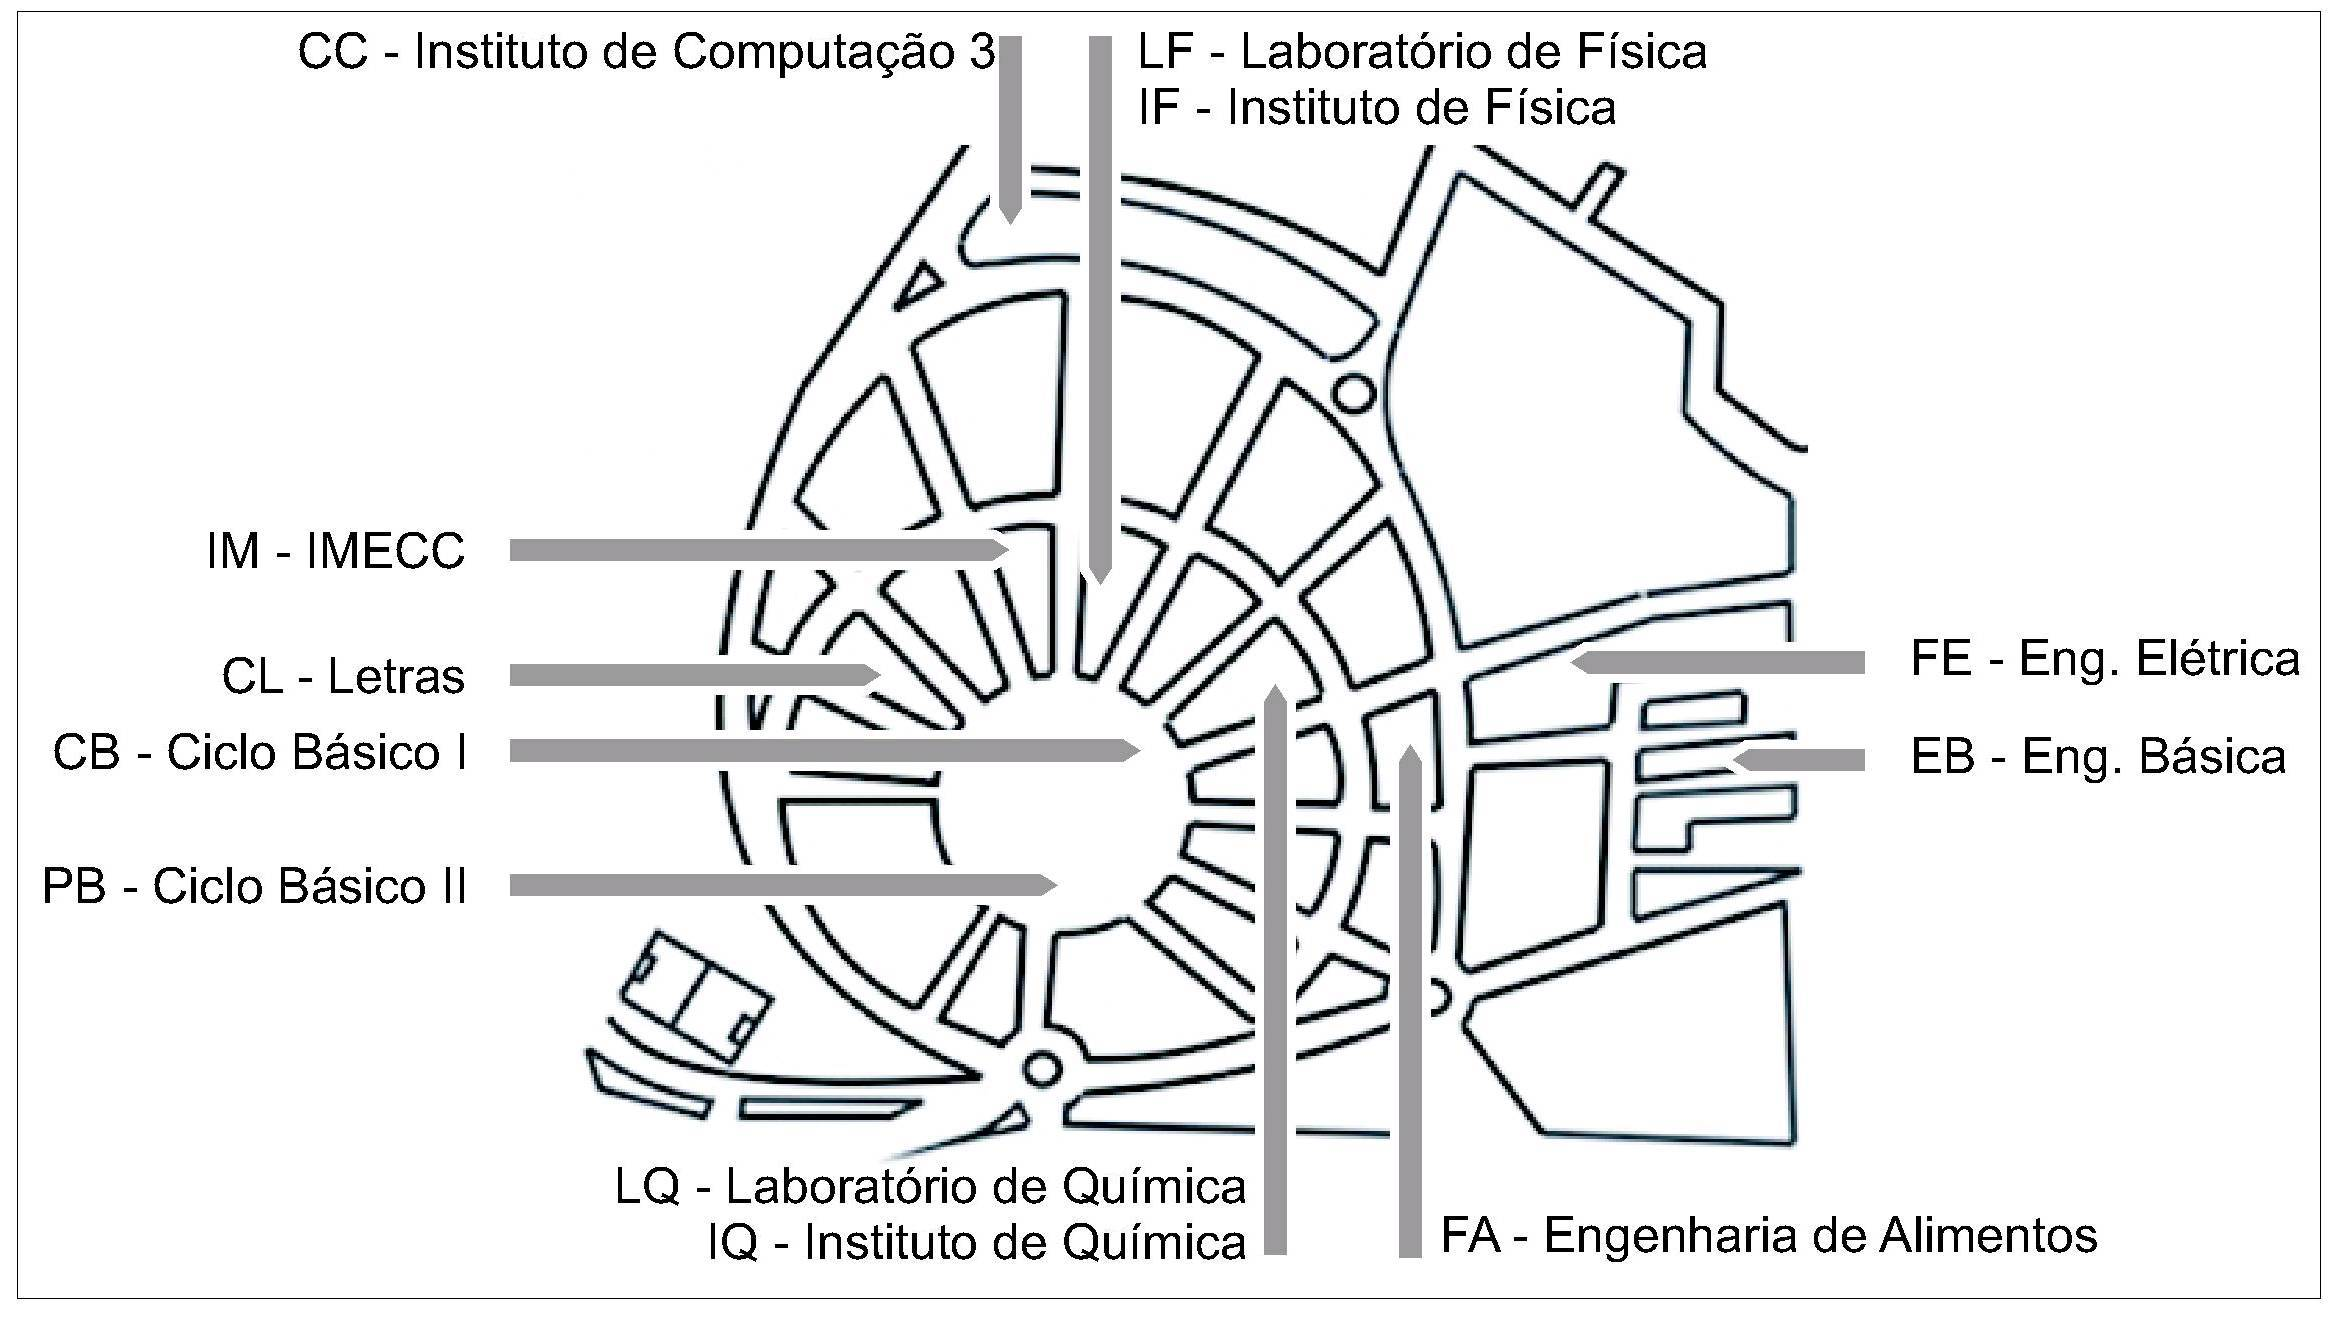
\includegraphics[scale=0.26, keepaspectratio=true]{img/imgs/10-siglas_malucas/mapa_siglas.jpg}
        \caption{Mapa com as siglas da sala de aula}
        \label{fig:mapa_siglas}
    \end{figure*}

    \item  \textbf{SAE (Serviço de Apoio ao Estudante):} É encarregado da
    execução de programas de assistência desenvolvidas pela Universidade, por
    iniciativa própria ou mediante convênios firmados com entidades
    especializadas.

    \item  \textbf{Crédito:} Unidade elementar de horas-aula de qualquer curso
    da Unicamp. Um crédito equivale a uma hora-aula semanal, ou a 15 horas-aula
    semestrais.

    \item  \textbf{Período letivo:} É um nome complicado para se referir ao
    semestre.

    \item  \textbf{Currículo pleno:} É o conjunto de disciplinas do curso que
    o aluno tem que cursar.

    \item  \textbf{CR (Coeficiente de Rendimento):} Valor entre 0 e 1 que
    é a média ponderada das notas obtidas em todas as disciplinas até o momento.
    É calculada usando como pesos o número de créditos de cada disciplina.

    \item  \textbf{CP (Coeficiente de Progressão):} É a porcentagem do curso que
    você já cumpriu. Por exemplo, se você tem CP = 0,6123 significa que você
    cumpriu 61,23\% do curso. Você se forma quando o seu CP for 1 (100\% do
    curso completo). É importante saber o CP quando for fazer algum estágio, ou
    um TCC (Trabalho de Conclusão de Curso), ou quando for cursar disciplinas
    que tenham como pré-requisito AA4xy.

    \item   \begin{itemize}
            \item  \textbf{CPF (Coeficiente de Progressão Futuro):} Além do CP,
            também tem o CPF, que além do nome de um documento é o CP que você
            terá no fim do semestre caso passe em todas as disciplinas.
            \item  \textbf{CPE (Coeficiente de Progressão Exigido):} Além do CP
            e do CPF há o CPE. O CPE foi instituído a partir de 2005 e é usado
            para fins de cancelamento, ou não, de matrícula. Para que o aluno
            possa continuar a fazer o curso, ele precisa ter um CP maior ou
            igual ao CPE daquele semestre. Tanto o CP, como o CPE e o CPF
            existem somente nos cursos de graduação.
            \end{itemize}

    \item  \textbf{Pré-requisito:} Matéria(s) que precisa(m) ter sido cursada(s)
    para que se possa fazer outra(s) matéria(s). Existem dois tipos de
    pré-requisitos: Os pré-requsitos totais, mais comuns, do qual é exigido
    tanto a aprovação por nota como por frequência e os pré-requisitos parciais,
    mais raros, do qual o aluno não precisa ter sido aprovado por nota, mas tem
    que ter tido aprovação por frequência e nota final maior ou igual a 3,0. Os
    pré-requisitos parciais são identificados com um asterisco na frente do
    código da disciplina (não confundir com um apontador).

    \item  \textbf{AA4xy:} Um tipo de pré-requisito. Não se trata de nenhuma
    disciplina. Para fazer disciplinas com esse pré-requisito, o aluno tem que
    tem um CP maior ou igual a 0,xy.

    \item  \textbf{AA200:} Outro tipo de pré-requisito existente, mais presente
    em disciplinas eletivas. Também não se trata de nenhuma disciplina. É apenas
    uma autorização da coordenadoria do curso. Se sobrar vagas para a disciplina
    e a coordenadoria do curso for com a sua cara você faz a disciplina.

    \item  \textbf{PB (Prédio Básico)} Também conhecido como Ciclo Básico II,
    é um prédio com várias salas de aula, que fica em frente ao Bandejão,
    e serve várias unidades que não possuem espaço físico suficiente para
    comportar seus alunos. No segundo andar ficam as salas de aula (PB01 a PB12)
    e no terceiro andar ficam os auditórios (PB13 a PB18).

    \item  \textbf{CB (Ciclo Básico I):} Tem finalidade idêntica ao PB, só que
    é muito melhor equipado, tem uma acústica muito melhor e tem um ar
    condicionado capaz de matar esquimó de frio. Fica na mesma praça que o PB,
    só que no outro extremo. À esquerda da entrada ficam as salas ímpares
    e à direita ficam as salas pares. No primeiro andar ficam os auditórios
    (CB01 a CB06) que possuem 140 e 160 lugares e no segundo andar ficam as
    salas de aula (CB07 a CB18) que possuem 60 e 80 lugares.  O CB e o PB são os
    lugares onde você vai ter a maioria das suas aulas (especialmente nos dois
    primeiros anos de curso).

\end{itemize}

\subsection{Siglas de salas de aula}

A tabela~\ref{tab:institutos} contém algumas siglas de salas de aula que aparecem nos cadernos
de horários, disponibilizados pelas coordenadorias dos cursos e pela DAC. E a figura~\ref{fig:mapa_siglas} aponta a localização das salas de aula pelas siglas.

\begin{center}
\begin{table*}[ht!]
{
\begin{tabular}{|l|p{6cm}|p{8cm}|}\hline

\multicolumn{3}{|c|}{ \textbf{Siglas e locais das Salas de Aula no horário}}\tabularnewline \hline

 \textbf{Sigla}  &  \textbf{Local}  &  \textbf{Referência}\tabularnewline \hline

 CB  &  Ciclo Básico I  &  Praça Central, atrás do Santander, em frente à Cantina da Física.\tabularnewline \hline

 CC  &  Instituto de Computação (IC)  &  Ao lado do Departamento de Artes Cênicas (IC-1); ao lado do IE (IC-2) e atrás do IE (IC-3).\tabularnewline \hline

 CI  &  Centro de Estudo de Línguas (CEL)  &  Atrás do IFCH.\tabularnewline \hline

 CL  &  Instituto de Estudos da Linguagem (IEL)  &  Em frente a praça central e ao lado do IFCH.\tabularnewline \hline

 EB  &  Engenharia Básica  &  Atrás da Praça da Paz e próximo à FEEC.\tabularnewline \hline

 EM  &  Faculdade de Engenharia Mecânica (FEM)  &  Atrás do IQ.\tabularnewline \hline

 FA  &  Faculdade de Engenharia de Alimentos (FEA)  &  Em frente ao IQ e à Praça da Paz.\tabularnewline \hline

 FE  &  Faculdade de Engenharia Elétrica e de Computação (FEEC)  &  Em frente à Praça da Paz.\tabularnewline \hline

 IB  &  Instituto de Biologia (IB)  &  Entre o IQ e o Serviço Social do SAE.\tabularnewline \hline

 IE  &  Instituto de Economia (IE)  &  Atrás do IMECC.\tabularnewline \hline

 IF  &  Instituto de Física (IFGW)  &  Em frente ao Ciclo Básico, e a Química.\tabularnewline \hline

 IH  &  Instituto de Filosofia e Ciências Humanas (IFCH)  &  Entre o IMECC e o IEL.\tabularnewline \hline

 IM  &  Instituto de Matemática, Estatística e Computação Científica (IMECC)  &  Em frente a Praça Central.\tabularnewline \hline

 IQ  &  Instituto de Química (IQ)  &  Entre o IB e o IFGW.\tabularnewline \hline

 LE  &  Laboratórios de informática da FEEC  &  Em frente a Praça da Paz e ao lado das salas de aula da FEEC.\tabularnewline \hline

 LF  &  Laboratório de Física  &  Em frente à cantina do IMECC.\tabularnewline \hline

 LQ  &  Laboratório de Química  &  Em frente à biblioteca do IQ.\tabularnewline \hline

 PB  &  Ciclo Básico II, Prédio Básico  &  Praça Central, em frente ao Bandejão.\tabularnewline \hline

\end{tabular}
}
\hfill{}
\caption{Siglas das salas de aula}
\label{tab:institutos}
\end{table*}
\end{center}

\section{Disciplinas}

\subsection{Matrícula}

A Unicamp é muito diferente da sua escolinha onde a tia Gertrudes entregava
o seu horário impresso coloridinho para você colar na capa do seu fichário.
À exceção do primeiro semestre letivo, no qual você já entra matriculado em
todas as matérias obrigatórias, na Unicamp você vai ter que se virar.  O GDE
(\url{www.gde.ir}) é uma ferramenta criada por um aluno da Engenharia e adotada
pela DAC que facilita muito o planejamento do seu horário, além de servir como
uma rede social interna.

Peça sempre a ajuda dos seus veteranos quando for montar seu horário. Informe-se
sobre todos os professores que oferecem as matérias, se eles são coxas ou
carrascos, bons ou ruins, se demoram para entregar as notas{\dots} Você vai
poupar muita dor de cabeça. O melhor lugar para essas discussões é o grupo de
e-mail da sua turma.  Pode ter certeza que ela terá um assim que você entrar na
Unicamp.

\subsection{Cancelamento, Trancamento e Desistência}

Embora praticamente todos os alunos da Unicamp usem esses três termos
indiscriminadamente, como se fossem sinônimos, para a DAC, esses três termos têm
significados bastante distintos. Aí vai o que cada termo significa:

\begin{itemize}
\item Desistência de matrícula em disciplinas
      (\url{www.dac.unicamp.br/portal/grad/regimento/capitulo_iii/secao_v/index.html}):
      Processo que é chamado pelos alunos de "trancamento".
      O aluno não mais cursa essa disciplina no semestre,
      tendo de cursá-la em algum semestre posterior. Só é possível desistir uma vez da
      disciplina e pode-se pedir desistência até que se tenha passado 1/2 do
      semestre.
\item Cancelamento de matrícula
      (\url{www.dac.unicamp.br/portal/grad/regimento/capitulo_iii/secao_vii/index.html}):
      Processo em que o aluno se desliga da Unicamp, por motivo de jubilação, por
      ter faltado às duas primeiras semanas do ano de ingresso, por ter sido
      reprovado em todas as disciplinas do primeiro ou do segundo semstre de
      ingresso, por ter sido expulso, por ter sido aprovado em outra universidade
      pública (não é permitido fazer mais do que um curso de universidade pública
      simultaneamente), ou por vontade própria do aluno.
\item Trancamento de matrícula
      (\url{www.dac.unicamp.brportal/grad/regimento/capitulo_iii/secao_vi/index.html}):
      Processo em que o aluno não cursa qualquer disciplina da Unicamp durante
      o semestre. O aluno tem direito a fazer até dois trancamentos de matrícula, em
      semestres seguidos ou não e o aluno não pode trancar nenhum dos dois
      semestres do ano de ingresso. Desistência de todas as disciplinas
      configura-se como trancamento. O trancamento é pedido na DAC, e pode ser
      pedido até que se tenha transcorrido 2/3 do semestre (geralmente de dezembro
      até fim de maio para trancamento de primeiro semestre; e de julho até fim de
      outubro para trancamento de segundo semestre). Para cada trancamento,
      o prazo máximo de integralização é postergado.
\end{itemize}

\subsection{Eletivas e Proficiência}

A Unicamp oferece a seus alunos a oportunidade de personalizar seu currículo de
acordo com seu interesse por meio das disciplinas eletivas. Ao contrário das
disciplinas obrigatórias, você pode escolher a matéria que vai cursar. Alguns
créditos podem ser cumpridos com qualquer disciplina oferecida pela
Universidade, outros estão restritos a um determinado conjunto. Para mais
detalhes, consulte seu catálogo em
\url{www.ic.unicamp.br/cg/catalogos-de-graduacao}.

Mas não se esqueça de que com um grande poder vem uma grande responsabilidade!
A Unicamp lhe dá liberdade para escolher o melhor jeito de se preparar para seu
futuro, e espera que você saiba o que fazer com ela. Você pode socializar com
outros cursos, aprender uma língua estrangeira, assistir a seminários ou obter
um certificado de estudos na FEEC ou no IC.

Muitas pessoas, especialmente nos cursos de computação, fazem proficiência em
línguas, em alguns casos para evitar o jubilamento, outros para não ter que
passar mais um semestre na faculdade. Apesar de registrar a familiaridade do
aluno com uma outra língua em sua integralização, essa prática não enriquece
a graduação de nenhum estudante que faça tal escolha. Além disso, muitos bixos
arrependem-se de terem feito a prova e perdido preferência na hora de pegar uma
disciplina interessante, podendo até mesmo não conseguir se matricular.

Converse com seus amigos e veteranos para descobrir o melhor jeito de usufruir
dessa liberdade que poucas universidades oferecem! Dificilmente você não
encontrará algo com o qual se identifica ou que não ensine lições interessantes.

\newpage
\section{Lugares para estudar}

Há vários lugares para estudar na Unicamp. Você pode escolher o que você achar
melhor:

\begin{itemize}
    \item  \textbf{Biblioteca Central (BC):} A BC tem três andares. O primeiro
    é onde tem os livros gerais e onde a galera estuda. Geralmente é barulhento em
    épocas de provas, mas é bom porque sempre tem lugar para estudar e fecha às 22h.
    Se você não se importa com barulho, ou até acha que você faz bastante, esse
    é o lugar da BC para você estudar. O segundo andar é onde está a BAE,
    a Biblioteca da Área de Engenharia. Um pouco mais silenciosa que a BC nas mesas
    externas, esse andar tem salas para estudo em grupo, bastante silenciosas, mas
    que sempre estão ocupadas em época de provas, e mesas individuais escondidas
    entre os periódicos. O terceiro andar é para silence freaks. Morbidamente
    silencioso, desértico (muita gente desconhece a existência desse andar), esse
    é o lugar mais silencioso da BC para estudar. Tem umas salinhas de estudo
    individual e duas mesas para estudo em grupo. O problema é que fecha às 17h, mas
    o pôr-do-sol de lá de cima também é ma-ra-vi-lho-so.

    \begin{figure}[h!]
        \centering
        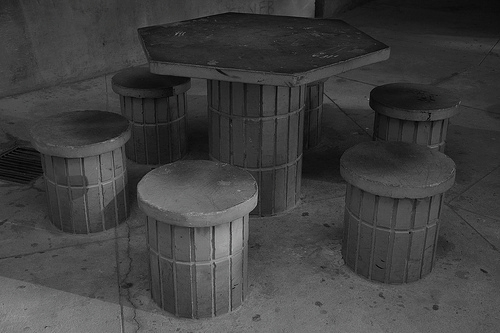
\includegraphics[scale=0.60, keepaspectratio=true]{img/imgs/11-lugares_estudar/-072.jpg}
    \end{figure}

    \item  \textbf{Arcádia (ou mesinhas do IEL):} A Arcádia é algumas mesas ao ar
    livre no IEL (Instituto de Estudos da Linguagem). Em horários de aula
    é silencioso, é um ambiente muito agradável e por ser ao ar livre, não fecha.
    Tem dois problemas: O grande fluxo de mulheres no local pode facilmente
    distraí-lo, principalmente se você as conhecer, e à noite enche de insetos (além
    da iluminação não ser das melhores). Às vezes, venta bastante e é ruim para
    estudar com folhas avulsas. Mas ainda assim é um ótimo local para estudar.

    \item  \textbf{Biblioteca do IFGW:} A biblioteca do IFGW (Instituto de Física
    Gleb Wataghin) é ótima para dias de calor, por ser super gelada (ar-condicionado
    mega-super-power!). Tem vantagem sobre as outras bibliotecas pelo fato das salas
    de estudo serem fora da biblioteca e por isso você não precisa deixar o seu
    material para entrar na sala de estudos. Recentemente reformada, agora conta
    com 6 baias para estudo em grupo e quantidade razoável de baias individuais, com tomadas
    onde você pode plugar seu notebook.

    \item  \textbf{BIMECC:} A biblioteca do IMECC tem poucos lugares, poucas
    mesas para estudo individual, os locais de estudo ficam dentro da biblioteca
    (você precisa guardar sua bolsa para entrar), não é muito gelada
    e o ambiente não é agradável, mas nela e na BAE é que você encontrará
    a maioria dos livros relacionados a computação.

    \item  \textbf{Outras bibliotecas:} Aventure-se por outras bibliotecas, como
    a da Economia, a da Pedago e a da Biologia e as conheça. Para aqueles que
    gostam (ou são obrigados) a estudar aos fins de semana a BC e as bibliotecas
    da Educação, da Economia, da Química, da Medicina, do IEL e da Geociências
    abrem aos sábados. Para saber os horários de funcionamento das bibliotecas,
    entre no site do SBU (\url{www.sbu.unicamp.brindex.php?link=30}).

    \item  \textbf{Bitolódromos:} Existem dois bitolódromos na Unicamp: O do IC
    e o da FEEC (coincidência interessante, né?). O do IC-3 é uma mesa grande
    com algumas cadeiras no antigo saguão de entrada. O da FEEC fica no fundo do
    prédio principal (qualquer veterano sabe onde é o bitolódromo, não tenha
    vergonha de perguntar). O da FEEC é maior, você se distrai menos porque não
    estão todos os seus colegas (mas várias outras pessoas estão) entrando
    e saindo de lá (embora os pica-fios sejam bastante barulhentos), e sempre
    você encontra gente que possa te ajudar. O do IC serve para quando você já
    estiver lá e com preguiça de ir à Elétrica, porque o da FEEC é muito melhor.

    \item  \textbf{Sala 316:} Outro alento para as madrugadas de estudo é a sala
    316 do IC-3, que fica aberta sempre, ou então, aberta facilmente com a chave
    em posse do guardinha. É uma sala com carteiras legais, lousa e ar
    condicionado, aliás, é muito boa para estudo em grupo (NABVS IMINENTVS) por
    causa da lousa.

    \begin{figure}[h!]
        \centering
        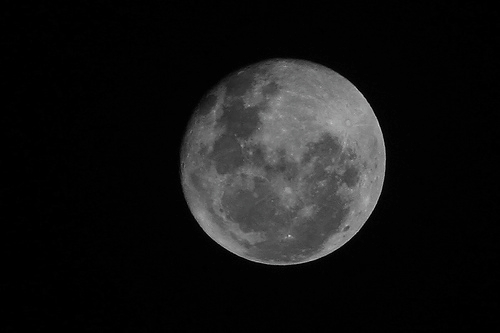
\includegraphics[scale=0.50, keepaspectratio=true]{img/imgs/11-lugares_estudar/-076.jpg}
    \end{figure}

    \item  \textbf{Sua casa:} Se você mora em uma república com pessoas da sua
    turma, vá fundo e estude em casa. Se você mora sozinho ou com caras de
    outros cursos/anos, mas se concentra bem em casa, também o faça. Caso
    contrário, estude na Unicamp. É muito fácil se distrair em casa. Você vai
    à geladeira, mexe no computador, lê outra coisa, deita na cama e dorme,
    entre outras coisas. Prefira estudar na Unicamp. Outra coisa, não seja
    egoísta, quando tiver oportunidade de estudar em grupo, prefira essa
    alternativa. Lembre-se que você não está mais no "cursinho", tente sempre
    pegar as dicas que a galera te dá, principalmente dos seus veteranos.

    \item  \textbf{Sala 363:} Vulgo salinha de estudo do IC. Pequena
    e aconchegante, tem mesas redondas, muito boas para estudo em grupo. Não
    costuma encher, por isso é bem tranquila. Tem uma estante com vários livros
    doados para uso livre.
\end{itemize}

\newpage
\section{Melhores banheiros}

Uma das maiores necessidades do ser humano pode ser potencializada se for
realizada num banheiro decente. Portanto, é muito importante que você saiba onde
ir. Alguns dos melhores banheiros da Unicamp são:

\begin{itemize}

    \item  \textbf{IC-3:} Geralmente estão limpos e utilizáveis. Mas fedem!
    Sempre com papel higiênico, é uma boa pedida na hora do apuro. Exceto nos
    finais de semana.

    \item  \textbf{IC-2:} Quase sempre estão limpos e utilizáveis e tem um odor
    melhor que os do IC-3. Só precisa tomar cuidado pois, as vezes, falta papel
    higiênico.

    \item  \textbf{FEEC:} Possui excelentes banheiros escondidos por lá. Procure
    bem!

    \item  \textbf{PB:} Os banheiros do segundo e do terceiro andar do Pavilhão
    Básico também são bons (especialmente os do terceiro andar, por quase não
    serem usados). Só tome cuidado, porque às vezes não tem papel higiênico.

    \begin{figure}[h!]
        \centering
        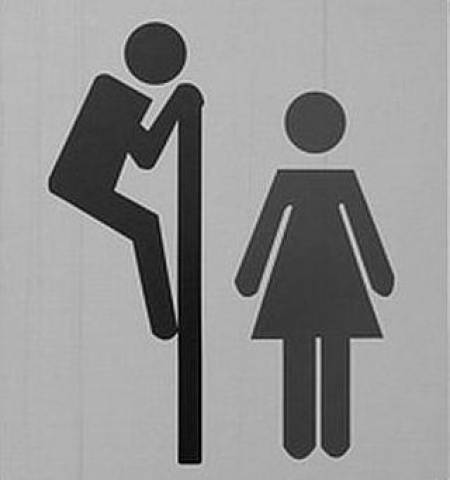
\includegraphics[scale=0.50, keepaspectratio=true]{img/imgs/12-melhores_banheiros/banheiro.jpg}
    \end{figure}

    \item  \textbf{FE:} A faculdade de educação tem poucos banheiros masculinos,
    mas estão entre os melhores da Unicamp pelo pouco uso.

    \item  \textbf{CB:} Estes banheiros ficam escondidos próximo às escadas do
    CB (no térreo). Se você tiver sorte de chegar bem após a limpeza, o banheiro
    estará em excelentes condições. Porém, na maior parte do tempo ele fica bem
    sujinho.

    \item  \textbf{DEQ:} Departamento de Eletrônica Quântica, no IFGW. Dizem que
    ninguém os usa.

    \item  \textbf{DRCC:} Departamento de Raios Cósmicos e Cronologia, no IFGW.
    Um dos melhores banheiros existentes na Unicamp (senão o melhor). Assim como
    os banheiros do DEQ, dizem que ninguém os usa.

    \item  \textbf{DFA:} Departamento de Física Aplicada, no IFGW. Os dois
    andares do departamento tem banheiros bons e utilizáveis, mas algumas vezes
    falta papel higiênico.

    \item  \textbf{IMECC:} Todos os três departamentos (andares) do IMECC tem
    banheiros bons e utilizáveis. Mas vez ou outra falta papel higiênico.
\end{itemize}


%%%%% Serviços da Unicamp
% Este arquivo .tex será incluído no arquivo .tex principal. Não é preciso
% declarar nenhum cabeçalho
\section{Serviços da Unicamp}
\subsection{Atendimento médico e odontológico -- CECOM}

A CSS é responsável pelo planejamento e execução de programas de saúde voltados
à comunidade universitária da Unicamp -- alunos, funcionários e docentes.
É responsável também pelo atendimento à saúde oral desta comunidade, incluindo
também os filhos menores de servidores que estejam devidamente matriculados nas
creches e escolas dos campi.

Em português, isso quer dizer que é um ``plano de saúde'' da Unicamp. Demora um
pouco (embora o pronto-socorro do CECOM seja bem mais rápido que o do HC), tem
burocracia, mas funciona. Você pode marcar consultas médicas e fazer exames.
O CECOM é localizado próximo ao HC. Para ir, é melhor pegar o Circular pois
é beeeeeem longe. De circular interno, peça para descer no CECOM. É o ponto
final ou o penúltimo dos circulares.

Caso você tenha Unimed, o Centro Médico, que fica perto da Unicamp, atende pela
Unimed. É mais rápido que o atendimento da Unicamp (CECOM ou SUS).

%%% Imagem do hospital
\begin{figure}[h!]
    \centering
    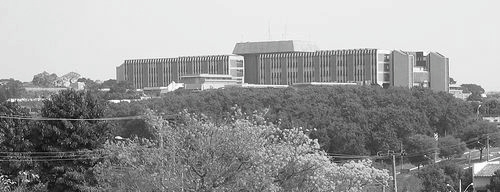
\includegraphics[scale=0.60, keepaspectratio=true]{img/imgs/13-servicos_unicamp/-077.jpg}
    \caption{Vista do Hospital de Clínicas da Unicamp}
\end{figure}


Para marcar consultas com Dentista, vá ao CECOM e pergunte onde que é. Isso é mais
fácil que você tentar entender lendo aqui. Basicamente é embaixo do CECOM, muito
fácil de chegar se alguém apontar com e dedo e dizer ``ali''. Funciona muito bem,
o atendimento é ótimo. A única burocracia é assistir uma palestra sobre doenças
da boca e escovação antes de poder marcar atendimento. Mas se você estiver com
dores eles te atendem na hora sem marcar consulta nem assistir palestra.

Para saber mais sobre o CECOM, vá ao site deles
(\url{www.unicamp.brcss/}).

\subsection{Hemocentro}

Essa é para quem é (ou para quem quer ser) doador de sangue. O centro de
hematologia e hemoterapia (hemocentro) é o órgão da Unicamp responsável pela
coleta e doação de sangue.
\begin{wrapfigure}{r}{0.2\textwidth}
    \vspace{-20pt}
    \begin{center}
    
\includegraphics[scale=0.14, keepaspectratio=true]{img/imgs/13-servicos_unicamp/doe_sangue2.jpg}
    \end{center}
    \vspace{-20pt}
\end{wrapfigure}
Qualquer pessoa pode aparecer no hemocentro para
fazer a doação de sangue. Basta estar com o RG e seguir um conjunto de normas
para a doação de sangue. Para saber mais sobre o processo, é só visitar a página
do hemocentro (\url{www.hemocentro.unicamp.br}).


O hemocentro também faz o projeto doador universitário, que consiste de unidades
móveis (ônibus) que param em alguns pontos do campus. Essas unidades fazem
a coleta do sangue. Alunos, professores e funcionários podem ir até essas
unidades móveis para fazer a doação. Para se informar melhor, é só visitar
a página do projeto
(\url{www.cecom.unicamp.brdoador_universitario/doador_universitario.html}).

O hemocentro fica localizado acima do HC (próxima ao CECOM). Portanto, se quiser
se deslocar até lá, como está escrito acima, é melhor usar o circular interno.

\subsection{Circular Interno e Ônibus Moradia}

O \textbf{Circular Interno} é um serviço de ônibus gratuito que dá voltas na Unicamp. Há duas linhas,
uma girando no sentido horário e outra no anti-horário. Só funciona até às 19h,
e a frequência maior é no horário de almoço. Bom para cobrir distâncias
como bandejão--IC, IC--FEEC, qualquer lugar--CECOM, qualquer lugar--FEAGRI,
FEAGRI--qualquer lugar. Quase todos os pontos têm os itinerários e os horários afixados.
Ele não costuma atrasar nem adiantar mais que 5 minutos, exceto no período de
férias.

O \textbf{Circular Noturno} é um ônibus que dá uma volta na Unicamp partindo do balão da
Avenida 1, passando pela BC, IQ, FEEC, IC e voltando para o balão da Avenida 1.
Os horários e o itinerário desse ônibus não estão nos pontos como os do Circular
Interno 1 e do 2. Ele funciona das 19h às 23h, a cada meia hora.

O \textbf{Ônibus Moradia} (ou ``Circular Externo'') dá uma volta na Unicamp partindo da BC, vai
para a Moradia e faz o caminho contrário. Ele também tem duas rotas alternativas
em horários específicos que cobrem as regiões da Avenida 1, Centro de Barão Geraldo
e Avenida 3. Os horários mais lotados do Ônibus Moradia são 8 da
manhã (sentido Moradia--Unicamp), horário de almoço (ambos os sentidos), horário
de jantar (ambos os sentidos) e o último horário (Unicamp--Moradia). Se puder
evitar esses horários, faça-o.

Todos os itinerários e horários detalhados dos serviços de ônibus podem ser
encontrados na página da Prefeitura da Unicamp: \url{prefeitura.unicamp.br}.

\subsection{SAE -- Serviço de Apoio ao Estudante}

O SAE (Serviço de Apoio ao Estudante), principal órgão de apoio ao estudante na
Unicamp, 
\begin{wrapfigure}{l}{0.22\textwidth}
    \vspace{-20pt}
    \begin{center}
    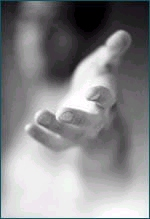
\includegraphics[scale=0.65, keepaspectratio=true]{img/imgs/13-servicos_unicamp/-081.jpg}
    \end{center}
    \vspace{-20pt}
\end{wrapfigure}
atua em várias frentes de assistência estudantil. Esta se dá por meio
do gerenciamento de bolsas-auxílio, assistência social e orientações
educacional, jurídica e psicológica, além de apoio a projetos acadêmicos
e sociais e programa de intercâmbio de estudantes no exterior. O SAE também
é responsável pela gestão de estágios na Universidade.

\begin{itemize}
\item  Localização: Prédio do Ciclo Básico, 3º piso (responsável pelo gerenciamento de convênios, estágios, bolsa-pesquisa e bolsa-empresa); e em frente a DAC (serviço social, responsável pelo gerenciamento de bolsas-auxílio).
\begin{itemize}
\item  Horário: Segunda a sexta, das 08h30 às 20h, no período letivo.
\item  Contato: sae [@] unicamp [.] br
\item  Site: \url{www.sae.unicamp.br}
\end{itemize}
\end{itemize}

\subsection{Bolsas-Auxílio}
\subsubsection{Moradia}

Criado em 1989, o Conjunto Residencial Universitário da Unicamp, tem por
finalidade garantir estadia gratuita e de qualidade para os estudantes que
passam por dificuldades sócio-econômicas.

Para saber mais sobre o processo seletivo entre no site da Moradia da Unicamp
(\url{www.prg.unicamp.brmoradia/index.html}).

\subsubsection{Bolsa Alimentação e Transporte}

Objetivo: Colaborar com o estudante de graduação e pós-graduação em dificuldade
sócio-econômica, nos itens alimentação e transporte.

Critérios para a seleção: Análise do questionário sócio-econômico devidamente
preenchido e documentado, e entrevista com a assistente social.

\subsubsection{Bolsa Trabalho}

Objetivo: Colaborar com o estudante de graduação em dificuldade sócio-econômica,
cuja família não tenha condições de mantê-lo na Universidade. Em contrapartida
o bolsista trabalhará 15 horas semanais em unidades da Unicamp, ou em grupos de
pesquisas, ou em grupos sociais, em horário compatível com o horário escolar.
E com a orientação de um professor.

Critérios para a seleção: Análise do questionário sócio-econômico devidamente
preenchido e documentado, e entrevista com a assistente social.

Alunos da pós não podem se candidatar à bolsa trabalho.

\subsubsection{Bolsa Emergência}

Objetivo: Atender os estudantes de graduação regularmente matriculados que
estejam passando por dificuldades econômicas emergenciais. Em contrapartida
o bolsista trabalhará 40 horas em unidades da Unicamp, compatível com o horário
escolar.

Procedimento: o candidato deverá enviar uma carta à Coordenação do SAE
solicitando o benefício e informando sobre os motivos. Preencher e entregar
devidamente documentado o questionário sócio-econômico e marcar entrevista com
a assistente social.

Critérios para seleção: Análise da solicitação, do questionário sócio-econômico
devidamente preenchido, documentado e entrevista com a assistente social.

Alunos da pós não podem se candidatar à bolsa emergência.

\subsubsection{Bolsa PAPI}

Busca incentivar a participação de alunos de graduação e de pós-graduação nas
mais diversas atividades da Unicamp, tais como no auxílio a eventos. Neste
programa, há a solicitação de estudantes por parte de alguma Unidade ou órgão da
Unicamp, que poderá indicar o nome do aluno ou deixar a critério do SAE para
fazê-lo.

\subsection{Assistência Jurídica}

Objetivo: Orientar os alunos nacionais ou estrangeiros de graduação ou
pós-graduação, na resolução de suas questões pessoais de cunho jurídico que
envolvam os ramos do Direito, principalmente os seguintes:

\begin{itemize}
\item  \textbf{Direito Civil:} contratos em geral; contratos de locação de imóvel/escritura de compromisso de venda e compra; acidentes de trânsito; reparação de dano; ação revisional de aluguel; separação judicial; divórcio; pensão alimentícia, etc.
\item  \textbf{Direito Penal:} violência contra a pessoa; lesões corporais; furto; roubo etc{\dots}
\item  \textbf{Direito do Trabalho:} caracterização de relação de emprego para os não registrados e direitos trabalhistas em geral (Normas da CLT).
\end{itemize}

Procedimento: O aluno deve dirigir-se pessoalmente ao SAE para obter os
esclarecimentos desejados.

Delitos de consumo, encaminhar ao SEDECON ou ao PROCON.

Com relação aos contratos de locação alertamos para algumas dicas importantes:

\begin{itemize}
\item  Jamais pagar qualquer valor antecipadamente (ex: ``taxas de reserva de imóvel'', ``taxa de contrato'', aluguel antecipado etc), ou fornecer títulos em garantia: (cheque pré-datado, nota promissória).
\item  Obter o maior número de informações possíveis relativas ao imóvel, proprietário(s), imobiliária, procuradores;
\item  Condições e valores para pagamento (aluguel e outros encargos ex.: Condomínio, IPTU, seguros etc, para uma real visualização do valor total a ser despendido).
\item  Sempre solicitar uma Minuta do contrato locação.
\item  Não assinar contrato ou qualquer outro documento antes de apresentá-lo para análise por um dos advogados da O.J. SAE.
\end{itemize}

\subsection{Orientação psicológica}

Objetivo: Prestar atendimento psicológico ao aluno de graduação, pós-graduação
e especial.

O Serviço de Orientação Psicológica do SAE funciona em associação com o Serviço
de Atendimento Psicológico e Psiquiátrico ao Estudante (SAPPE) do Departamento
de Psicologia Médica e Psiquiatria da FCM, desde a sua implantação, em 1987.

Funcionamento e informações:

\begin{itemize}
\item  Existem horários para consultas imediatas (ideais para quem está prestes a expulsar um amigo da república etc);
\item  O tratamento de longo prazo é obtido mediante uma palestra explicativa, um horário de atendimento individual e espera em uma lista de candidatos -- horários disponíveis e motivos especiais podem facilitar seu ingresso, mas lembre-se: não é porque aparentemente não parece importante o motivo pelo qual você procura ajuda que isso não deva ser levado a sério. Em alguns casos, apenas quatro seções são suficientes para a pessoa sair do tratamento (lembrando que ele pode ser interrompido a qualquer momento);
\item  Há possibilidade de tratamento em grupo terapêutico, psicoterapia individual, de família e de casal com uma das psicólogas da equipe. O grupo terapêutico é formado levando-se em conta que não devem haver pessoas muito próximas em sua formação, como condição de que o paciente tenha liberdade para falar de seus problemas com menos receio.
\end{itemize}

\subsection{Cadastro de veículos}

Para você poder entrar e sair da Unicamp sem ter de parar para receber e entregar
o papel de identificação do veículo você pode cadastrar seu carro junto
à Prefeitura do Campus. O cadastramento do veículo deverá ser feito diretamente
na Central de Informações (próximo ao Balão da avenida 1) de segunda
a sexta-feira das 09h às 17h.

Documentos necessários:

\begin{itemize}
\item  Identidade funcional (para funcionários/docentes), identidade estudantil para alunos, carta de apresentação da unidade para estagiários;
\item  Documento do veículo;
\item  Preenchimento de declaração.
\end{itemize}
Há possibilidade de se cadastrar até três veículos, com um custo de R\$ 5,00
para o segundo e de R\$ 10,00 para o terceiro veículo.

\subsection{Licenças de Software Gratuitas}

Bixo, agora que você é um computeiro de verdade, sua responsabilidade de não
usar software pirata é ainda maior. Afinal de contas, em poucos anos você pode
estar do lado dos desenvolvedores -- e não apenas consumidores -- de software.

A vantagem é que, por estar na Unicamp, você agora tem acesso a várias
licenças gratuitas de software proprietário especiais para estudantes.

O LMS (Laboratório Microsoft) ligado ao Instituto de Computação oferece download
gratuito de uma grande variedade de software da Microsoft, como o sistema
\textbf{Windows} e o ambiente de desenvolvimento integrado (leia-se: serve para
programar) \textbf{Visual Studio}. O Office não está disponível. Para mais informações
sobre como se cadastrar e baixar, acesse: \url{www.lms.ic.unicamp.br}.

A CTIC (Coordenadoria de Tecnologia da Informação e Comunicação) obtém licenças
de muitos pacotes de software e disponibiliza para a comunidade acadêmica, inclusive
alunos. As aplicações de computação científica \textbf{Wolfram Mathematica} e \textbf{MATLAB} estão disponíveis
gratuitamente. Para mais informações, acesse: \url{www.ctic.unicamp.br/softwares}.

A multinacional Autodesk oferece licenças de estudante gratuitas para muitos de
seus programas, incluindo o \textbf{AutoCAD} e a aplicação de modelagem
3D \textbf{Maya}. Para baixar, cadastre-se usando seu e-mail da DAC, do IC ou da
FEEC em \url{students.autodesk.com}.


%%%%% Agora eu tenho um email da Unicamp
% Este arquivo .tex será incluído no arquivo .tex principal. Não é preciso
% declarar nenhum cabeçalho

\section{Agora eu tenho um e-mail da Unicamp}

Ao ingressar num curso de computação, você recebe pelo menos duas contas de e-mail: do IC e da
DAC. Estes são os principais meios de comunicação da Universidade com você,
portanto fique esperto e não deixe de ler regularmente!

Para acessar o webmail do IC, o endereço é \url{webmail.students.ic.unicamp.br}.
O usuário e a senha são os mesmos do sistema Linux do IC, que você receberá nas
primeiras semanas de aula. Caso tenha dúvidas, dê uma passada na Secretaria de Graduação,
que fica no IC-2 (prédio ao lado das Artes Cênicas e para cima da Economia)
e pergunte!

Uma dica interessante, que muitas vezes passa
despercebida, é que no mesmo documento em que você recebe sua senha, vem indicado
um {\it alias} para o seu e-mail. Assim, você poderá utlizá-lo de
uma forma mais amigável, ao invés de ser somente o seu próprio RA, por 
exemplo:
\begin{verbatim}RA129873@students.ic.unicamp.br \end{verbatim} por 
\begin{verbatim}fransisco.silva@students.ic.unicamp.br \end{verbatim}

A DAC também dispõe um webmail para o aluno. O login é a primeira letra do nome
do aluno, seguido dos dígitos do RA. O e-mail da DAC também é útil. É nele que os
alunos são avisados sobre o período de matrícula, recebem os seus pedidos de
matrículas provisórias, avisos de desistências e trancamentos, além de informar
os alunos a respeito de eventos que acontecem na Unicamp, como feiras,
palestras, festivais, eleições. Na própria página da DAC
(\url{www.dac.unicamp.br}) você diretamente cria a sua senha e já pode
acessar o webmail dali mesmo.

Para a galera da Engenharia, ainda há o e-mail da FEEC, que muitos sequer ficam
sabendo que existe! Só um semestre ou até um ano depois vão até o SIFEEC retirar
seu login e senha. Ou então ficam sabendo só no segundo ou terceiro ano de curso
e aí há mais de 700 e-mails não lidos. Assim como o do IC, é muito
utilizado para divulgação de eventos, oportunidades de estágios e de iniciação
científica. Para utilizá-lo, você deve ir até a FEEC e procurar o SIFEEC, que
é o local responsável por isso. Fica no segundo andar do prédio de laboratórios
da FEEC (um com escadas amarelas). O endereço do webmail da FEEC
é \url{webmail.fee.unicamp.br} e a senha é a mesma do Linux da FEEC.

\begin{figure}[b!]
    \centering
    
\includegraphics[scale=0.50, keepaspectratio=true]{img/imgs/14-email_unicamp/-086.jpg}
\end{figure}
Você também pode redirecionar os e-mails que receber nas contas do IC, FEEC
e DAC para qualquer outra conta (no Gmail por exemplo). Para isso, siga as dicas
abaixo:

\subsection{Redirecionamento de e-mail da DAC}

Para efetuar o redirecionamento do e-mail institucional para outro e-mail, siga
os passos abaixo:

\begin{itemize}
\item  Acesse \url{www.dac.unicamp.br}
\item  Acesse Serviços On-line
\item  Acesse Alunos
\item  Clique em Acesso aos Serviços Acadêmicos
\item  Faça login
\item  Clique em Redirecionamento de Email
\end{itemize}

\subsection{Redirecionamento de e-mail da FEEC}

\begin{itemize}
\item  Acesse \url{webmail.fee.unicamp.br}
\item  Faça login
\item  Acesse Options
\item  Acesse Mail Forwarding
\end{itemize}

\subsection{Redirecionamento de e-mail do IC}

\begin{itemize}
\item  Acesse \url{webmail.students.ic.unicamp.br}
\item  Faça login
\item  Acesse Filtros
\item  Clique em Adicionar uma nova regra
\item  Em Condição, na primeira lista drop-down com a opção Header, escolha a opção All
\item  Em Ação, escolha Redirecionar para o seguinte endereço de e-mail
\end{itemize}

\subsection{Tenha uma conta no Gmail!}

Nós sabemos que é difícil. Muitas vezes você vem usando um serviço de e-mail
durante anos, seja ele Hotmail, Yahoo, Uol, Terra, Zipmail, e mudar é trabalhoso.
Mas confie na gente: agora vai ser mais fácil. Você está começando uma
vida nova na universidade, quando já tiver cadastrado seu endereço antigo
em vários serviços acadêmicos e divulgado entre os novos contatos que vai fazer,
será bem mais complicado.

Entre as vantagens do Gmail, podemos destacar:

\begin{itemize}
\item Muito espaço, nunca mais apague nada.
\item Visualização em threads, útil para acompanhar discussões.
\item Bom aplicativo para smartphones.
\item Filtros e marcadores infinitos para te ajudar.
\item Uma pesquisa que funciona.
\item Interface mais polida que as da concorrência.
\end{itemize}

Qualquer dúvida, novamente, procure um veterano!

Finalizando, não deixe de estar sempre informado sobre os acontecimentos ou
divulgações da Unicamp, do CACo, da AAACEC e da Conpec, essas três entidades
compostas por alunos de computação.


%%%%% Iniciação Científica
%%%%% Intercâmbio
%%%%% Eletivas e Proficiência
%%%%% Cuidado com CR e Reprovação
% Este arquivo tex vai ser incluído no arquivo tex principal, não pe preciso
% declarar nenhum cabeçalho

\section{Iniciação Científica}

A Iniciação Científica é um tempo para o aluno de graduação (você, no caso) ter
uma experiência acadêmica mais séria, sentir um pouco como é o clima de
pesquisa. Interessou? O que fazer? Calma, você mal entrou na Universidade.
Geralmente o que se faz é conversar com o professor da área com a qual você se
identifica mais (criptografia, teoria da computação, processamento de imagens,
inteligência artificial, etc), e ver se ele está desenvolvendo algum projeto
interessante naquela área, ou propor para ele alguma idéia sua original mesmo.
Depois você começa a estudar para redigir um projeto e encaminhar para alguma
instituição de fomento à pesquisa (CNPq ou FAPESP), pedindo uma bolsa de
Iniciação Científica. A FAPESP paga R\$502,80 e aceita pedidos de bolsa em
qualquer período do ano. O CNPq paga aproximadamente R\$360,00, e o período para
inscrição de projetos é geralmente em junho e novembro. No primeiro semestre
geralmente é bem mais difícil achar algum professor da área que você se
interessa, aliás, é bem difícil saber a área com a qual você se identifica, pois
você mal começou o curso e não conhece muito do que se estuda em Computação,
muito menos os professores. Mas tenha paciência, agora parece tudo muito
complicado e complexo, mas com o tempo, as coisas vão ficando mais simples. Se
você realmente tiver uma sede insaciável de conhecer o meio da pesquisa, procure
o seu professor de MC102, ele pode te orientar a respeito.

Outra coisa interessante a respeito da Iniciação Científica é que, se você
conseguir bolsa (o que não é muito difícil), pode pegar a disciplina MC040
e posteriormente MC041 (2 semestres), cada uma com 6 créditos, e geralmente se
tira notas altas nessas disciplinas. Ou seja, são 12 créditos praticamente "de
bandeja" para aumentar o seu CR, ou ajudar a recuperá-lo, caso esteja no fundo
do poço. Note bem as aspas. Os trabalhos de Iniciação Científica geralmente
consomem muito tempo de estudo e dedicação, não vá pensando que é moleza não.

Na FEEC você pode conseguir as matérias de Iniciação (EA002 até EA005) mesmo sem
bolsa, mas você ainda assim vai precisar de um orientador. Lá a Iniciação
Científica também substitui o estágio, mas não tem equivalência com as do IC.

\section{Intercâmbio}

Como assim? Acabei de sair da minha cidade natal, do aconchego do meu lar e você
vem me falar de sair do país? Calma, calminha{\dots} Não é para agora, mas é bom
ir se preparando {\dots} Falando sério, uma introdução sobre intercâmbios.
A Unicamp hoje, junto com a USP, é uma das universidades brasileiras que tem
maior prestígio fora do país e o Cori (Cooperação Internacional), IC e FEEC tem
vários acordos bilaterais de intercâmbio. Então para você que quer dar um salto
em algum idioma, conhecer outras culturas e sentir na pele a aventura de ser
estrangeiro, comece a se preparar desde já.

A primeira coisa é escolher uma língua. Pois, mesmo o inglês sendo a língua que
se fala no mundo, não é 100\% da população do país de destino que fala o inglês
corretamente, então pense em começar a estudar a língua do país em que pretende
ir no seu intercâmbio. Hoje a maior parte dos computeiros vai para França,
Alemanha e países hispanofônicos, logo pensar em fazer francês, alemão ou
espanhol é uma boa pedida e com chances de facilitar sua aceitação do pedido de
intercâmbio. Existem também bolsas para estudos na Itália, então aprender
italiano pode ser uma boa alternativa. Ter um bom nível de inglês também ajuda
no processo seletivo e, claro, inglês não faz mal a ninguém (ainda mais, a nós
do ramo de tecnologia)!

Para onde ir? Grande questão! Vou citar o caso dos EC03: de 90 alunos, 10 alunos
foram estudar/estagiar fora! Destes, 6 foram para França, 1 para Portugal,
1 para Itália, 1 para Eslovênia e 1 para Argentina.

A França hoje recebe grande numero de estudantes de computação, dado acordos que
a FEEC tem com os INSA's e com as écoles Centrales e também graças a bolsas de
estudo oferecidas pela Capes e pelo governo francês. Mas não significa que
a França seja seu destino certo, no site do CORI existem oportunidades para ir
para, além dos países já citados, Japão, América Latina, Alemanha, Espanha, etc.
Muitos com boas bolsas de estudo ou com incentivos que valem a pena caso você
tenha um pouco de grana para se sustentar no inicio. Visite sempre o site da
CORI e participe das reuniões que ela faz, ficar ligado é a chave para conseguir
encontrar uma boa oportunidade. Existem outras opções de intercâmbio como
o AIESEC que promove um intercâmbio para estágios no exterior, se seu interesse
é mais profissional, procure se informar.

Mas vale a pena? Poxa, vou atrasar meu curso, ficarei deslocado de turma, vou
ficar em um país estranho, para quê? Acho que não vale a pena{\dots}

{\dots}Ledo engano, ledo engano{\dots}

Vamos começar pelos motivos profissionais : ter no currículo que você fala uma
lingua estrangeira fluentemente devido a sua imersão no país é algo muito
valorizado pelas empresas, além do fato que o pessoal do RH vai ver que você tem
capacidade de se virar sozinho, uma vez que não é tão óbvio sair do país
e recomeçar sua vida fora. Você não atrasará tanto seu curso, pois a Unicamp
conta com um sistema de equivalências de matérias e se você escolher bem pode
fazer matérias que serão convalidadas na Unicamp. Agora, o que realmente
é importante! Você está na faculdade, está na hora de deixar o colo da mamãe
e partir para o mundo{\dots} a experiência de conhecer outras culturas, criar
laços de amizade (ou mesmo algo mais) internacionais, viajar por terras
desconhecidas não tem preço!!! Pense que é no seu tempo de facul que terá
oportunidade de fazer uma aventura destas, não desperdice{\dots}

Se você abriu um sorriso e pensa que está preparado para sair do país{\dots}
comece a estudar, garoto! Não que, ter uma boa nota seja a única forma de
conseguir uma vaga em uma bolsa de estudos, mas com certeza é a mais fácil.
Busque "atirar em todas as frentes", mantenha seu CR num bom nível, busque
conhecer organismos como AIESEC e procure grupos de trabalho (no IC existem
vários) que podem levar alunos ao exterior. Boa sorte!

Se você realmente se interessou, ai vão uns links com mais informações:

\begin{itemize}
\item  AIESEC: \url{http://www.aiesec.org/brazil/}
\item  CORI: \url{http://www.cori.unicamp.br/}
\end{itemize}

Fique atento aos e-mails que você receberá do IC e da FEEC. Muitos deles são sobre programas de intercâmbio.

\section{Eletivas e Proficiência}

A UNICAMP oferece a seus alunos a oportunidade de personalizar seu currículo de
acordo com seu interesse por meio das disciplinas eletivas. Ao contrário das
disciplinas do núcleo comum, você pode escolher a matéria que vai cursar. Alguns
créditos podem ser cumpridos com qualquer disciplina oferecida pela
universidade, outros estão restritos a um determinado conjunto (para mais
detalhes, consulte seu catálogo no
\href{http://www.dac.unicamp.br/portal/grad/catalogos/index.html}{site da DAC},
na página destinada à Graduação).

Mas não se esqueça de que com um grande poder vem uma grande responsabilidade!
A UNICAMP lhe dá liberdade para escolher o melhor jeito de se preparar para seu
futuro, e espera que você saiba o que fazer com ela. Você pode socializar com
outros cursos, aprender uma língua estrangeira, assistir a seminários ou obter
um certificado de estudos na FEEC ou no IC.

Muitas pessoas, especialmente nos cursos de computação, fazem proficiência em
línguas, em alguns casos para evitar o jubilamento, outros para não ter que
passar mais um semestre na faculdade. Apesar de registrar a familiaridade do
aluno com uma outra língua em sua integralização, essa prática não enriquece
a graduação de nenhum estudante que faça tal escolha. Além disso, muitos bixos
arrependem-se de terem feito a prova e perdido preferência na hora de pegar uma
disciplina interessante, podendo até mesmo não conseguir se matricular.

Converse com seus amigos e veteranos para descobrir o melhor jeito de usufruir
dessa liberdade que poucas universidades oferecem! Dificilmente você não
encontrará algo com o qual se identifica ou que não ensine lições interessantes.

\section{Cuidado com CR e Reprovação}

Durante o curso você vai ouvir que se preocupar com seu CR é bobagem, que
estudar para tirar nota não leva a lugar nenhum, que depois de formado não é seu
CR que te colocará no mercado de trabalho, etc. Cuidado, a sua única opção de
vida após formado não é trabalhar numa empresa, e preste atenção "após formado"
não significa durante o curso.

Durante o curso você vai ter a possibilidade de participar de várias atividades
acadêmicas e algumas delas vão exigir bom aproveitamento acadêmico do aluno, por
exemplo, para se candidatar a monitor de uma disciplina é exigido do aluno um CR
>= 0,7. Isto significa que sua média de notas das disciplinas cursadas até
aquele momento deve ser maior ou igual a 7,0. Para pleitear uma bolsa de
iniciação científica, onde há concorrência entre alunos do país todo, também
será exigido bom aproveitamento, assim como para uma bolsa de mestrado. Caso
você não saiba, mestrado faz parte da pós-graduação, ou seja, o seu CR vai te
influenciar até após formado.

Cuidado também com a reprovação, há instituições, como a FAPESP (Fundação de
Amparo à Pesquisa do Estado de São Paulo) que é a maior fomentadora de pesquisas
do estado de São Paulo e que paga os maiores valores de bolsas do país, que te
exclui de qualquer disputa só por ter uma reprovação no seu histórico escolar da
graduação. Não te exclui oficialmente, mas como é muito concorrido por ser
a melhor pagadora, se seu nome for para o final da lista por causa da reprovação
pode considerar-se excluído da disputa.

Parece óbvio, quem estuda tira boas notas, mas até você aprender a estudar como
a universidade exige pode demorar um pouco e há pessoas que nunca aprendem.

Há certos períodos (semestres) quando você já estiver mais avançado no curso em
que poderá sentir-se à vontade para desistir de uma disciplina em que esteja
matriculado, deixando para completá-la posteriormente. Quando você fizer isso há
a possibilidade de desistir da disciplina, se desmatriculando oficialmente dela.
Mas há pessoas que simplesmente deixam de cursar a disciplina, reprovando por
nota e falta e ficando com uma nota baixa em seu histórico. Cuidado com isso,
pode ser frustrante para você no futuro. Por isso se for desistir de cursar uma
disciplina após matriculado, sempre peça a desistência e tente não reprovar.

Lembre-se de que 4 ou 5 anos é muito tempo, você pode mudar de ideia a qualquer
momento sobre o que pretende fazer no futuro.


%%%%% Grupos e Entidades da Unicamp
% Este arquivo .tex será incluído no arquivo .tex principal. Não é preciso
% declarar nenhum cabeçalho

\section{Grupos e Entidades da Unicamp}

\subsection{Alumni Computação Unicamp}

\begin{figure}[H]
    \centering
    
\includegraphics[scale=0.40]{img/alumni_comp.png}
\end{figure}

Alumni é o nome dado a ex-alunos de uma universidade. Por extensão,
alumni também é o nome de organizações sem fins lucrativos motivadas em manter
o relacionamento entre a universidade e os ex-alunos e o destes entre si, servindo como uma rede
de contatos profissionais. A comunicação entre alunos, ex-alunos e professores proporciona um compartilhamento de experiência e informações, que contribuem para uma diferenciação acadêmica, cultural e profissional.

O \textbf{Alumni Computação Unicamp} é uma forma de manter todos que passaram
pelo melhor curso de computação da América Latina conectados -- tanto alunos
quanto ex-alunos. Atualmente o Alumni conta com uma página no Facebook (\url{fb.com/AlumniComputacaoUnicamp}), que reúne os grupos das turmas que passaram pela Computação, com o objetivo de atingir o maior número de alunos e ex-alunos.

Participe do grupo de sua turma, convide seus amigos a curtirem a página, envie sugestões e contribua para essa ideia!

\subsection{ARU}

\subsubsection{O que é a ARU – Associação de Repúblicas da Unicamp?}

\begin{figure}[H]
    \centering
    
\includegraphics[scale=0.40]{img/aru.png}
\end{figure}

Idealizada em 2008, a ARU é a entidade que representa as Repúblicas Associadas de
Barão Geraldo.  Tem como meta prestar apoio a elas, zelar pela sua segurança
e bem estar com toda a vizinhança, como também servir de espaço
para discutir os problemas apresentados em reuniões.

\begin{figure}[H]
    \centering
    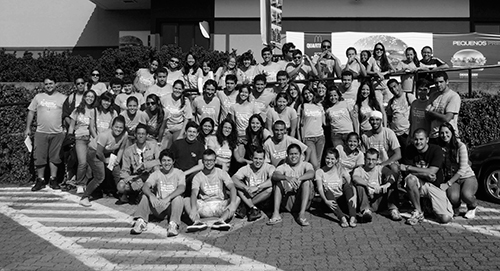
\includegraphics[scale=0.40]{img/aru_foto.jpg}
\end{figure}

Além de entregar no começo do ano um manual para os bixos contendo informações
sobre as Repúblicas Associadas, a ARU também realiza vários eventos, os quais
têm o objetivo de integrar e divertir os moradores de repúblicas. Alguns deles
são: a \textbf{Alcorrida}, a \textbf{Campanha do Agasalho},
o \textbf{EntortaRep}, e, principalmente, o \textbf{InterReps}.

\subsubsection{Contato}

\begin{compactitemize}
    \item Site: \url{republicasunicamp.com.br}
    \item E-mail: \email{contato@republicasunicamp.com.br}
    \item Facebook: \url{fb.com/republicasunicamp}
\end{compactitemize}

\subsection{Competições de programação}

Curte programar? Nunca programou mas está gostando de MC102? Já brincou de
Olimpíada naquelas provas com direito a medalha? Vá fundo!

Para os bixos que ingressaram direto do ensino médio existe a
\textbf{OBI -- Olimpíada Brasileira de Informática}, logo no primeiro semestre.
Anualmente, muitos alunos do IC, tanto da Ciência como da Engenharia, ganham
premiações nessa competição. O site dela é \url{olimpiada.ic.unicamp.br}.
Visite-o para mais informações.

\begin{figure}[h!]
    \centering
    
\includegraphics[scale=0.40, keepaspectratio=true]{img/maratona.png}
\end{figure}

Mas a principal competição para alunos de ensino superior é a
\textbf{Maratona de Programação}, que consiste de problemas mais difíceis e é
feita em equipes de três alunos. A Unicamp tem grande tradição nessa competição,
tendo levado equipes para a competição mundial (a ACM-ICPC) em 1996, 2000, 2002,
2003, 2004, 2007, 2009 e 2012.

Além de brilhar no currículo, é muito divertido competir, e a experiência obtida
nos treinamentos tem levado muitos maratonistas a empresas como Google,
Microsoft e Facebook.

Para participar dos treinamentos para a Maratona que acontecem na Unicamp,
inscreva-se no grupo \url{groups.google.com/group/maratona_unicamp}.

\subsection{DCE}

Criado em 1978, o DCE Unicamp (Diretório Central dos Estudantes) é a entidade que
representa todos os estudantes de graduação da Universidade, articulando
e organizando o movimento estudantil (ME).

Cabe ao DCE representar o conjunto dos
estudantes em todos os espaços dentro e fora da universidade, diante das mais
diversas entidades (reitoria, sindicatos, DCEs de outras universidades, centros
acadêmicos, associações etc.) e movimentos sociais.

Como articulador do ME, cabe ao DCE organizar os estudantes na luta por uma
educação superior realmente pública, gratuita e de qualidade. Para tanto,
é papel fundamental do DCE propor, juntamente com os centros acadêmicos,
discussões políticas que extrapolem os nossos currículos e o nosso dia a dia.
Além disso, o DCE deve propor ações que vão ao encontro das reivindicações
estudantis, de forma que elas sejam levadas e cobradas da reitoria ou até mesmo
do governo.

O DCE esteve envolvido em várias conquistas dos estudantes, das quais se
destacam algumas lutas históricas: a construção da moradia estudantil; a melhoria
de estrutura para cursos noturnos, que tornou acessível para esse período
bibliotecas, xérox, laboratórios e secretarias de graduação; a reunião semestral
para avaliação de curso; o não-aumento do preço do bandejão; uma seleção mais
justa para as vagas na moradia; entre diversas outras. Além disso, o DCE teve
participação em importantes lutas sociais que extrapolam o âmbito da Unicamp,
como a organização do Plebiscito contra a Alca e do Plebiscito contra o Provão;
a luta por mais verbas para a educação no estado de São Paulo; diversas lutas
pela qualidade do ensino e manutenção de direitos dos estudantes em outras
universidades como na UNIP, UNIMEP, FUPPESP etc.

No fim do ano, há eleições para definir qual
a chapa que comandará a entidade no ano seguinte, juntamente com eleições para
representação discente no Consu e na CCG. É muito importante a participação dos
alunos nessas eleições.

Não deixe de participar da Calourada Integrada organizada pelo DCE e centros
acadêmicos e das reuniões do DCE, que acontecem na sede próxima ao Bandejão.

\begin{compactitemize}
\item  Telefone: (19) 3521-7910 / (19) 3521-7042.
\item  E-mail: \email{dceunicamp@gmail.com}.
\item  Site: \url{dceunicamp.org.br}.
\end{compactitemize}

\subsection{Gamux}

O Gamux (Grupo de Pesquisa e Desenvolvimento de Jogos da Unicamp), composto por
computeiros e alunos do IA (Instituto de Artes), é uma ótima oportunidade para
quem tiver curiosidade de saber como são feitos os jogos eletrônicos.

Fique atento, eles costumam organizar ciclos de palestras e eventos relacionados
a desenvolvimento de jogos.

Mas não precisa esperar até lá! Apareça no LMS (Laboratório da Microsoft,
próximo as mesinhas do IC3) ou entre no grupo de e-mail.

\begin{compactitemize}
\item  Site: \url{gamux.com.br}
\item  Lista de discussão: \url{groups.google.com/group/gamedev_unicamp}
\end{compactitemize}

\subsection{GPSL}

O \textbf{GPSL -- Grupo Pró Software Livre} é aberto para alunos de todas as
unidades e para a comunidade. Sua missão é promover o uso e o desenvolvimento do
software livre.

Muitas instituições educacionais utilizam software proprietário e a Unicamp não
é exceção. São poucas as unidades que usam software livre e é muito fácil se
formar sem sequer saber da existência ou ter qualquer experiência com algo
diferente do software proprietário vigente.

\begin{figure}[h!]
    \centering
    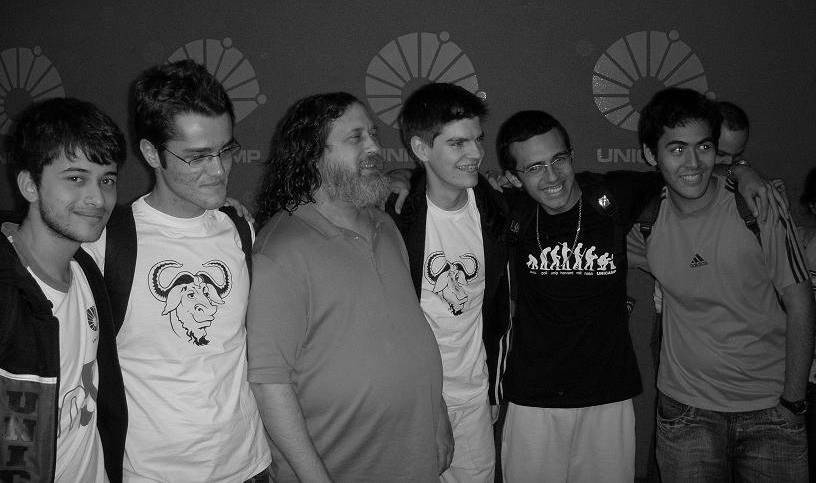
\includegraphics[scale=0.36, keepaspectratio=true]{img/imgs/18-grupos_entidades/stallman2.JPG}
    \caption{Richard Stallman em vista à Unicamp}
\end{figure}

O GPSL é um espaço para refletir sobre a predominância do software proprietário,
cujo uso muitas vezes é imposto, inclusive pela universidade, a ética por trás
disso e os efeitos sociais decorrentes. É também um espaço para se articular e
pensar em formas de ação, que podem envolver desde a educação e a
conscientização dos usuários de computadores até o próprio desenvolvimento de
software livre. O GPSL também pensa sobre questões de mercado e econômicas
relacionadas ao software livre.

Tradicionalmente, o GPSL organiza, com o apoio do CACo, o \textbf{Curso de
GNU/Linux Para os Bixos}. Este curso, como o próprio nome diz, é voltado para os
bixos como você que ingressam nos cursos de computação, embora seja aberto
também a veteranos. O objetivo é ensinar o básico do sistema operacional
GNU/Linux para você se virar nas matérias de computação do primeiro semestre.
Ele geralmente é ministrado em abril, mas não existe data fixa. Mas não se
preocupe, você será avisado na sala de aula por um veterano e receberá um
comunicado pelo seu e-mail do IC.

Para participar das discussões do GPSL, inscreva-se no grupo de e-mail em
\url{groups.google.com/group/gpsl-unicamp}.

\subsection{MTE}

\begin{figure}[H]
    \centering
    
\includegraphics[scale=0.40]{img/mte.png}
\end{figure}

O \textbf{MTE -- Mercado de Trabalho em Engenharia} é uma entidade estudantil que visa colocar o aluno da Unicamp em
contato mais próximo com o mercado de trabalho e com as possibilidades que ele
proporciona, mostrando as diferentes áreas de atuação de um engenheiro.

A participação no MTE desenvolve habilidades como networking, oratória, expressão, empreendedorismo, gestão e diversas outras.

A estrutura do MTE é dividida em três pilares:

\begin{description}
\item[Oportunidades:] responsável por atividades como visitas técnicas e captação de treinamentos e palestras.
\item[Desenvolvimento:] responsável por atividades como English Meeting (encontros de conversação em inglês), Teia do Conhecimento (treinamentos dados por algum dos membros) e Ciclo de Oratória (ciclos com foco em melhoria de expressão).
\item[Orientação e Carreira:] responsável pela estruturação pessoal e profissional dos membros realizando feedbacks, atividades de consultoria, de motivação, entrevista com profissionais e confraternizações.
\end{description}

Além da participação em um dos pilares, alguns membros participam da diretoria administrativo-financeira e, para completar, participam da realização de dois principais eventos: o EMC (Estudante e Mercado Conectados) que conta com visitas técnicas e palestras e o ArenaMTE, um desafio universitário de resolução de cases.

Para mais informações sobre o MTE e seu processo seletivo, acesse
\url{mte.org.br}.

\subsection{Rádio Muda}

Você provavelmente nunca viu nada do tipo na sua vida. Uma rádio na qual
qualquer ser humano pode fazer o seu programa tranquilamente, sem burocracias
(tendo espaço na grade de horários, lógico).

A Rádio Muda fica embaixo da caixa d'água (carinhosamente apelidada de Pau do
Zeferino) que fica perto do Teatro de Arena, bem em frente à BC (Biblioteca
Central).

Se você só quiser ouvir a muda, 88,5 MHz no seu rádio (em Barão Geraldo ou
Paulínia) ou pela Internet, através do site \url{muda.radiolivre.org}.

\subsection{Curso Exato}

O Curso Exato é um projeto da Pró-Reitoria de Extensão e Assuntos Comunitários
da Unicamp criado em 2008 por alunos de graduação, com a finalidade de explorar
o potencial e a capacidade dos alunos de se expressarem, de raciocinarem
logicamente e de compreenderem o mundo que os cerca, por meio de aulas de Língua
Portuguesa, Matemática, Física e Química.

Os professores do curso são alunos de graduação e pós-graduação da universidade
e o público alvo é constituído por alunos da rede pública de ensino com
disposição e interesse para aprender.

As aulas são realizadas no período noturno, das 19h15 às 22h30, de segunda
a quinta-feira, no campus da universidade.

\begin{compactitemize}
\item Site: \url{cursoexato.com.br}
\item Facebook: \url{fb.com/curso.exato}
\item E-mail: \email{curso.exato@gmail.com}
\end{compactitemize}

\subsection{Grupos Religiosos}

\subsubsection{ABU -- Aliança Bíblica Universitária}

Grupo evangélico não ligado a nenhuma denominação, organiza várias reuniões
e grupos de discussões e é filiado à Aliança Bíblica Universitária do Brasil
(\url{abub.org.br}).

\begin{compactitemize}
\item Site: \url{abucampinas.org}
\item E-mail: \email{contato@abucampinas.org} ou
        \email{abucamp_co@yahoogrupos.com.br}
\item Telefone: (19) 3289-2823
\end{compactitemize}

\subsubsection{Pastoral Universitária}

Grupo católico que se reúne semanalmente para estudar textos (bíblicos ou não),
livros, documentos, aprofundar a fé e promover a integração e união de seus
participantes. A Pastoral Universitária também organiza grupos de preparação
para Primeira Comunhão e Crisma, além de duas Missas semanais e Grupos de Oração
Universitários (GOUs). As Missas são realizadas às terças (18h) e às
quintas (12h15), sempre no PB04. Os GOUs acontecem às terças (12h15) e
nas quintas (18h), também no PB04.

\begin{compactitemize}
\item Site: \url{sites.google.com/site/pastoralunicamp}
\item E-mail: \email{pastoralunicamp@gmail.com}
\end{compactitemize}

\newpage
\section{Conpec}

\begin{figure}[H]
    \centering
    
\includegraphics[scale=0.40]{img/conpec.png}
\end{figure}

A Conpec é a empresa júnior dos cursos de Ciência e Engenharia de Computação da
Unicamp.

Nela você tem a oportunidade de aplicar os conhecimentos teóricos
adquiridos em sua vida acadêmica em uma situação real, de mercado, com clientes,
prazos e soluções reais. É uma chance ainda de aprender sobre aspectos de mercado de trabalho que você
nunca veria na faculdade, como marketing, finanças, planejamento, trabalho em equipe e liderança,
indispensáveis considerando-se que o perfil empreendedor é cada vez mais exigido do profissional de
computação. Muitos membros e ex-membros da Conpec usam os
conhecimentos adquiridos na empresa não só como um adicional ao buscar uma vaga
no mercado de trabalho, mas também para montar suas próprias empresas ou em
serviços não ligados diretamente à computação, como consultorias estratégicas.

Além disso, a Conpec é uma excelente oportunidade para conhecer os seus colegas
de curso, sejam veteranos ou bixos, pessoas de outros cursos e até mesmo de fora da
Unicamp, uma vez que há diversas empresas juniores espalhadas pelas universidades de São Paulo e do Brasil. É ainda uma grande chance para perder a inibição de falar em
público e aperfeiçoar sua capacidade de expor opiniões, além de aprender como
agir em um ambiente profissional.

\begin{figure}[H]
    \centering
    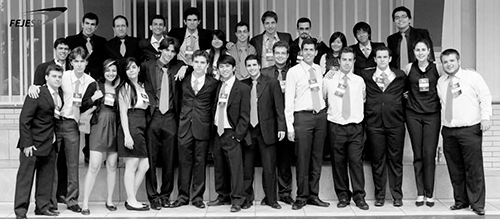
\includegraphics[scale=0.40]{img/conpec_foto.jpg}
\end{figure}

Para fazer parte da Conpec, fique atento à data da palestra de apresentação do
processo seletivo, que ocorre no início do ano.

Para saber mais sobre a empresa visite o site \url{conpec.com.br} ou
tire suas dúvidas mandando um e-mail para \email{conpec@conpec.com.br}.

\newpage
\section{Atlética -- AAACEC}

Assim como em outras unidades de ensino da Unicamp, o Instituto de Computação
(IC) e a Faculdade de Engenharia Elétrica e de Computação (FEEC) tem sua
entidade que promove a prática de eventos desportivos entre os membros da
graduação e da pós-graduação: A Associação Atlética Acadêmica da Ciência
e Engenharia da Computação, mais conhecida como AAACEC, ou simplesmente
\textbf{Atlética}. A AAACEC é uma entidade sem fins lucrativos, que tem uma
diretoria composta por alunos da computação, eleita a cada ano pelos alunos
dos cursos de Engenharia e Ciência da Computação e pós-graduandos vinculados ao IC.

A AAACEC é a entidade responsável pela participação da Computação em competições
esportivas, tanto dentro da Unicamp (Calouríadas, Interanos, Olimpíadas) como
com faculdades de outras cidades (Intercomp),
\begin{figure}[h!]
    \vspace{-10pt}
    \centering
    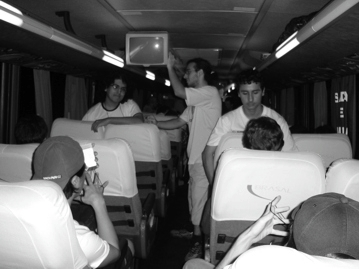
\includegraphics[scale=0.75, keepaspectratio=true]{img/imgs/20-aaacec/-096.jpg}
    \vspace{-10pt}
\end{figure}
competições essas que costumam
acontecer uma vez a cada ano. A fim de possibilitar essa participação, a AAACEC,
além de se encarregar das inscrições e organização, promove treinos regulares de
basquete, vôlei, handball e futsal, e disponibiliza o material (bolas, redes,
etc.) para a prática de tais esportes. A AAACEC se encarrega da reserva e/ou
locação de quadras para a realização dos treinos e competições em que isso se
fizer necessário. Os treinos são semanais e oferecidos para as modalidades
masculina e feminina, de forma que qualquer associado da Atlética pode
participar.

\subsection{Como, então, se associar à AAACEC?}

No caso dos recém-ingressantes, o jeito mais simples é comprando o KIT BIXO,
organizado pela própria AAACEC, contendo camiseta, caneca e outros produtos da
Atlética. Com ele, o calouro torna-se sócio e pode usufruir livremente de todos
os jogos e/ou eventos que a AAACEC venha a organizar pelo resto de sua vida.

Quem não comprar o Kit Bixo no primeiro ano, pode se associar mais tarde com o
pagamento de uma taxa de associação. Além do Kit Bixo, a AAACEC tem diversos
produtos que podem ser comprados por qualquer associado durante todo o curso,
como camisetas, blusas, agasalhos, adesivos, chaveiros, mouse-pads, entre
outros.

\subsection{E para quem vai o dinheiro da compra do kit bixo e dos demais produtos?}

A AAACEC promove a integração entre os alunos, e a realização de experiências
sociais e esportivas:

\begin{itemize}
\item  \textbf{A famosa Choppada Comp/Enf} (gratuita para os bixos)
\item  \textbf{Churrascos}
\item  \textbf{Torneios Esportivos:}
\begin{itemize}
\item  \textit{Internos} (Torneio início, Calouríadas, InterAnos, Olimpíadas)
\item  \textit{Externos} (Intercomp, UniSinos)
\end{itemize}
\begin{figure}[h!]
    \vspace{-10pt}
    \centering
    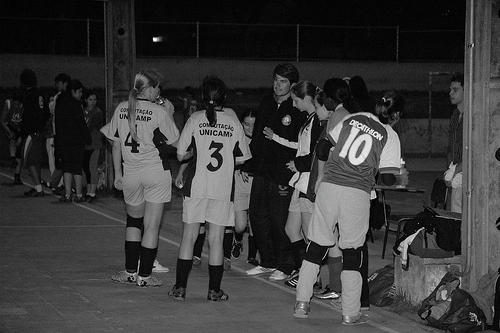
\includegraphics[scale=0.58, keepaspectratio=true]{img/imgs/20-aaacec/-100.jpg}
    \vspace{-10pt}
\end{figure}
\item  \textbf{Festas} (Muitas delas em união com outros cursos, promovendo ainda maior integração)
\end{itemize}

Para tudo isso, é necessário capital, que é obtido com muito trabalho da
Diretoria com a venda dos Kits Bixo e produtos.

É importante lembrar que a diretoria não tem remuneração alguma: Os diretores
trabalham pelo ideal comum de fazer a Computação crescer, e, consequentemente,
ganhar experiência de organização de eventos e pessoas, aprendizado de valor
inestimável, tanto na vida profissional como social.

A AAACEC busca fortalecer, acima de tudo, o nome do curso de Computação da
Unicamp, enaltecendo nossas qualidades dentro e fora da Universidade! Orgulho de
ser Computação Unicamp!!

Faça parte você também dessa integração! Associe-se à AAACEC!

As diretorias anteriores da AAACEC podem ser vistas em:
\url{aaacec.com/diretoria}

\subsection{Contato}

Não hesite em tirar dúvidas ou enviar sugestões!

\begin{compactitemize}
\item  E-mail: \email{aaacec@ic.unicamp.br}
\item  Site: \url{aaacec.com}
\end{compactitemize}

\subsection{Atendimento}

Ainda não há uma definição para este semestre, mas provavelmente o atendimento
será de segunda a sexta das 12h30m às 13h30m e segunda a quinta das 18h-19h

\subsection{Reuniões}

As reuniões serão marcadas no começo do semestre. Elas são realizadas num dia
letivo às 12h no IC-3.

\subsection{Bateria Valorosa}

Criada em 1998, a bateria Valorosa é umas das melhores baterias da Unicamp.

Durante o ano, ela participa de diversos eventos, como o Intercomp, Interbatuc,
UPA, e apoiando nossos atletas em jogos internos. Também somos convidados por
outros cursos para tocar em seus jogos.

A Bateria realiza ensaios semanais, dos quais estão todos convidados a
participar.

Esperamos que muitos bixos participem, e para isso basta comparecer aos ensaios,
lembrando que não é necessário saber tocar nenhum instrumento. TODOS que
quiserem aprender serão muito bem-vindos na bateria!

\newpage
\section{CACo -- Centro Acadêmico da Computação}

\begin{figure}[H]
    \centering
    
\includegraphics[scale=0.37]{img/caco/logo.png}
\end{figure}

Bixo, o CACo é o seu centro acadêmico. Um CA é uma entidade estudantil que, em
linhas gerais, deve trabalhar para garantir os interesses dos estudantes e
melhorar o curso e a faculdade a que pertence. O CACo é formado pelos alunos
de graduação tanto em Engenharia quanto em Ciência da Computação da Unicamp,
bem como os alunos de pós-graduação do IC. Todo e qualquer aluno desses cursos
é membro do CACo e isso inclui você.

Um centro acadêmico é parte do famoso ``movimento estudantil'' de que você
provavelmente já ouviu falar. Mas não se engane! Pergunte para o seu pai o que ele
pensa quando lê ``movimento estudantil'' e ele vai dizer que vê um bando de
estudantes desocupados associados a um partido político de esquerda que saem por
aí protestando contra o sistema e queimando ônibus pelas ruas. Se você pensa
assim, mude sua ideia: o CACo não é nada disso.

\begin{figure}[H]
    \centering
    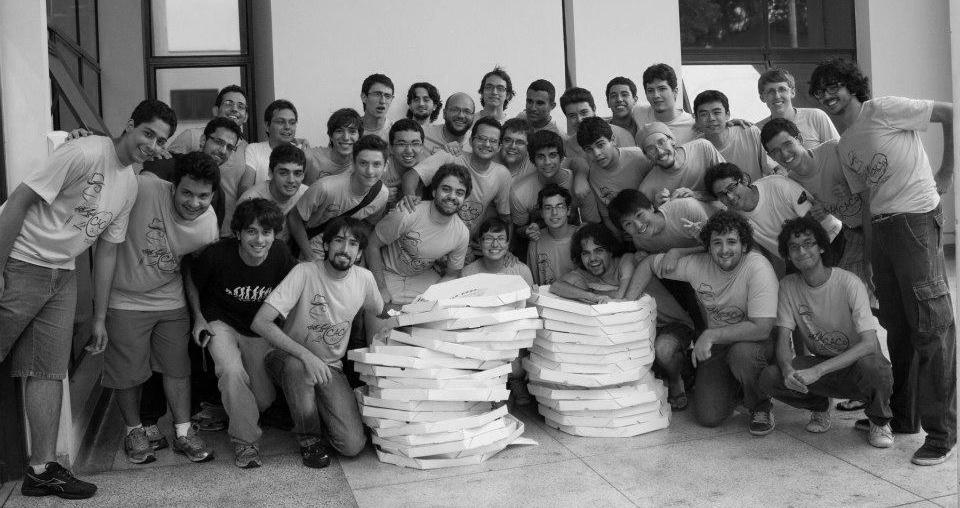
\includegraphics[scale=0.22]{img/caco/pizzada.jpg}
\end{figure}

O CACo tem como função representar os estudantes no âmbito acadêmico, ou seja,
perante o IC, a FEEC e a Unicamp. Mas o que o CACo faz? De forma
simplificada, procuramos ser porta-voz dos alunos. Reivindicamos espaço físico
decente para os alunos, alteração nas matérias e professores, promovemos
discussões sobre temas polêmicos e delicados, dentre muitas outras atividades.

Quer um exemplo? Esse estupendo manual que você está lendo neste exato momento
foi confeccionado pelo seu centro acadêmico para lhe ajudar no início da sua
vida universitária e, na verdade, você ainda vai se pegar recorrendo ao seu
Manual várias vezes durante seus quatro, cinco, doze anos na Unicamp.

Uma grande função do CACo é prezar pela qualidade dos cursos e fazemos isso, por
exemplo, através de discussões com o próprio Instituto, onde levamos reclamações
e reivindicações dos alunos para os coordenadores e professores.

\begin{figure}[H]
    \centering
    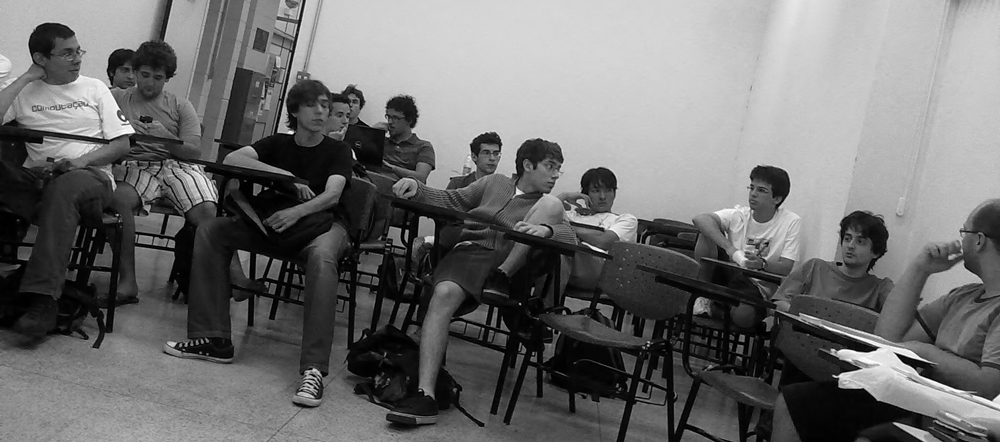
\includegraphics[scale=0.21]{img/caco/reuniao.jpg}
\end{figure}

Uma outra função do CACo é integrar os estudantes de computação da Unicamp. Para
isso, realizamos diversos eventos como o CineCACo, o PipoCACo, o CACo Games, o
CACo Series of Poker e a grande comemoração do Aniversário do CACo, que contou
com pizza de graça para mais de duzentos alunos! Tentamos também facilitar a
vida da galera através dos armários que alugamos, o Banco de Livros, o Banco de
Provas (o maior da Unicamp) e a máquina de café que colocamos no IC.

Repetindo o que foi dito antes: bixo, o CACo é o \textbf{seu} Centro Acadêmico.
Tudo que dissemos que fazemos pelos alunos, queremos fazer por você também. Por
isso, quando houver algum problema envolvendo a FEEC, o IC, os professores ou
qualquer coisa do tipo, não hesite em nos procurar. O CACo sempre lhe dará todo
o suporte necessário. Se tiver reclamação ou sugestão relacionada ao próprio
CACo, também estaremos aqui para ouvir. Mais do que isso, venha participar de
uma de nossas reuniões, que são abertas a você e todos os alunos de computação
da Unicamp.

\begin{figure}[H]
    \centering
    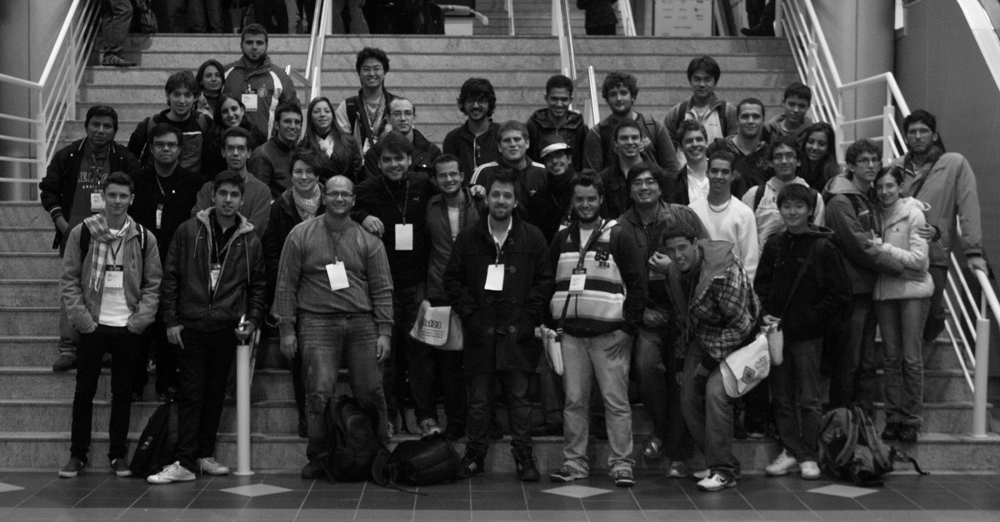
\includegraphics[scale=0.21]{img/caco/fisl2.jpg}
\end{figure}

Participar do CACo é uma experiência diferente de tudo aquilo que você terá na
sua graduação. É a chance de aprender e crescer de uma forma que não acontece em
nenhuma aula de cálculo. É uma oportunidade de conhecer seus veteranos e também
seus amiguinhos bixos. Mas, acima de tudo, é uma experiência pessoal onde você
vai aprender a se expressar, argumentar, defender suas ideias, falar em público
e pensar no coletivo. Você entrará em contato com muita gente que provavelmente
você nunca iria conhecer e, com certeza, fará amizade com muitos deles. Por
esses e muitos outros motivos é que você, bixo, deve vir a pelo menos uma
reunião do CACo e sentir na pele tudo o que foi dito aqui. Venha nos ajudar a
fortalecer ainda mais o melhor CA da Unicamp. Até a reunião!

\begin{compactitemize}
\item  E-mail: \email{caco@ic.unicamp.br}
\item  Site: \url{www.caco.ic.unicamp.br}
\item  Reuniões: você será informado no começo do semestre sobre os horários das reuniões. Participe!
\end{compactitemize}

Veja a seguir algumas das atividades que o CACo pratica:

\subsection{Avaliação de Curso e Reforma Curricular}

Uma vez por semestre, ocorre a reunião de avaliação de curso da qual participam
alunos, coordenadores e professores, além de responsáveis pela infraestrutura do
IC e da FEEC. Nela, são discutidos problemas relativos aos cursos, que vão desde
professores ruins até cadeiras quebradas. São avaliadas as disciplinas,
apontados problemas e indicadas soluções. A participação dos alunos é muito
importante, afinal somos nós que mais ganhamos e perdemos com o bom e o ruim de
nossos cursos. Por isso, o CACo participa dessa reunião levando a opinião dos
alunos para serem debatidas.

A avaliação de curso também visa a reforma curricular dos cursos. O catálogo do
curso (disciplinas que devem ser cursadas) é alterado todos os anos e a reunião
de avaliação tem grande papel nessas alterações.

\subsection{Caravana para o fisl}

O CACo organiza anualmente uma caravana para o fisl, o Fórum Internacional de
Software Livre, que acontece em Porto Alegre. O fisl reúne milhares de pessoas
de todo o mundo e conta com palestras e profissionais de renome. O Fórum é um
ótimo modo de entrar em contato com o mundo da computação e a caravana é uma
ótima e barata maneira de ir e tembém de socializar com outros computeiros.

\begin{figure}[H]
    \centering
    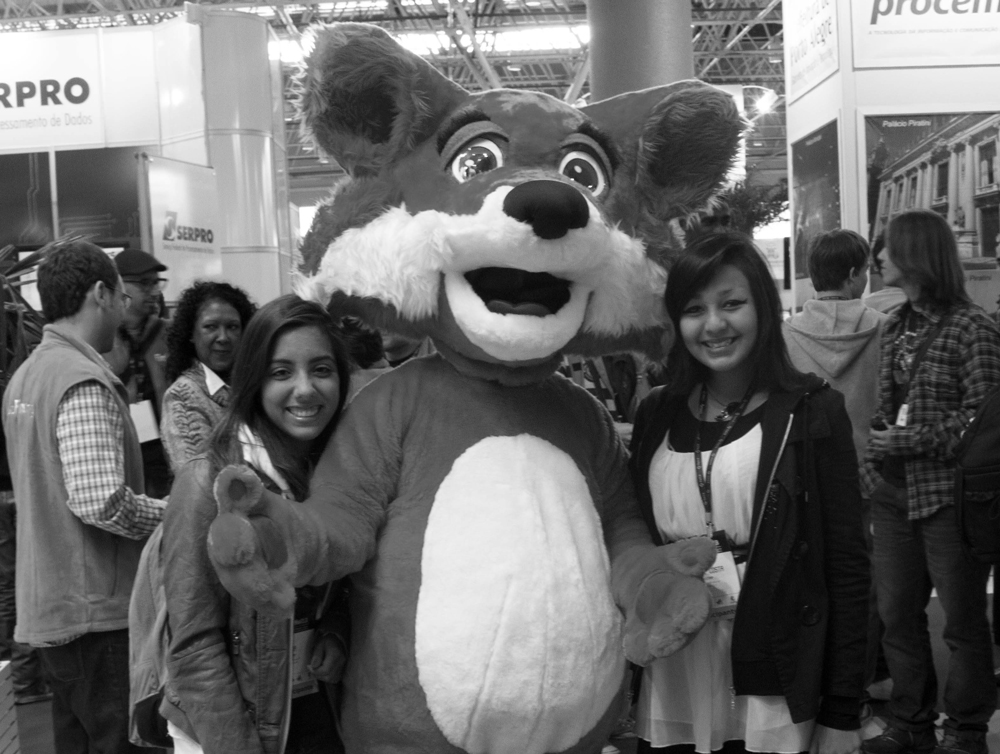
\includegraphics[scale=0.21]{img/caco/fisl.jpg}
\end{figure}

\subsection{Pesquisa Salarial}

Em 2010, com a colaboração do diretor do IC, o professor Hans Liesenberg,
e da rede social Reunion, promovemos uma pesquisa salarial com
ex-alunos de computação, que ajudou a fornecer um bom panorama da realidade em que se encontra
o profissional formado pela Unicamp na área de computação. A pesquisa
está disponível no site do CACo.

\subsection{CineCACo}

Por que não juntar com a galera no IC para assistir um filme com pipoca e
refriegerante de graça?

\subsection{PipoCACo}

Os PipoCACos são eventos de discussão sobre assuntos polêmicos, mas sem
comentários sobre  mamilos. Trata-se de um espaço para que toda a Computação
possa discutir um assunto de interesse geral. Por exemplo, já realizamos
PipoCACos sobre cotas em universidades públicas, sobre o Enade e semestralmente fazemos o PipoCACo de
Avaliação de Curso, onde reunimos as reclamações dos alunos para a reunião de
avaliação. Além de um ótimo local para ouvir opiniões e debater, os PipoCACos
são regados a refrigerante e pipoca por nossa conta!

\subsection{Palestra Azoide/Bzoide}

Chega um momento na vida de todo computeiro engenheiro em que ele deve responder
às questões fundamentais como: De onde viemos? Para onde vamos? Onde vamos
almoçar hoje? Vou ser Azoide ou Bzoide?

O curso de Engenharia de Computação da Unicamp se divide em duas habilitações, também conhecidas como modalidades: AA
e AB. A diferença? Não é simples! Por isso, o CACo organiza uma série de
palestras a fim de ajudá-lo a escolher a modalidade que mais lhe agrada.

\subsection{CACo Series of Poker}

O lendário torneio de Poker do CACo. Aberto a toda a computação, o CSoP é um
ótimo evento de integração e já contou com cinco edições de absoluto sucesso!
Você será informado da data do próximo, fique ligado!

\begin{figure}[H]
    \centering
    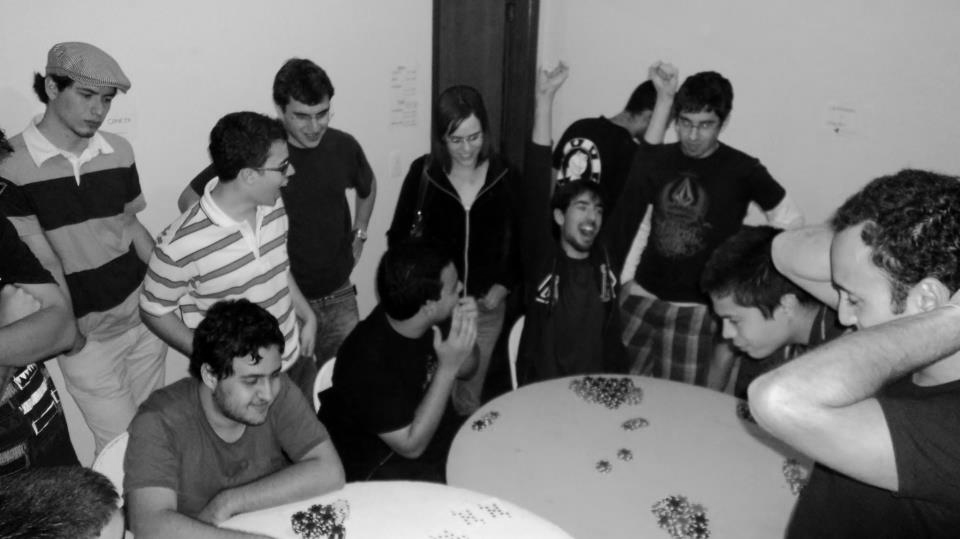
\includegraphics[scale=0.21]{img/caco/poker2.jpg}
\end{figure}

\subsection{Salinha}

A sede do CACo fica na nossa salinha no IC-3. Munida de uma incrível mesa de
sinuca, ela está aberta 24/7 para todos os computeiros que queiram jogar.

\subsection{Atendimento}

O CACo realiza atendimentos na nossa salinha. Nesses horários, você poderá
comprar nossos produtos, se inscrever em algum de nossos eventos ou só bater papo
com a gente mesmo. Os horários de atendimento serão divulgados no início do
semestre e você pode conferi-los no site do CACo.

\begin{figure}[H]
    \centering
    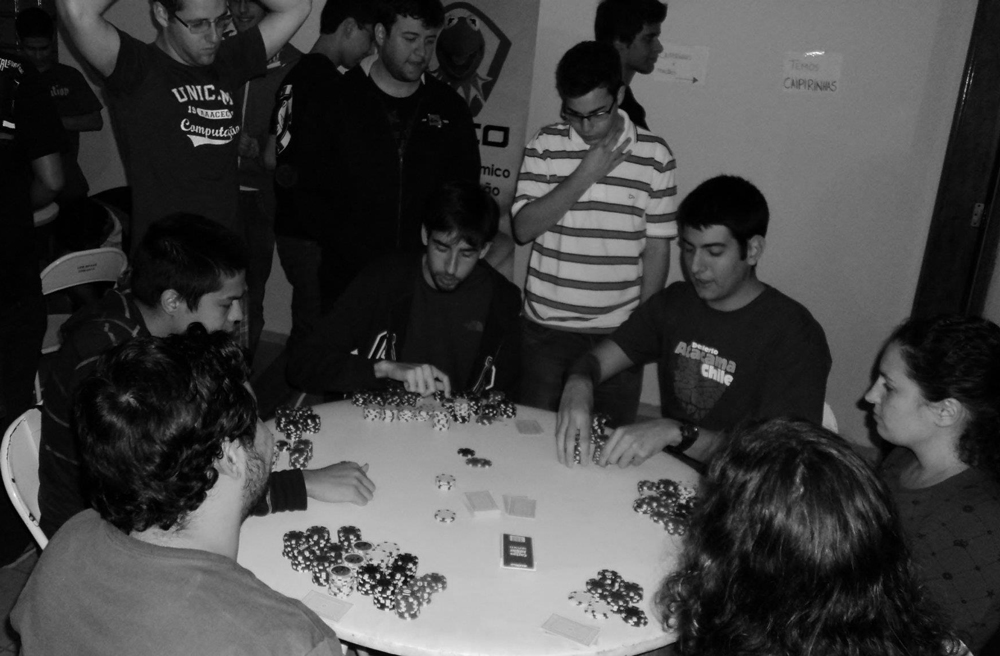
\includegraphics[scale=0.21]{img/caco/poker.jpg}
\end{figure}

\subsection{Gestão}

O CACo tem uma gestão composta de gente bonita e charmosa. Não se preocupe, se
você não é bonito nem charmoso, você ainda pode entrar na gestão... talvez. A
atual gestão foi eleita em novembro de 2012 e deve permanecer até outubro de
2013. Mas não pense que só a gestão gere o CACo. Mais uma vez: o CACo é o seu
centro acadêmico. Você e toda a computação também fazem parte do CACo e têm papel
nas nossas decisões e discussões.

Para ficar mais integrado ao que ocorre no seu centro acadêmico, como suas
ações, projetos e quais os problemas atuais, você pode se increver na lista do
CACo no Google Groups por meio do link:
\url{groups.google.com/group/cacounicamp}.

\begin{figure}[H]
    \centering
    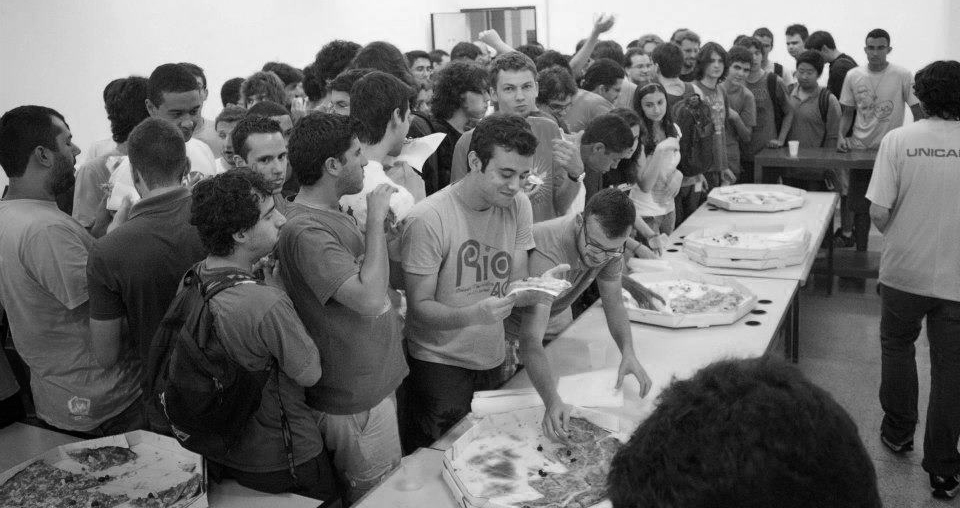
\includegraphics[scale=0.21]{img/caco/pizzada2.jpg}
\end{figure}

\begin{figure}[H]
    \centering
    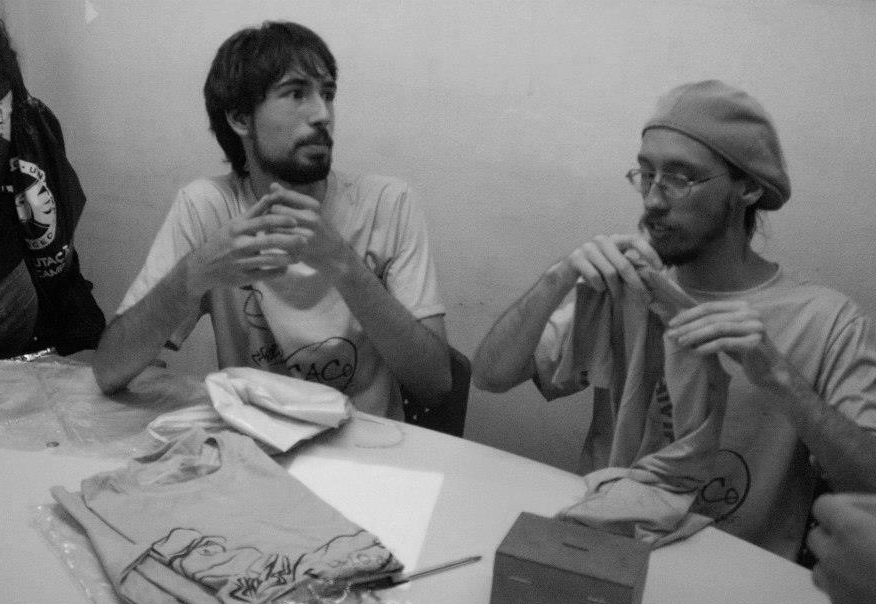
\includegraphics[scale=0.24]{img/caco/eleicao.jpg}
\end{figure}

\subsubsection{Chapa ``CACoCota'' (2012/2013)}

\begin{itemize}
\item   \textbf{Presidência}
		\\Julia Ramos Beltrão (Julia EC011)

\item   \textbf{Coordenadoria Administrativa}
		\\Alexandre Novais de Medeiros (Salsicha CC011)
		\\Victor Rodrigues Matsuguma (Preciso EC011)

\item   \textbf{Coodenadoria Financeira}
		\\Gabriel Militão Vinhas Lopes (Gagau EC012)
		\\André Felipe Barros Selva (Selva EC09)
		\\Guilherme Bueno Andrade (Laika EC012)

\item   \textbf{Coordenadoria de Ensino e Graduação}
		\\Pedro Henrique Azevedo Amorim (Amorim EC011)
		\\Brunno Rodrigues Arangues (Brunno EC010)

\item   \textbf{Coordenadoria de Ensino e Pós-Graduação}
		\\Eric Velten de Melo (Eric EC07)

\item   \textbf{Coordenadoria de Comunicação}
		\\Pedro Cordeiro de Almeida (Pedroka CC012)
		\\Yuri Corrêa Pinto Soares (Yuri CC012)
		\\Gérson de Paulo Carlos (Gérson EC09)

\item   \textbf{Coordenadoria de Eventos e Cultura}
		\\Antonio José Pinheiro Prado (Alegria EC012)
		\\Murilo Vieira Santa Bárbara (Buxexa EC012)
		\\Wesley Marques Dias (Kiabbo EC010)
		\\Humberto Aboud Torres Lobo (Sheldon EC010)
		\\Gustavo Menezes Rocha (Espanhol EC011)
		\\William Hideki Azana Tustumi (William EC011)

\item   \textbf{Coordenadoria de Marketing}
		\\Matheus Jun Ota (Ota CC012)
		\\Gabriel Rolfsen Franzoni (Clits EC012)
		\\Thiago Rosario Caetano (Thiago EC010)
		\\Jucélio Evangelista Fonseca (Jeff CC012)

\item   \textbf{Coordenadoria de Produtos}
		\\Hugo Aboud Torres Lobo (Hugo EC012)
		\\José Américo Nabuco Leva Ferreira de Freitas (Jota EC010)

\item   \textbf{Coordenadoria Tecnológica}
		\\Gabriel Hidasy Rezende (Sam EC011)
		\\Gustavo de Mello Crivelli (Jobs EC012)
		\\Matheus Mostiack Pomaleski (Poma EC011)
		\\Pedro Emílio Machado de Brito (Asmina EC012)

\end{itemize}

As gestões dos anos anteriores podem ser vistas no site do CACo.

\begin{figure}[H]
    \centering
    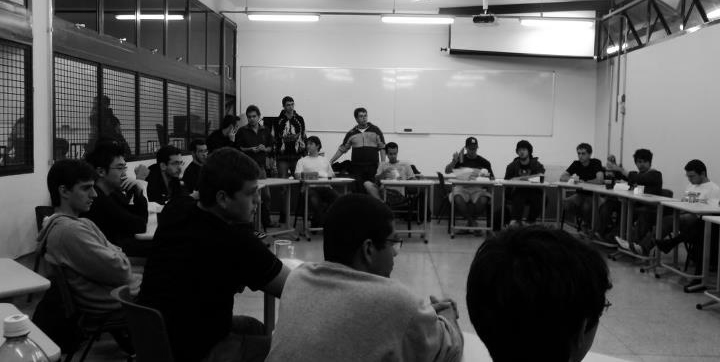
\includegraphics[scale=0.29]{img/caco/pipocaco.jpg}
\end{figure}


%%%%% Jornal da Unicamp
%%%%% Eventos da Unicamp
%%%%% Pra que que eu estou estudando isso??
% Este arquivo tex vai ser incluído no arquivo tex principal, não pe preciso
% declarar nenhum cabeçalho

\section{Jornal da Unicamp}

O jornal da Unicamp é um jornal de distribuição semanal distribuído dentro da
Unicamp. Podem-se encontrar diversos exemplares do jornal na sala de computadores
que fica ao lado da DAC, no IC-2 e em diversos pontos espalhado pelo campus.

No jornal são mostradas as diversas pesquisas realizadas pela universidade,
eventos, livros e obras de autoria de professores, aparições da Unicamp na
imprensa e defesas de mestrado e doutorado.

Na página do jornal (\url{http://www.unicamp.br/ju}) pode-se encontrar as
últimas edições do jornal (em PDF), além de poder fazer a assinatura online do
jornal, distribuído em formato PDF. A assinatura e distribuição do jornal são
gratuitas.

\section{Eventos da Unicamp}
\subsection{Feira do Livro}

Evento iniciado em 2002, a cada dois anos a Editora da Unicamp realiza a Feira
do Livro, no Ginásio da Unicamp. Há excelentes opções, de diversas editoras,
principalmente na área de literatura, artes e humanas, com no mínimo 50\% de
desconto.

\subsection{Semanas da Unicamp}

Alguns cursos da Unicamp realizam anualmente um evento (chamado de semana) em
que os alunos de graduação têm um contato com o mercado de trabalho, com as
pesquisas, com as tendências e novidades dos cursos e demais assuntos, ramos
e áreas de cada curso. Para isso, participam desse evento ex-alunos
e profissionais, realizam-se palestras e minicursos, são feitas visitas
a empresas e são feitos debates ("mesas redondas").

A computação tem a sua semana. É o Computação e Mercado (C\&M), que é realizado
pela conpec desde 1993.

\subsection{Talento}

Talento é um evento que acontece todo ano, desde 1999, durante um dia inteiro,
no Ginásio Multidisciplinar e organizado pelo Núcleo de Empresas Juniores da
Unicamp. Trata-se de uma feira de recrutamento, onde alunos da Unicamp e de
outras universidades e o público em geral têm contato com empresas, seja por
meio de palestras, mesas redondas e estandes, e estas apresentam o seu processo
seletivo. Nesse evento também é feito o cadastro de currículos dos visitantes.

Para saber mais sobre o evento, é só acessar a página da Talento
(\url{http://www.talentounicamp.com.br/}). O evento é gratuito.

\subsection{UPA -- Unicamp de Portas Abertas}

Desde 2003 acontece a UPA (Unicamp de Portas Abertas). Esse evento é um
aprimoramento de um evento que acontecia há alguns anos atrás, a Universidade
Aberta ao Público.

A UPA é um evento anual, em que, durantes dois dias (geralmente dois dias do mês
de setembro) a Unicamp é apresentada para estudantes dos ensinos fundamental
e médio de todo o país (muitos desses alunos sendo pré-vestibulandos). A apresentação
da universidade é feita por professores e alunos, que mostram as salas de aula
e as pesquisas realizadas.

No ano de 2007, a UPA recebeu a visita de 50 mil alunos de 950 escolas públicas
e privadas de 10 estados.

Para saber mais sobre o evento, é só acessar a página
\url{http://www.upa.unicamp.br/}.

\section{Pra que que eu estou estudando isso??}

O ensino médio acabou, você finalmente está livre de todas as inutilidades, como
química orgânica e separação silábica de verbos parnasianos, só vai ver coisas
relevantes para a profissão, e{\dots}

Pimba! HZ291. Pode, Arnaldo?

Primeiro, você precisa saber que a Universidade não é um curso técnico. A ideia
não é só te dar capacitação profissional, mas sim formar pessoas melhores. Para
que um computeiro precisa de contabilidade? Para nada, mas uma pessoa (de exatas
pelo menos) precisa ter uma noção disso.

Outro problema: o que exatamente é "relevante para a sua profissão"?
A computação é uma área muito vasta, e a graduação (o curso que você tá
fazendo{\dots}) é bem generalista, para te dar base para escolher. Por exemplo,
vai ter gente que nunca mais vai usar GA/Algelin, mas quem for para a área de
computação gráfica vai comer matriz no café da manhã. Quem garante que no meio
do curso você não decida ir para essa área? Ou ainda, que no seu emprego não te
joguem um problema desse tipo?

Se você continuar na Universidade, na pós você só terá matérias da sua área, já
que você já sabe o suficiente pra dizer que área é essa. Mas ainda falta muito
chão até lá{\dots}

Pra quem é da engenharia, um problema maior é que, para conseguir o CREA,
existem algumas matérias obrigatórias (embora completamente inúteis, sem
exagero), como ResMat. A Unicamp até pode contrariar essas orientações, até
certo ponto, mas dificilmente os professores concordariam. (Por outro lado,
você poderá construir prédios de até 2 andares. Recomendamos fortemente que você
não faça isso.)

Para quem é da ciência, o curso não é para formar "programadores". Vocês serão
mais que isso, serão cientistas, e isso envolve ver coisas além de só código.

Nesse manual não temos muito espaço pra falar em detalhes. Para dar uma noção
mais específica da utilidade (ou não) de cada matéria, fizemos uma wiki, que você
pode acessar aqui:
\url{http://www.caco.ic.unicamp.br/wiki/index.php/Wiki_de_Matérias}


%%%% Contra capa
\pagebreak{4}

\thispagestyle{empty}
\ThisTileWallPaper{\paperwidth}{\paperheight}{img/contracapa.png}

%%%% Final da contra capa

\end{document}
